%input macros (i.e. write your own macros file called MacroFile1.tex)
%\newcommand{\PdfPsText}[2]{
  \ifpdf
     #1
  \else
     #2
  \fi
}

\newcommand{\IncludeGraphicsH}[3]{
  \PdfPsText{\includegraphics[height=#2]{#1}}{\includegraphics[bb = #3, height=#2]{#1}}
}

\newcommand{\IncludeGraphicsW}[3]{
  \PdfPsText{\includegraphics[width=#2]{#1}}{\includegraphics[bb = #3, width=#2]{#1}}
}

\newcommand{\InsertFig}[3]{
  \begin{figure}[!htbp]
    \begin{center}
      \leavevmode
      #1
      \caption{#2}
      \label{#3}
    \end{center}
  \end{figure}
}


%%% Local Variables: 
%%% mode: latex
%%% TeX-master: "~/Documents/LaTeX/CUEDThesisPSnPDF/thesis"
%%% End: 


 \documentclass[oneside,11pt]{Classes/CUEDthesisPSnPDF}


\ifpdf
    \pdfinfo { /Title  (CUED PhD and MPhil Thesis Classes)
               /Creator (TeX)
               /Producer (pdfTeX)
               /Author (Mian Asbat Ahmad mian.ahmad@york.ac.uk)
               /CreationDate (D:20030101000000)  %format D:YYYYMMDDhhmmss
               /ModDate (D:20030815213532)
               /Subject (Writing a PhD thesis in LaTeX)
               /Keywords (PhD, Thesis)}
    \pdfcatalog { /PageMode (/UseOutlines)
                  /OpenAction (fitbh)  }
\fi

\title{New Strategies for Automated Random Testing\\[1ex]}

\ifpdf
  \author{\href{mailto:mian.ahmad@york.ac.uk}{Mian Asbat Ahmad}}
  \collegeordept{\href{http://www.cs.york.ac.uk}{Department of Computer Science}}
  \university{\href{http://www.york.ac.uk}{The University of York}}
% insert below the file name that contains the crest in-place of 'UnivShield'
  %\crest{
\includegraphics[width=30mm]{UnivShield}}
\else
  \author{Mian Asbat Ahmad}
  \collegeordept{Department of Computer Science}
  \university{The University of York}
% insert below the file name that contains the crest in-place of 'UnivShield'
  %\crest{
\includegraphics[bb = 0 0 292 336, width=30mm]{UnivShield}}
\fi
%
% insert below the file name that contains the crest in-place of 'UnivShield'
% \crest{\IncludeGraphicsW{UnivShield}{40mm}{14 14 73 81}}
%
%\renewcommand{\submittedtext}{change the default text here if needed}
\degree{Doctor of Philosophy}
\degreedate{\today}

% turn of those nasty overfull and underfull hboxes
\hbadness=10000
\hfuzz=50pt

% Put all the style files you want in the directory StyleFiles and usepackage like this:
\usepackage{multirow}
\usepackage{StyleFiles/watermark}
\usepackage{amssymb}
\usepackage{graphicx}
%\usepackage{epstopdf}
\usepackage{amsmath,epsfig}
\usepackage{times}
\usepackage{float}
\usepackage{epsfig}
\usepackage{latexsym}
\usepackage{enumerate}
\usepackage{url}
\usepackage{subfigure}
\usepackage{rotating}
\usepackage{verbatim}
\usepackage{tabularx}
\usepackage{amsmath}
\usepackage{listings}
\usepackage{color}
\definecolor{javared}{rgb}{0.6,0,0} % for strings
\definecolor{javagreen}{rgb}{0.25,0.5,0.35} % comments
\definecolor{javapurple}{rgb}{0.5,0,0.35} % keywords
\definecolor{javadocblue}{rgb}{0.25,0.35,0.75} % javadoc

\lstset{language=Java,
basicstyle=\ttfamily,
keywordstyle=\color{javapurple}\bfseries,
stringstyle=\color{javared},
commentstyle=\color{javagreen},
morecomment=[s][\color{javadocblue}]{/**}{*/},
%numbers=left,
numberstyle=\tiny\color{black},
stepnumber=2,
numbersep=10pt,
tabsize=4,
showspaces=false,
showstringspaces=false}

% Comment out the next line to get single spacing
\onehalfspacing

\begin{document}

%\language{english}

% A page with the abstract on including title and author etc may be
% required to be handed in separately. If this is not so, then comment
% the below 3 lines (between '\begin{abstractseparte}' and
% 'end{abstractseparate}'), normally like a declaration ... needs some more
% work, mind as environment abstracts creates a new page!
% \begin{abstractseparate}
%   \begin{abstract}

%Software testing is the process of evaluating the quality of a software or its component.The thesis presents new techniques for improving the effectiveness of automated random testing, evaluates the efficiency of these techniques and proposes directions for future work.
%, is a well used approach for detecting software failures. Testing involves generation and execution of test inputs and evaluation of results for correctness either manually or by automatic means. Automated software testing save time and human effort involved in manual testing. There are two major challenges in software testing: the generation of appropriate test inputs and evaluation of the test results. This thesis addresses both issues.

%Exhaustive testing is not feasible in most cases and a test strategy is often used to select a small subset of the inputs for testing of software. Selection of adequate test strategy is crucial for better test performance because the chances of finding failures increases if the selected subset of data effectively represents the whole input domain. 


The ever increasing reliance on software-intensive systems is driving research to discover software faults more effectively and more efficiently. Despite intensive research, very few approaches have studied and used knowledge about fault domains to improve the testing or the feedback given to developers. The present thesis addresses this shortcoming: it leverages fault co-localization in a new random testing strategy called Dirt Spot Sweeping Random (DSSR), and it presents two new strategies: Automated Discovery of Failure Domain (ADFD) and Automated Discovery of Failure Domain$^+$ (ADFD$^+$). These improve the feedback given to developers by deducing more information about the failure domain (i.e. point, block, strip) in an automated way.
%Testing a software with all permutations and combinations of inputs is not feasible because of infinite possible scenarios. Alternatively, a strategy is used to select a small subset of inputs for testing software. Random strategy is a viable option to generate comparatively cheap test inputs without too much intellectual and computational efforts. However, arbitrarily generating test inputs without any help from available information may be effective in some cases but generally results in vague or unnecessary test inputs.  
%The strategy which uses a truly representative subset of the input domain increases the chances of detecting higher number of failure in the software.  
%The thesis addresses the issues and presents three new automated random testing strategies developed by manipulating the patterns of failure domains within the input domain. 
%The strategies have been experimentally evaluated for effectiveness and efficiency. The characteristics of failure domains and their influence on the performance of the test strategies have been examined. 
The DSSR strategy adds the value causing the failure and its neighbouring values to the list of interesting values for exploring the underlying failure domain. The comparative evaluation showed significantly better performance of DSSR over Random and Random$^+$ strategies. The ADFD strategy finds failures and failure domains and presents the pass and fail domains in graphical form. The results obtained by evaluating error-seeded numerical programs indicated highly effective performance of the ADFD strategy. The ADFD$^+$ strategy is an extended version of ADFD strategy with respect to algorithm and graphical presentation of failure domains. In comparison with Randoop, ADFD$^+$ strategy successfully detected all failures and failure domains while Randoop identified individual failures but could not detect failure domains. 
%To determine the precision of identifying failure domains by ADFD and ADFD+, Daikon was integrated in the two techniques and extensive experimental analyses of real world Java projects contained in Qualitas Corpus were performed. The results obtained were analysed and cross-checked by manual testing. 
The ADFD and ADFD$^+$ techniques were enhanced by integration of the automatic invariant detector Daikon, and the precision of identifying failure domains was determined through extensive experimental evaluation of real world Java projects contained in a database, namely Qualitas Corpus. The analyses of results, cross-checked by manual testing indicated that ADFD and ADFD$^+$ techniques are highly effective in providing assistance but are not an alternative to manual testing.

%These results provide a thorough understanding of automated random testing and leads to several researchable areas indicated in the thesis.


%The chapter evaluates the precision of identifying failure domains by the enhanced ADFD and ADFD+ techniques integrated with the automatic tool Daikon. Extensive experimental analysis of real world Java projects contained in Qualitas Corpus were performed. The results obtained were analysed and cross-checked with the results of manual testing. The results reveal that the two techniques can effectively identify and present all types of failure domains (graphically by JFreeChart and as invariants by Daikon) to a certain level of precision. It is also evident that the level of precision of identifying failure domain can be further increased graphically and invariantly by increasing the range value in the two techniques. The analysis revealed that the strip failure domain having large size and low complexity are quickly identified by the automated techniques whereas the point and block failure domains having small size and higher complexity are difficultly identified by the auto- mated and manual techniques. Based on the results, it can also be stated that automated techniques (ADFD and ADFD+) can be highly effective in providing assistance to manual testing but are not an alternative to the manual testing. 











%To find the comparative effectiveness of ADFD and ADFD+ strategies, both techniques were integrated with automated invariant detector Daikon. Extensive experimental analysis of Java projects contained in Qualitas Corpus was carried out in comparison with manual technique. The results revealed 



%Evaluation of the precision of identifying failure domains by ADFD and ADFD+. For the purpose of comparative analysis, Daikon has been integrated in the two techniques and extensive experimental analyses of real world Java projects contained in Qualitas Corpus are performed. The results obtained are analysed and cross-checked with the results of Manual testing. The impact of nature, location, size, type and complexity of failure domains on the testing techniques are reflected.



%This thesis presents new automated random testing strategies developed by manipulating the patterns of failure domains within the input domain. The strategies have been experimentally evaluated for effectiveness and efficiency. The characteristics of failure domains and their influence on the performance of the test strategies has been examined. A brief introduction is given in Chapter~\ref{Introduction1} which is followed by a detailed review of the relevant literature in Chapter~\ref{chap:softwareTesting}. Chapter~\ref{chap:yeti_3} includes a thorough review of YETI, that has been used as a platform to host the strategies and conduct the experiments. Chapter~\ref{chap:DSSR} describes the DSSR strategy based on the dirt spot sweeping phenomenon that adds the value causing the failure and its neighbouring values to the list if interesting values for exploring the underlying failure domain. The comparative evaluation showed significantly better performance of DSSR over R and R$^+$ strategies. Chapter~\ref{chap:ADFD} presents the Automated Discovery of Failure Domain (ADFD) strategy developed with the ability to find failure, failure domains and provides visualisation of pass and fail domain. The experimental results by applying ADFD strategy to error-seeded programs indicate that the strategy is highly effective in identifying the failure domains. Chapter~\ref{chap:ADFD+} presents the Automated Discovery of Failure Domain$^+$ (ADFD$^+$) strategy. It is an upgraded version of ADFD strategy with respect to the algorithm and graphical representation of failure domains. The ADFD$^+$ strategy compared with Randoop under identical conditions successfully detected all failure domains as against Randoop, which identified individual failures but was unable to detect the failure domains. {Chapter~\ref{chap:Evaluation}} presents extensive experimental analysis of Java projects contained in Qualitas Corpus to find the effectiveness of the two automated techniques (ADFD and ADFD$^+$) in comparison with manual technique. The results revealed significance of the two techniques and also provide an insight into the types, frequencies, nature of failure domains and their effect on the testing techniques in production software. {Chapter~\ref{chap:conclusions_8}} includes conclusions, contributions and the lessons learned. Finally, {Chapter~\ref{chap:futureWork}} highlights the opportunities for future work, challenges and likely solutions.

%The types, frequencies, nature of failure domains and their effect on the testing techniques in production software were explored. {Chapter~\ref{chap:conclusions_8}} includes conclusions, contributions and the lessons learned. Finally, {Chapter~\ref{chap:futureWork}} highlights the opportunities for future work, challenges and likely solutions.


%Software is an important and essential component of computer system without which no task can be accomplished. Software testing, the process of evaluating the correctness and quality of a software or its component, is the most widely adapted method for detecting software failures. For program testing, test inputs are generated, executed and the results are evaluated for correctness. Automated software testing is performed to save time and human effort involved in manual testing. The two major challenges in automated testing i.e. the generation of appropriate test inputs and evaluation of the test results need to be addressed.

%The present work is an addition to the literature aiming at reducing the overall cost of software testing by devising new, improved and  effective automated software testing techniques based on random strategy. The first new technique named as Dirt Spot Sweeping Random (DSSR) strategy was developed on the assumption that unique failures reside in contiguous block strips. When a failure is identified, the DSSR strategy selects the neighbouring input values except duplicate values for the subsequent tests. The selected values sweep around the identified failure, leading to the discovery of new failures in the vicinity. This results in quick and efficient identification of faults in Software Under Test (SUT). The second technique named as, Automated Discovery of Failure Domain (ADFD) was developed with the capability to find faults as well as the fault domains in a given SUT and provides visualization of the identified pass and fail domains within a specified range in the form of a chart. The new technique is highly effective in testing and debugging and provides an easy to understand test report in the visualized form. The third new technique proposed in the research study is, Invariant Guided Random$^+$ Strategy (IGRS) which is an extended form of Random$^+$ strategy guided by software invariants. In this technique, Invariants from the given SUT are automatically collected by Daikon tool, filtered through DynComp and annotated in the source code as assertions. (The experiments are in progress, the results obtained will be compared with the DSSR, Random and Random$^+$ strategies and the findings will be included in the thesis and abbreviated in the abstract as soon as possible.)

\end{abstract}
% \end{abstractseparate}


%%%%%%%%%%%%%%%%%%%%%%%%%%%%%%%%%%%%%%%%%%%%%%%%%%%%%%%%%%%%%%%%%%%%%
%%%%%%%%%%%%%%%%%%%%%%%%%%%%%%%%%%%%%%%%%%%%%%%%%%%%%%%%%%%%%%%%%%%%%
%%%%%%%%%%%%%%%%%%%%%%%%%%%%%%%%%%%%%%%%%%%%%%%%%%%%%%%%%%%%%%%%%%%%%
%%%%%%%%%%%%%%%%%%%%%%%%%%%%%%%%%%%%%%%%%%%%%%%%%%%%%%%%%%%%%%%%%%%%%
%%%%%%%%%%%%%%%%%%%%%%%%%%%%%%%%%%%%%%%%%%%%%%%%%%%%%%%%%%%%%%%%%%%%%
% Using the watermark package which is in StyleFiles/
% and to remove DRAFT COPY ONLY appearing on the top of all pages comment out below line
%\watermark{DRAFT COPY ONLY}


\maketitle

%set the number of sectioning levels that get number and appear in the contents
\setcounter{secnumdepth}{3}
\setcounter{tocdepth}{3}

\frontmatter % book mode only
\pagenumbering{roman}

\begin{abstract}

%Software testing is the process of evaluating the quality of a software or its component.The thesis presents new techniques for improving the effectiveness of automated random testing, evaluates the efficiency of these techniques and proposes directions for future work.
%, is a well used approach for detecting software failures. Testing involves generation and execution of test inputs and evaluation of results for correctness either manually or by automatic means. Automated software testing save time and human effort involved in manual testing. There are two major challenges in software testing: the generation of appropriate test inputs and evaluation of the test results. This thesis addresses both issues.

%Exhaustive testing is not feasible in most cases and a test strategy is often used to select a small subset of the inputs for testing of software. Selection of adequate test strategy is crucial for better test performance because the chances of finding failures increases if the selected subset of data effectively represents the whole input domain. 


The ever increasing reliance on software-intensive systems is driving research to discover software faults more effectively and more efficiently. Despite intensive research, very few approaches have studied and used knowledge about fault domains to improve the testing or the feedback given to developers. The present thesis addresses this shortcoming: it leverages fault co-localization in a new random testing strategy called Dirt Spot Sweeping Random (DSSR), and it presents two new strategies: Automated Discovery of Failure Domain (ADFD) and Automated Discovery of Failure Domain$^+$ (ADFD$^+$). These improve the feedback given to developers by deducing more information about the failure domain (i.e. point, block, strip) in an automated way.
%Testing a software with all permutations and combinations of inputs is not feasible because of infinite possible scenarios. Alternatively, a strategy is used to select a small subset of inputs for testing software. Random strategy is a viable option to generate comparatively cheap test inputs without too much intellectual and computational efforts. However, arbitrarily generating test inputs without any help from available information may be effective in some cases but generally results in vague or unnecessary test inputs.  
%The strategy which uses a truly representative subset of the input domain increases the chances of detecting higher number of failure in the software.  
%The thesis addresses the issues and presents three new automated random testing strategies developed by manipulating the patterns of failure domains within the input domain. 
%The strategies have been experimentally evaluated for effectiveness and efficiency. The characteristics of failure domains and their influence on the performance of the test strategies have been examined. 
The DSSR strategy adds the value causing the failure and its neighbouring values to the list of interesting values for exploring the underlying failure domain. The comparative evaluation showed significantly better performance of DSSR over Random and Random$^+$ strategies. The ADFD strategy finds failures and failure domains and presents the pass and fail domains in graphical form. The results obtained by evaluating error-seeded numerical programs indicated highly effective performance of the ADFD strategy. The ADFD$^+$ strategy is an extended version of ADFD strategy with respect to algorithm and graphical presentation of failure domains. In comparison with Randoop, ADFD$^+$ strategy successfully detected all failures and failure domains while Randoop identified individual failures but could not detect failure domains. 
%To determine the precision of identifying failure domains by ADFD and ADFD+, Daikon was integrated in the two techniques and extensive experimental analyses of real world Java projects contained in Qualitas Corpus were performed. The results obtained were analysed and cross-checked by manual testing. 
The ADFD and ADFD$^+$ techniques were enhanced by integration of the automatic invariant detector Daikon, and the precision of identifying failure domains was determined through extensive experimental evaluation of real world Java projects contained in a database, namely Qualitas Corpus. The analyses of results, cross-checked by manual testing indicated that ADFD and ADFD$^+$ techniques are highly effective in providing assistance but are not an alternative to manual testing.

%These results provide a thorough understanding of automated random testing and leads to several researchable areas indicated in the thesis.


%The chapter evaluates the precision of identifying failure domains by the enhanced ADFD and ADFD+ techniques integrated with the automatic tool Daikon. Extensive experimental analysis of real world Java projects contained in Qualitas Corpus were performed. The results obtained were analysed and cross-checked with the results of manual testing. The results reveal that the two techniques can effectively identify and present all types of failure domains (graphically by JFreeChart and as invariants by Daikon) to a certain level of precision. It is also evident that the level of precision of identifying failure domain can be further increased graphically and invariantly by increasing the range value in the two techniques. The analysis revealed that the strip failure domain having large size and low complexity are quickly identified by the automated techniques whereas the point and block failure domains having small size and higher complexity are difficultly identified by the auto- mated and manual techniques. Based on the results, it can also be stated that automated techniques (ADFD and ADFD+) can be highly effective in providing assistance to manual testing but are not an alternative to the manual testing. 











%To find the comparative effectiveness of ADFD and ADFD+ strategies, both techniques were integrated with automated invariant detector Daikon. Extensive experimental analysis of Java projects contained in Qualitas Corpus was carried out in comparison with manual technique. The results revealed 



%Evaluation of the precision of identifying failure domains by ADFD and ADFD+. For the purpose of comparative analysis, Daikon has been integrated in the two techniques and extensive experimental analyses of real world Java projects contained in Qualitas Corpus are performed. The results obtained are analysed and cross-checked with the results of Manual testing. The impact of nature, location, size, type and complexity of failure domains on the testing techniques are reflected.



%This thesis presents new automated random testing strategies developed by manipulating the patterns of failure domains within the input domain. The strategies have been experimentally evaluated for effectiveness and efficiency. The characteristics of failure domains and their influence on the performance of the test strategies has been examined. A brief introduction is given in Chapter~\ref{Introduction1} which is followed by a detailed review of the relevant literature in Chapter~\ref{chap:softwareTesting}. Chapter~\ref{chap:yeti_3} includes a thorough review of YETI, that has been used as a platform to host the strategies and conduct the experiments. Chapter~\ref{chap:DSSR} describes the DSSR strategy based on the dirt spot sweeping phenomenon that adds the value causing the failure and its neighbouring values to the list if interesting values for exploring the underlying failure domain. The comparative evaluation showed significantly better performance of DSSR over R and R$^+$ strategies. Chapter~\ref{chap:ADFD} presents the Automated Discovery of Failure Domain (ADFD) strategy developed with the ability to find failure, failure domains and provides visualisation of pass and fail domain. The experimental results by applying ADFD strategy to error-seeded programs indicate that the strategy is highly effective in identifying the failure domains. Chapter~\ref{chap:ADFD+} presents the Automated Discovery of Failure Domain$^+$ (ADFD$^+$) strategy. It is an upgraded version of ADFD strategy with respect to the algorithm and graphical representation of failure domains. The ADFD$^+$ strategy compared with Randoop under identical conditions successfully detected all failure domains as against Randoop, which identified individual failures but was unable to detect the failure domains. {Chapter~\ref{chap:Evaluation}} presents extensive experimental analysis of Java projects contained in Qualitas Corpus to find the effectiveness of the two automated techniques (ADFD and ADFD$^+$) in comparison with manual technique. The results revealed significance of the two techniques and also provide an insight into the types, frequencies, nature of failure domains and their effect on the testing techniques in production software. {Chapter~\ref{chap:conclusions_8}} includes conclusions, contributions and the lessons learned. Finally, {Chapter~\ref{chap:futureWork}} highlights the opportunities for future work, challenges and likely solutions.

%The types, frequencies, nature of failure domains and their effect on the testing techniques in production software were explored. {Chapter~\ref{chap:conclusions_8}} includes conclusions, contributions and the lessons learned. Finally, {Chapter~\ref{chap:futureWork}} highlights the opportunities for future work, challenges and likely solutions.


%Software is an important and essential component of computer system without which no task can be accomplished. Software testing, the process of evaluating the correctness and quality of a software or its component, is the most widely adapted method for detecting software failures. For program testing, test inputs are generated, executed and the results are evaluated for correctness. Automated software testing is performed to save time and human effort involved in manual testing. The two major challenges in automated testing i.e. the generation of appropriate test inputs and evaluation of the test results need to be addressed.

%The present work is an addition to the literature aiming at reducing the overall cost of software testing by devising new, improved and  effective automated software testing techniques based on random strategy. The first new technique named as Dirt Spot Sweeping Random (DSSR) strategy was developed on the assumption that unique failures reside in contiguous block strips. When a failure is identified, the DSSR strategy selects the neighbouring input values except duplicate values for the subsequent tests. The selected values sweep around the identified failure, leading to the discovery of new failures in the vicinity. This results in quick and efficient identification of faults in Software Under Test (SUT). The second technique named as, Automated Discovery of Failure Domain (ADFD) was developed with the capability to find faults as well as the fault domains in a given SUT and provides visualization of the identified pass and fail domains within a specified range in the form of a chart. The new technique is highly effective in testing and debugging and provides an easy to understand test report in the visualized form. The third new technique proposed in the research study is, Invariant Guided Random$^+$ Strategy (IGRS) which is an extended form of Random$^+$ strategy guided by software invariants. In this technique, Invariants from the given SUT are automatically collected by Daikon tool, filtered through DynComp and annotated in the source code as assertions. (The experiments are in progress, the results obtained will be compared with the DSSR, Random and Random$^+$ strategies and the findings will be included in the thesis and abbreviated in the abstract as soon as possible.)

\end{abstract}

\tableofcontents
\listoffigures
\listoftables
\printnomenclature  %% Print the nomenclature
\addcontentsline{toc}{chapter}{Nomenclature}.

% Thesis Acknowledgements ------------------------------------------------


%\begin{acknowledgementslong} %uncommenting this line, gives a different acknowledgements heading
\begin{acknowledgements}      %this creates the heading for the acknowledgements


Several people have contributed to the completion of my PhD dissertation. However, the most prominent personality deserving due recognition is my worthy supervisor, Dr. Manuel Oriol. Thank you Manuel for your endless help, valuable guidance, constant encouragement, precious advice, sincere and affectionate attitude.

I thank my assessor Prof. John Clark for his constructive feedback on my various reports and presentations. I am also thankful and highly indebted to Prof. Richard Paige for his generous help, cooperation and guidance during my research at the University of York.

Special thanks to my father Prof. Mushtaq A. Mian who provided a conducive environment, valuable guidance and crucial support at all levels of my educational career and my very beloved mother whose love, affection and prayers have been my most precious assets. Also I am thankful to my elder brothers Dr. Ashfaq, Dr. Aftab, Dr. Ishaq, Dr. Afaq and my sister Dr. Haleema who have been the source of inspiration for me to pursue higher studies. My immediate younger brother Dr. Ilyas and my younger sister Ayesha studying in the UK, deserve recognition for their help, well wishes and moral support. Last but not the least I am very thankful to my dear wife Dr. Munazza for her company, help and cooperation throughout my stay at York.

I was funded by Departmental Overseas Research Scholarship (DORS), a financial support awarded to overseas students on the basis of outstanding academic ability and research potential. I am truly grateful to the Department of Computer Science for financial support that allowed me to concentrate on my research.


\end{acknowledgements}
%\end{acknowledgmentslong}

% ------------------------------------------------------------------------

%%% Local Variables: 
%%% mode: latex
%%% TeX-master: "../thesis"
%%% End: 

\include{Declaration/decleration}
\begin{dedication}
I feel it a great honour to dedicate my PhD thesis to my beloved parents and wife
for their significant contribution in achieving the goal of academic excellence.
\end{dedication}





\mainmatter % book mode only
%%% Thesis Introduction --------------------------------------------------
\chapter{Introduction}
%\ifpdf
%    \graphicspath{{Introduction/IntroductionFigs/PNG/}{Introduction/IntroductionFigs/PDF/}{Introduction/IntroductionFigs/}}
%\else
%    \graphicspath{{Introduction/IntroductionFigs/EPS/}{Introduction/IntroductionFigs/}}
%\fi

This chapter includes motivation for the research study followed by the problems in random testing, the alternative approaches to overcome these problems, the research objectives and contributions of the study. At the end of the chapter, the structure of the remaining thesis is given.

\section{Motivation}
Software is a very important and essential component of computer system without which no task can be accomplished. Some softwares are developed for use in simple day to day operations while others are for highly complex processes in specialized fields like research and education, business and finance, defence and security, health and medicine, science and technology, aeronautics and astronautics, commerce and industry, information and communication, environment and safety etc. The margin of error in mission-critical and safety-critical systems is so small that a minor fault can lead to huge economic losses~\cite{huang2004securing}. Unfortunately humans are prone to errors and programmers are no exceptions. Maurice Wilkes~\cite{Maurice1985}, a British computer pioneer, stated that:
\begin{quote}
``As soon as we started programming, we found to our surprise that it wasn�t as easy to get programs right as we had thought. Debugging had to be discovered. I can remember the exact instant when I realized that a large part of my life from then on was going to be spent in finding mistakes in my own programs."
\end{quote}

\noindent Therefore, software companies leave no stone unturned to ensure the reliability and accuracy of the software. According to Myers et al. some software companies spend up to 50\% cost of the total cost of software development and maintenance on testing~\cite{Myers2011}. This dissertation is a humble contribution to the literature on the subject, with the aim to reduce the overall cost of software testing by devising new, improved and effective automated software testing techniques based on random strategy.

Random testing is a process (Figure~\ref{fig:SoftwareTesting}) in which generation of test data is random but according to requirements, specifications or any other test adequacy criteria. The given SUT is executed against the test data and results obtained are evaluated to determine whether the output produced satisfies the expected results.
\\
\begin{figure}[h]
	\centering
		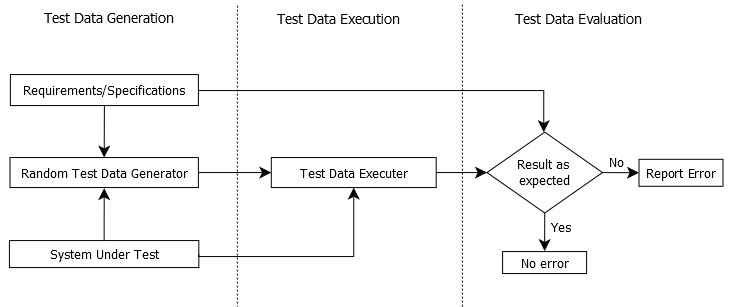
\includegraphics[width=14cm, height=6cm ]{Introduction/SoftwareTesting.png}
		\caption{Three main phases of random testing}
	\label{fig:SoftwareTesting}
\end{figure}

\section{The Problems}
Exhaustive testing of software is not always possible and the problem of selecting a test data set, from a large/infinite domain is often confronted. Test data set, as a subset of the whole domain, is carefully selected for testing the given software. Adequate test data set is a crucial factor in any testing technique because it represents the whole domain for evaluating the structural and/or functional properties~\cite{howden1986}, \cite{mccabe1983}. Miller and Maloney were the first who comprehensively described a systematic approach of test data set selection known as path coverage. They proposed that testers select the test data so that all paths of the SUT are executed at least once \cite{Miller1963}. The implementation of the strategy resulted in higher standards of test quality and a large number of test strategies were developed afterwords including boundary value analysis and equivalence class.

Generating test data set manually is a time-consuming and laborious exercise~\cite{korel1990}; Therefore, automated test data set generation is always preferred. Data generators can be of different types i.e. Path-wise, Goal-Oriented, Intelligent or Random~\cite{wiki2013}. Random generator produces test data set randomly from the whole domain. Unlike other approaches random technique is simple, widely applicable, easy to implement, faster in computation, free from bias and costs minimum overhead~\cite{Ciupa2007}.  According to Godefroid et al, ``Random testing is a simple and well-known technique which can be remarkably effective in discovering software bugs"~\cite{Godefroid2005}.

Despite the benefits of random testing, its simplistic and non-systematic nature exposes it to high criticism~\cite{white1987}. Myers et al.~\cite{Myers2011} mentioned it as, ``Probably the poorest methodology of all is random-input testing...". However, Ciupa et al. reported that the above stated statement is based on intuition and lacks any experimental evidence \cite{Ciupa2008a}. The criticism motivated the researchers to look into various aspects of random testing for evaluation and possible improvement. Adaptive random testing (ART)~\cite{Chen2008}, Restricted Random Testing (RRT)~\cite{Chan2002}, Feedback Directed Random Testing (FDRT)~\cite{Pacheco2007a}, Mirror Adaptive Random Testing (MART)~\cite{Chen2003} and Quasi Random Testing (QRT)~\cite{Chen2005} are a few of the enhanced random testing techniques reported in the literature.

Random testing is also considered weak in providing high code coverage~\cite{cohen1997},~\cite{Offutt1996}. For example, in random testing when the conditional statement  ``{\it if (x == 25) then ... }"  is exposed to execution then there is only one chance, of the ``{\it then...}" part of the statement, to be executed out of $2^\text{32}$. If {\it x} is an integer variable of 32 bit value~\cite{Godefroid2005}. 

Random testing is no exception when it comes to the complexity of understanding and evaluating test results. Modern testing techniques simplify results by truncating the lengthy log files and displaying only the fault revealing test cases in the form of unit tests. Further efforts are required to get the test results of random testing in more compact and user-friendly way. 


\section{Research Goals} \label{ResearchGoals}
The main goal of the research study is to develop new techniques for automated random testing with the aim to achieve the following objectives:

\begin{enumerate}
\item To develop a testing strategy with the capability to generate more fault-finding test data.

\item To develop a testing technique for finding faults, fault domains and presentation of results on a graphical chart within the specified lower and upper bound. 

\item To develop a testing framework with focus on increase in code coverage along with generation of more faultfinding test data. 

\end{enumerate}

\section{Contributions}
The main contributions of the thesis research are stated below: 

\subsection{Dirt Spot Sweeping Random Strategy}
%Development of a new enhanced and improved form of automated random testing: the Dirt Spot Sweeping Random (DSSR) strategy. This strategy is based on the assumption that faults and unique failures reside in contiguous blocks and stripes. The DSSR strategy starts as a regular random+ testing strategy � a random testing technique with preference for boundary values. When a failure is found, it increases the chances of using neighbouring values of the failure in subsequent tests, thus slowly sweeping values around the failures found in hope of finding failures of different kind in its vicinity.
%The DSSR strategy is implemented in the YETI random testing tool. It is evaluated against random (R) and random+ (R+) strategies by testing 60 classes (35,785 line of code) with one million ($10^\text{6}$) calls for each session, 30 times for each strategy. The results indicate that for 31 classes, all three strategies find the same unique failures. We analysed the 29 remaining classes using t-tests and found that for 7 classes DSSR is significantly better than both R+ and R, for 8 classes it performs similarly to R+ and is significantly better than R, and for 2 classes it performs similarly to random and is better than R+. In all other cases, DSSR, R+ and R do not perform significantly differently. Numerically, the DSSR strategy finds 43 more unique failures than R and 12 more unique failures than R+.

The faultfinding ability of the random testing technique decreases when the failures lie in contiguous locations across the input domain. To overcome the problem, a new automated technique: Dirt Spot Sweeping Random (DSSR) strategy was developed. It is based on the assumption that unique failures reside in contiguous blocks and stripes. When a failure is identified, the DSSR strategy selects neighboring values for the subsequent tests. Resultantly, selected values sweep around the failure, leading to the discovery of new failures in the vicinity. Results presented in Chapter~\ref{chap:DSSR} indicated higher faultfinding ability of DSSR strategy as compared with Random (R) and Random+ (R+) strategies.

\subsection{Automated Discovery of Failure Domain}
The existing random strategies of software testing discover the faults in the SUT but lack the capability of locating the fault domains. In the current research study, a fully automated testing strategy named, ``Automated Discovery of Failure Domain (ADFD)" was developed with the ability to find the faults as well as the fault domains in a given SUT and provides visualization of the identified pass and fail domains in the form of a chart. The strategy is described, implemented in YETI, and practically illustrated by executing several programs of one and two dimensions in the Chapter~\ref{chap:ADFD}. The experimental results proved that ADFD strategy automatically performed identification of faults and fault domains along with graphical representation in the form of chart.

\subsection{Invariant Guided Random+ Strategy}
Another random test strategy named, ``Invariant guided Random+ Strategy (IGR+S)�" was developed in the current research study. IGR+S is an extended form of Random+ strategy guided by software invariants. Invariants from the given SUT are collected by Daikon�--- an automated invariant detector for reporting likely invariants and adding them to the SUT as assertions. The IGR+S is implemented in YETI and generates values in compliance with the added assertions. Experimental results presented in Chapter~\ref{chap:IGR+S} indicated improved features of IGR+S in terms of higher code coverage and identification of subtle errors that R, R+ and DSSR strategies were either unable to accomplish or required larger duration.  



 
\section{Structure of the Thesis}
%
The rest of the thesis is organized as follows: In Chapter 2, a thorough review of the relevant literature is given. It includes a brief introduction of software testing techniques followed by automated random testing tools. Chapter~\ref{chap:DSSR} describes Dirt Spot Sweeping Random (DSSR) strategy, which is based on sweeping of fault clusters in the input domain. Chapter~\ref{chap:ADFD} presents the newly developed Automated Discovery of Fault Domains  (ADFD) strategy, which focuses on dynamically finding the faults and domains along with their graphical representation. Chapter~\ref{chap:IGR+S} presents the new strategy Invariant Guided Random+ Strategy (IGR+S) developed with the focus on quick identification of faults and increase in code coverage with the help of assertions. Chapter 6 summarizes contributions of the thesis research, discusses the strength and weaknesses of the study, gives conclusion and suggests avenues for future work. Chapter 7 ?






%Today, the primary focus of software companies is to achieve high quality. These companies spend an estimated thirty to ninety percent of the total software development cost on testing \ref{Beizer1990}, \ref{Standards2002}. In spite of spending 

%Software testing is the process of executing a software with specific test data followed by evaluation of the results to check whether it is working according to its specification or not \ref{Sommerville2006}.
% check here if we can replace specification with oracle or not.
%The test passes if the output complies to its specification and fails otherwise. The success of testing correlates with the number of failures found in the Software Under Test (SUT): a test is more successful if it finds more faults.

%It is interesting that program testing is used to show the presence of bugs, rather than absence of bugs [6]. Therefore the SUT that passes all the tests without returning a single failure does not guarantee that there is no fault. The testing process increases however the reliability and confidence of both the developers and the users in the tested product [7] [8] [9].

%Random testing is a black-box testing technique in which the SUT is executed against ran- domly selected test data. Test results obtained are compared either against the oracle defined, using SUT specifications in the form of assertions or exceptions defined by the programming language. The rapid increase in software development in today?s modern world prompts the need for automated testing to ensure high quality. The generation of random test data is com- paratively cheap and does not require too much intellectual and computation efforts [10] [11]. It is for this reason that various researchers have recommended this strategy for incorporation in automatic testing tools [12]. YETI [13] [14], AutoTest [15] [16], QuickCheck [17], Randoop [18], JArtage [19] are a few of the most common tools based on random strategy.


%%% ----------------------------------------------------------------------


%%% Local Variables: 
%%% mode: latex
%%% TeX-master: "../thesis"
%%% End: 

% These chapters are commented by me for now to quickly render.
%% \pagebreak[4]
% \hspace*{1cm}
% \pagebreak[4]
% \hspace*{1cm}
% \pagebreak[4]
\chapter{Literature Review}
%\ifpdf
%    \graphicspath{{Literature/LiteratureFigs/PNG/}{Literature/LiteratureFigs/PDF/}{Literature/LiteratureFigs/}}
%\else
%    \graphicspath{{Literature/LiteratureFigs/EPS/}{Literature/LiteratureFigs/}}
%\fi




Paul Ehrlich famous quote is, ``To err is human, but to really foul things up you need a computer". Since the programmers are ordinary human beings, it is most obvious that some errors remain in the software after its completion. Errors are not tolerated as they can cause great loss. According to the National Institute of Standard and Technology 2002, 10 report, software errors cost an estimated \$59.5 billion loss to US economy annually. The destruction of the Mariner 1 rocket (1962) that cost \$18.5 million was due to a simple formula coded incorrectly by a programmer. The Hartford Coliseum Collapse (1978) costing \$70 million, Wall Street crash (1987) costing \$500 billion, Failing of long division by Pentium (1993) costing \$475 million, Ariane 5 Rocket disaster costing \$500 million and many others are caused by minor errors in the software. To achieve high quality, the software has to satisfy rigorous stages of testing. The more complex and critical the software, the higher the requirements for software testing and the larger the damage caused if the bug remains in the software. 

\section{Software Testing}
In the IEEE standard glossary of software engineering terminology \cite{american1984}, testing is defined as the process of exercising or evaluating a system or system component by manual or automated means to verify that it satisfies specified requirements and actual results. A successful test is one that finds a fault \cite{Myers2004}, where faults are defined as the errors made by the people during software development \cite{american1984}.

Being an integral part of Software Development Life Cycle (SDLC), the testing process is started from requirements phase since this is the starting point of all the software activities and continue throughout the life of the software. In traditional testing when testers finds a fault in the given SuT, the software is given back to the developers for removing the fault and after its rectification the software is handed back to the testers for retesting. It is important to understand the fact that ``program testing can be used to show the presence of bugs, but never to show the absence of bugs" \cite{Dijkstra1972}. Which means SUT that passes all the tests without giving a single error is not guaranteed to contain no error. The testing process increase however the reliability and confidence of the users in the tested product.


\begin{table}[ht]
%\scriptsize
\caption{Parts of Software Testing \cite{adrion1982validation}, \cite{chilenski1994applicability}, \cite{gaudel2010software}, \cite{richardson1992specification}, \cite{tracey1998automated}} % title of Table
\smallskip
\centering % used for centering table
\begin{tabular}{| l | l | l | l | } % centered columns (4 columns)
\hline

Levels 		&Purpose		 						& Perspective		& Execution 	\\
\hline
1. Unit		&1. Functionality						& 1. White Box		& 1. Static 	\\
2. Integration	&2. Structural							& 2. Black Box		& 2. Dynamic	\\
3. System		&3. Robustness						& 3. Grey Box		&			\\
			&4. Stress								&				&			\\
			&5. Compatibility						&				&			\\
			&6. Performance						&				&			\\



\hline %inserts single line
\end{tabular}
\bigskip
\label{table:addvalues} % is used to refer this table in the text
\end{table}


\subsection{Software Testing Levels}
Unit testing, integration testing and system testing \cite{chilenski1994applicability} are the three main levels of software testing defined in the literature. Unit testing evaluate a small piece of software code called units for faults. These units are combined together to form components and integration testing ensure that the integration points are working properly. Finally the components are combined to form a system and before production system testing is performed to make sure that it works as expected. 


\subsection{Software Testing Purpose}
The primary purpose of software testing is identification of faults in the given SuT so that they can be corrected to achieve high quality. Ideally, maximum number of faults can be identified if software is tested exhaustively i.e. testing SuT against all possible combinations of input data, and comparing the obtained results to the expected results for assessment. However, exhaustive testing is not always possible in most of the test scenarios because of limited resources and infinite number of input values that a software can take. Therefore, the purpose of testing is generally directed to achieve confidence in a specific aspect of a SuT. For example, functionality testing is performed to check if one or more functions of a system are working correct or not. Structural testing analyse the code structure to generate test cases in order to evaluate paths of execution and identification of unreachable or dead code.  In robustness testing the software behaviour is observed in the case when it receive input that is outside of its expected input range.  Stress and performance testing aim to test the response of software under high load and its ability to process different nature of tasks \cite{cohen2005robustness}. Finally, compatibility testing is performed to see the interaction of software with underlying operating system or hardware.
 %As proper planning is the key to success for many projects this is often also true with software testing. A software test plan is a well defined document that defines the goal, scope, method, resources and time schedule of the testing.
%A software testing technique in which a software is tested with all possible combination of inputs. This technique can prove conclusively that the software meet its specification however exhaustive testing is seldom feasible because of the large input domain or too many paths in a software code. 

\subsection{Software Testing Perspective}
Testing activities can be split up into blackbox and whitebox testing on the basis of perspective taken. In blackbox or functional testing the testers dont need to know about internal code structure of the SuT. Test cases are derived from the specifications and test passes if the output is according to expected output. Internal code structure of the SuT is not taken into any consideration \cite{beizer1995black}. Whereas in whitebox or structural testing testers must know about the complete structure of the software and can modify it, if required. Test cases are derived from the code structure and test passes only if the results are correct and the expected code is followed during test execution \cite{ostrand2002white}.

%\subsubsection{Grey-Box Testing}
%Grey-Box testing is the combination of both black-box/functionality and white-box/structural testing. The tester knows about both the functionality and the internal structure of the SUT. Some of the test cases are based on the functionality and some of the test cases are based on the structure. Emphasis of grey-box testing is both on code coverage as well as functionality \cite{Savenkov2008}.

%\subsection{Software Testing Workflow}
%There are many software techniques like unit testing, integration testing, random testing, regression testing, system testing, acceptance testing, performance testing, load testing, stress testing, alpha testing, beta test etc. All testing techniques belong to black-box, white-box or grey-box approach. Each testing technique has its own strength and weaknesses but the technique in focus here is Random Testing.


%\begin{figure}[h]
%\begin{center}
%	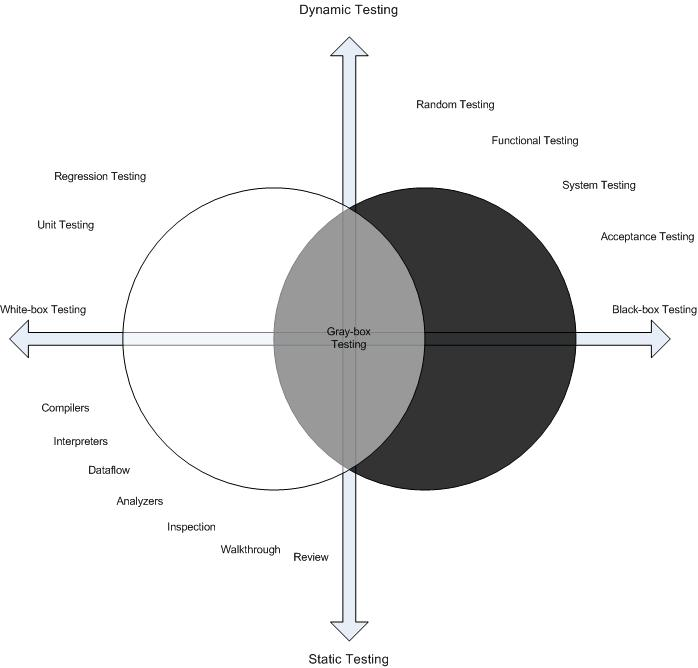
\includegraphics[width=16cm, height=12cm ]{Literature/Drawing34.jpg}
%	\caption{Software Testing Workflow}
%\end{center}  
%\end{figure}


%We have explained software testing graphically with the help of plotting venn diagram on two dimensional axis. The positive x axis represent black-box while negative x axis represent white-box testing. Grey-box testing in the middle is represented by the overlapping of black-box and white-box testing. Similarly on positive y axis we have dynamic testing and on negative y axis we have static testing.
%Now if a test is black box and dynamic then the test will fall in 0 to 90 degree on the diagram and if the test is black-box and static then it will fall in 270 to 360 degree. On the other hand if the test is white-box and dynamic then it will fall in 90 to 180 degree and if the test is white-box and static then it will fall in 180 to 270 degrees.




\subsection{Software Testing Execution}
Test activities can be organised into static and dynamic testing on the basis test cases execution. In static testing test cases analysed statically checked for errors without any execution. All high quality softwares are accompanied by documentation in addition to software code. These include requirements, design, technical, end-user and marketing documentation. Reviews, walkthroughs or inspections are most commonly used techniques for static testing. In dynamic testing the software code is executed and input is converted into output through processing. Results are analysed against expected results to find any error in the software. Unit testing, integration testing, system testing, and acceptance testing are most commonly used as dynamic testing methods \cite{fairley1978tutorial}

%Dynamic testing can be manual or automated. In manual testing the programmer develops the test cases which are executed by the developed software to find any error in processing or output. Similarly in automated testing the software or components of the software is given as input to testing software that automatically generates test cases and executes the SUT against them to find any errors. Manual testing typically consumes more time and resources than automated testing.



\subsection{Manual Testing}
 A software testing technique to find faults in a class or group of related classes, such that the tester must write the code by hand to create test cases and test oracle \cite{Ciupa2008}. While manual testing is effective in some cases, in general, it is a laborious, time consuming, error-prone \cite{tretmans1999}. It further requires testers to have appropriate skills, experience and in depth knowledge of the under test software in order to evaluate it from different perspectives.
 
\subsection{Automated Testing}
A software testing technique to find faults in a class or group of related classes, such that the test cases and test oracle is generated automatically by a testing tool \cite{Leitner2007}. The tools can automate part of a test i.e. generation of test cases, execution of test cases and evaluation of results or the whole test process. The use of automated testing made it possible to test large volumes of code that would be otherwise impossible \cite{ramamoorthy1975}.

%\section{Automated Random Testing}
%\subsection{Test Data Generation}
%\subsection{Test Execution}
\subsection{Test Oracle}
Test oracles set the acceptable behaviour for test executions \cite{richardson1992specification}. All softwares testing techniques depend on the availability of a test oracle \cite{baresi2001test}. Designing test oracles for simple softwares may be straight forward, however, for relatively complex softwares it can be very cumbersome to decide whether a program execution returns a correct or incorrect result \cite{gaudel2010software}. Different testing techniques tackle the oracle problem in various ways but some of the common issues include:
\begin{enumerate}
\item It is assumed that execution results are observable, so that they can be evaluated against the test oracle or the oracles are defined on the basis of these results.
\item An ideal test oracle would satisfy desirable properties of program specifications \cite{baresi2001test}.
\item There is not a single oracle generation technique that satisfies all purposes. Weyuker \cite{weyuker1982testing} argued that truly general test oracles are often unobtainable.
\end{enumerate}
%\subsection{Test Report}

\subsubsection{Random Testing}
Random testing is a dynamic and black-box testing technique in which the software is tested with non-correlating or unpredictable test data from the specified input domain \cite{Chan2002}. The input domain is a set of all possible inputs to the software under test. According to Richard H. \cite{hamlet1994}, to conduct random testing, an input domain is defined, then test points are randomly taken from the whole input domain through a random number/test case generator. The program under test is executed on these points and the results obtained are compared to the program specifications. The test fails if any input leads to incorrect results or otherwise it is successful. 

\begin{figure}[h]
	\centering
	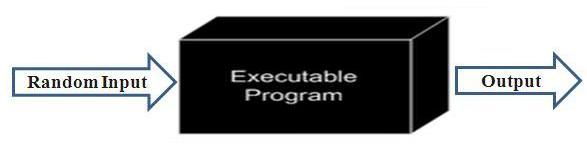
\includegraphics[scale=0.5]{Literature/figure1.jpg}
	\caption{Random Testing}
\end{figure}

It is quick and cheap to generate random test data as it don't require too much intellectual and computational efforts \cite{Ciupa2009}. This capability makes it an ideal choice for implementation in automated testing tools \cite{Ciupa2008a}. In addition, no human intervention in data generation/selection makes it one of the most unbiased testing technique. 

Generating test cases with out using any background information makes it highly susceptible to criticism. Myers \cite{Myers1979} intuitively mentioned random testing as one of the least effective testing technique. It is also criticised for generating many sets of tests that lead to the same state of the software. Furthermore, random testing can generate test inputs that violates requirements of the given SUT making it less effective \cite{sen2007effective}, \cite{pacheco2009directed}. 

Myers statement was not based on any experimental evidence and later on the experiments performed in \cite{hamlet1994}, \cite{Ciupa2008}, \cite{leitner2007efficient} and \cite{Duran1981} confirmed that random testing is as effective as any other systematic testing technique. The experiments in \cite{Duran1981} found that random testing can find subtle faults in a given SUT if run for large number of test cases. They argued that the simplicity and cost effectiveness of random testing can make it feasible to run large number of test cases as opposed to systematic testing which requires considerable time and resources for test case generation and execution. The empirical comparison \cite{hamlet1990} also prove that random testing and partition testing are equally effective. Furthermore the study conducted by Ntafos \cite{ntafos1998random} conclude the effectiveness of random testing over proportional partition testing.



\section{Variations in Random Testing}
Different researchers tried various strategies to improve the performance of random testing. In order to better understand the topic we have studied each strategy in detail.

\subsection{Adaptive Random Testing}
Adaptive random testing (ART) \cite{Chen2008} is based on the existence of failure patterns across the input domain detected by Chan et al \cite{Chan1996}. They observed that failure inducing inputs in the whole input domain form certain geometrical patterns. They divided these patterns into point, block and strip fault patterns. Each one is described below.

\begin{figure}[h]
	\centering
	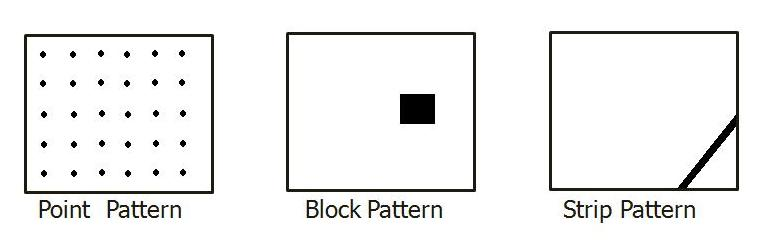
\includegraphics[scale=0.5]{Literature/pointblockstrip}
	\caption{Patterns of failure causing inputs}
	\label{fig:patterns}
\end{figure}

In the figure \ref{fig:patterns} the square box indicates the whole input domain. The white space shows legitimate or faultless values while the black colour points, block and strip inside each box indicate the point, block and strip fault patterns in the input domain.

\begin{enumerate}
\item Point pattern: In the point pattern failure inducing inputs are scattered across the input domain in the form of stand-alone points. Example of point pattern is the division by zero in a statement total = num1/num2; where num1, num2 and total are variables of type integer. 
\item Block pattern: In the block pattern multiple failure inducing inputs lies in a close vicinity to form a block in the input domain. Example of block pattern is failure caused by a statement if ( (num \textgreater 10) \&\& (num \textless 20) ). Here 11 to 19 is a block of faults.
\item Strip pattern: In the strip pattern the failure inducing inputs form a strip across the input domain. Example of strip pattern is failure caused by a statement num1 + num2 = 20. Here multiple values of num1 and num2 can lead to the fault value 20.
\end{enumerate}

The authors argued that ordinary random testing may generate test inputs lurking too close or too far from the fault inducing input and thus failing to discover it. To generate more fault targeted test inputs they suggested ART. ART is a modified version of ordinary random testing where test values are selected at random like before but evenly spread across the input domain. To achieve an even distribution of test cases across the input domain they used two sets. The executed set having the test cases that have been executed by the system and the candidate set that contain the random selected test cases from the bounded input domain as candidates for execution. Initially both the sets are kept empty. The first test case is selected at random from the candidate set and stored in executed set after execution, the second test case is then selected from the candidate set based on the criteria that it is far away from the last executed test case. Thus the whole input domain can be tested and their are more chances of generating test input from inside of the existing geometrical patterns. 

In the experiments they used number of test cases required to detect first failure (F-measure) as a performance matrix instead of the traditional matrix i.e. probability of detecting at least one failure (P-measure) and expected number of failures detected (E-measure). Results of the experiments performed on published programs using ART showed up to 50\% increase in the performance of than ordinary random testing. Results showed significant improvement, however, the issues of increase overhead, spreading test cases across the input domain for complex objects and efficient ways of selecting candidate test cases still exist. Chen et al evolve their work on ART to address some of these issues in \cite{chen2009enhanced} and \cite{Chen2005}. 

\subsection{Mirror Adaptive Random Testing}
As discussed in the above section ART provide better results, however the increase in overhead due to extra computation to achieve even spread of test inputs makes it less cost effective. Mirror Adaptive Random Testing (MART) \cite{Chen2003} is an innovative approach that uses mirror partitioning technique to reduce the overhead of ART by decreasing the extra computation involved in ART.

\begin{figure}[h]
\begin{center}
	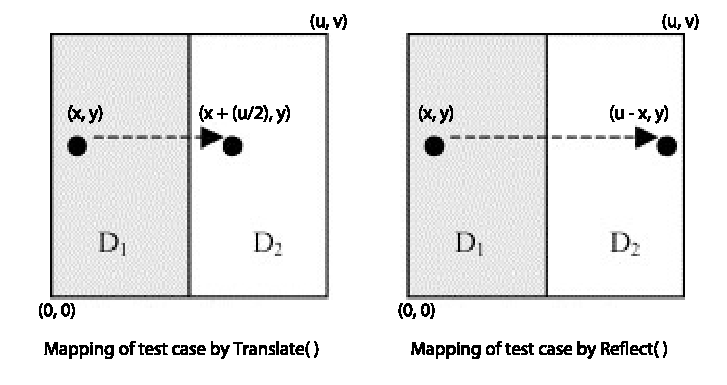
\includegraphics[width=13cm, height=6cm ]{Literature/mart2.pdf}
	\caption{Mirror Adaptive Random Testing \cite{Chen2003}}
\label{fig:mirrorART}
\end{center}  
\end{figure}

In this technique, the input domain of the program under test is divided into n disjoint subdomains of equal size and shape. One of the subdomain is called source subdomain while all the others are termed as mirror subdomains. ART is then applied only to the source subdomain to select the test cases and from all other subdomains test cases are selected by using mirror function. In MART \{(0, 0), (u, v)\} are used to represent the whole input domain where (0, 0) are the leftmost and (u, v) are the rightmost top corner of the two dimensional rectangle. On splitting it into two subdomains we get \{(0, 0), (u/2, v)\} as source subdomain and \{(u/2, 0), (u, v)\} as mirror subdomain. Let suppose we get x and y test cases by applying ART to source subdomain, now we can linearly translate these test cases to achieve the mirrored effect, i.e. (x + (u/2), y) as shown in the figure \ref{fig:mirrorART}. Experimental results showed that the performance of MART is equal to ART with MART using only one quarter of the calculations of that of ART.    


\subsection{Restricted Random Testing}
Restricted Random Testing (RRT) \cite{chan2003normalized} is another approach, with small overhead in contrast to ART, to spread the the test cases more evenly across the input domain. RRT achieves this by creating a circular exclusion zone around the executed test case. A candidate is randomly selected from the input domain for the next test case. Before execution the candidate is checked and is discarded if it lies inside the exclusion zone. This process repeats until a candidate laying outside the exclusion zone is selected. This ensures that the test case to be executed is well apart from the last one. The radius of exclusion zone is constant around each test case and the area of each zone decreases with successive cases.

\begin{figure}[h]
	\centering
	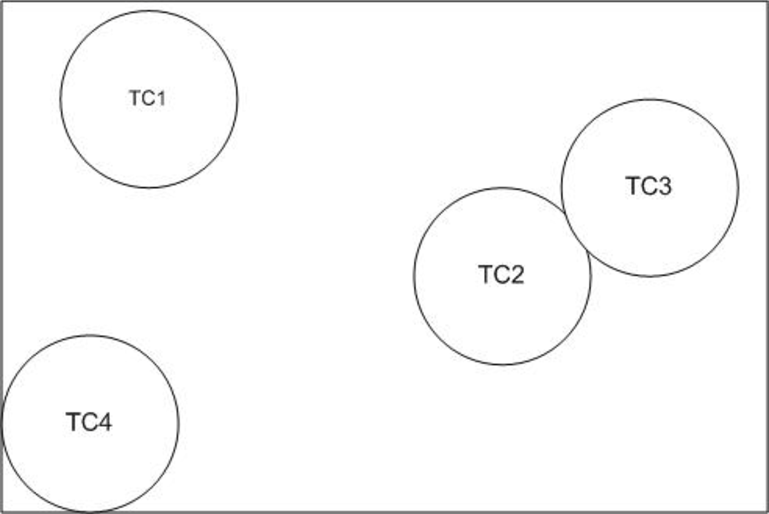
\includegraphics[width= 6cm, height = 5cm]{Literature/RRT.pdf}
	\caption{Input domain with exclusion zone around the selected test case}
\end{figure}

To find the effectiveness of RRT, the authors compared it with ART and RT on 7 out of the 12 programs evaluated by ART and MART. The experimental results showed that the performance of RRT increases with the increase in the size of the exclusion zone and reaches to maximum when the exclusion zone is raised to largest possible size. Normalized Restricted Random Testing \cite{chan2003normalized} is an improvement over RRT by allowing the testers to have better information about the target exclusion rate (R) of RRT. They further found that RRT is up to 55\% more effective than ordinary random testing in terms of F-measure (Where F-measure is the total number of test cases required to find the first failure).



\subsection{Directed Automated Random Testing}


\subsection{Quasi Random Testing}
Quasi-random testing (QRT) \cite{Chen2005} is a testing technique that takes advantage of failure region contiguity by distributing test cases evenly similar to ART but with decreased computation. Chan et al after the analysis of faults in various experiments found that the fault patterns across the input domain are continuous. To achieve even spreading of test cases, QRT uses a class with a formula, that forms an s-dimensional cube in s-dimensional input domain and generate sequence of numbers that have small discrepancy and low dispersion. These sequence of numbers are then used to generate random test cases that are permuted to make them less clustered and more even than RT. An empirical study was conducted to compare the effectiveness of QRT with ART and RT. The 12 numerical programs picked for experiments were the same used to evaluate ART.The empirical results of the experiments showed that in 9 out of 12 programs QRT on average finds a fault quickly than ART and RT while in the remaining three programs the improvement is insignificant.
%\subsection{Monti Carlo Random Testing}

%\subsection{Good Random Testing}

\subsection{Feedback-directed Random Testing}
Feedback-directed Random Testing (FDRT) \cite{Pacheco2007} is a technique that generate unit test suite at random for object oriented programs. As the name implies FDRT uses the feedback received from the execution of first batch of randomly selected unit test suite to generate next batch of more directed unit test suite. In this approach redundant and illegal unit tests are eliminated incrementally from the test suite with the help of filtration and application of contracts. For example unit test that produce IllegalArgumentException on execution is discarded, because, randomly selected argument used in this test was not according to the type of argument the method required.

\subsubsection{Randoop: Feedback-directed Random Testing}
The FDRT technique is implemented in RANDOOP tool \cite{Pacheco2007b}. RANdom tester for Object Oriented Programs (RANDOOP) is a fully automatic tool, capable of testing Java classes and .Net binaries. RANDOOP takes as input a set of classes (java or .Net executables), contracts, filters and the time limit after which the testing process stops. Its output is a suite of JUnit and NUnit for Java and .Net programs respectively. Each unit test in a test suite is a sequence of method calls (hereafter referred as sequence). RANDOOP build the sequence incrementally by randomly selecting a public method from the class under test and arguments for these methods are selected from the predefined pool in case of primitive types and a sequence or null value in case of reference type. RANDOOP maintains two sets called ErrorSeqs and NonErrorSeqs to record the feedback. It extends ErrorSeqs set in case of contract or filter violation and NonErrorSeqs set if no violation is recorded in the feedback. The use of this dynamic feedback evaluation at runtime bring an object to very complex and interesting state. On test completion it produce ErrorSeqs and NonErrorSeqs as JUnit/NUnit test suite. To find the effectiveness of the strategy, in terms of coverage and number of faults discovered, the authors compared RANDOOP implementing FDRT with random testing of JCrasher and JavaPathFinder \cite{visser2004test}. In the experiments 14 libraries of both Java and .Net were evaluated.  The results showed that RANDOOP achieved more coverage than JCrasher in behavioural, branch coverage and faults detection. It can achieve on par coverage with systematic approaches like JavaPathFinder. RANDOOP also has an edge over model checking for its ability to easily search large input domains.
%\subsection{Adaptive Random Testing for Object-Oriented}



\subsection{Object Distance and its application}
To improve the performance of random testing the emphasis of ART was on the distance between the test cases. But this distance was defined only for primitive data types like integers and other elementary input. Ciupa et al defined the parameters that can be used to calculate distance between the composite programmer-defined types so that ART can be applicable to testing of todays object-oriented programs \cite{Ciupa2006}. Two objects have more distance between them if they have more dissimilar properties.
The parameters to specify the distance between the objects are dynamic types, values of its primitive and reference fields. Strings are treated as a directly usable values and Levenshtein distance \cite{Levenshtein1966} which is also known as edit distance is used as a distance criteria between the two strings.
To implement object distance first all the distances of the objects are measured. Then two sets candidate- objects containing the all the objects ready to be run by the system and the used-objects set which is initially empty. First object is selected randomly from the candidate-object set and is moved to used- object set when executed by the system. Now the second object selected from the candidate set for execution is the one with the biggest distance from the last executed object present in the used-object set. This process is continue until the bug is found or the objects in the candidate-object set are finished.

\subsubsection{ARTOO Tool}
After the criteria to calculate the distance between the objects is defined \cite{Ciupa2006}, the same team implemented that model and performed several experiments to evaluate the proposed model. Adaptive Random Testing for Object Oriented (ARTOO) is a testing strategy, based on object distance, implemented in AutoTest tool [16].
ARTOO was implemented as a plug-in strategy in AutoTest. It only deals with creating and selecting inputs and all other functionality of the AutoTest was the same. Since ARTOO is based on object distance therefore the method for test input selection is to pick that object from the candidate set (A pool of objects that is a potential candidate to be executed by the system) which has the highest average distance in comparison to the objects already executed.
In the experiments classes from EiffelBase library [17] were used. To evaluate ARTOO the same tests were also applied to directed random strategy (RAND). The outcome of the experiments showed that ARTOO finds the first bug with fewer test cases than RAND. The computation to select test case in ARTOO is more than RAND and therefore ARTOO takes more time to generate a test input. The experiments also found few of the bug found by ARTOO were not pointed out by RAND furthermore ARTOO is less sensitive to the variation of seed value than RAND.

\subsubsection{Experimental Assessment of RT for Object-Oriented Software}
In this research the effect of various parameters involved in random testing and its effect on efficiency is evaluated by performing various experiments on Industrial-grade code base.
Large scale clusters of computers were used for 1500 hours of CPU time which resulted in 1875 test sessions for 8 classes under test. \cite{Ciupa2007} The finding of the experiments are
1. Version of random testing algorithm that is efficient for smaller testing timeout is equally efficient for higher testing timeouts.
2. The value of seed for random testing algorithm plays a vital role in finding the number of bugs in specific time.
3. Most of the bugs are found in the first few minutes of the testing sessions.


%\section{Automated Random Testing Tools}

\subsection{JCrasher}
JCrasher is an automatic testing tool that uses a random testing technique to test java classes/programs \cite{Pacheco2007b}. The main features of JCrasher are:
1. The randomly created test cases are according to the type and parameters of the methods under test.
2. It uses special heuristics rules, after the execution of the test cases, to see whether the given excep- tions are real bugs or the generated input violated the pre-conditions of the program.
3. To clarify the testing from any old tests JCrasher make it sure that every test run on a clean state.
4. JCrasher also produces test cases for JUnit that can be integrated into IDEs like Eclipse.
To use JCrasher we have to supply set of Java classes in byte code and testing time. JCrasher analyzes the classes and create test cases randomly with the same type and same parameter list. These test cases are only for public methods of the classes and they check for any system crash. List of exceptions is obtained as a result of execution of test cases which are differentiated as bugs and precondition violations by the input.

\subsection{JArtage}
Jartege (JAwa Random TEst GEnerator) is a tool that randomly generates unit tests for classes specified with JML (Java Modeling Language) \cite{Oriat2004}. The specification of Java classes with JML serves two pur- poses. First, all the test cases generated by Jartege have to verify the conditions defined by JML and thus irrelevant test cases are eliminated. Secondly these JML specifications are also used as oracles. Apart from the JML specification which are made by hand it automates the whole testing process which include test case generation, execution, comparing it against oracle and using the generated test cases for future regression testing.

\subsection{Eclat}
Eclat \cite{Pacheco2005} is a tool that automatically generates unit tests for Java. Eclat can be executed from both command line or from IDE where it can be installed as a plug-in. [28]. Eclat selects a sub-set of test inputs from a large domain, that is likely to reveal fault in the SUT. Eclat takes a correct execution of the SUT and on the basis of it creates an operational model. It then selects only these test inputs from the input domain which fail to comply with the model. A Reducer function removes the redundant test inputs and the remaining test inputs are likely to discover faults in the SUT. Based on the operational model it also produces an automated oracle. Various experiments results shows that Eclats is very effective in finding faults and the ratio of finding faults and test inputs is almost same.

\subsection{JTest}
Parasoft Jtest is a commercial tool that automatically generates and execute unit tests. It can be easily integrated to Java IDEs like Eclipse where it provide two main functionalities, i.e. Static Analysis, Unit testing and code coverage. [25]
In static analysis Jtest takes a complete project or set of classes as input and compares it with a list of built-in rules. The statement violating any of these rules is an error. It also suggests probable fixes for the detected fault.
For unit testing it takes a class as an input and processes a number of scenarios against it to generate and execute unit tests. Once unit tests are executed they become the part of regression test for future reference.
Jtest also shows the code coverage of the program by colour coding the statements that are not executed by the unit tests.

\subsection{QuickCheck}
QuickCheck \cite{Claessen2000} is a light weight random testing tool that is developed specifically for testing of Haskell programs \cite{Hudak2007}. Haskell is a functional programming language where programs are evaluated using expressions rather than statements as in case of imperative programming. Therefore in this process the tester defines certain expressions for the functions that must hold for a large number of test cases to be correct. These test cases are generated automatically through generator function which can be set by the tester to generate random test cases or according to specific criteria. After processing all the generated test cases any test case that causes the expression to become false is considered faults.

\subsection{AgitarOne}
AgitarOne is a commercial tool that automatically generates unit tests. It has a Junit Generator engine that can create 25,000 lines or more of Junit per hour [29]. It can be easily integrated into famous IDE like Eclipse. It takes as input, classes under test, time and optionally any knowledge or test cases that has a positive influence on the performance of the testing process. The generated Junit tests can be run from the same IDE and can also be used for later regression testing. The GUI interface is called a dashboard which provides in depth knowledge of the tests conducted, failures detected, alerts and the archieves of the tests conducted earlier. It also shows the coverage obtained after executing the Junits against the code under test.

\subsection{Autotost}
Based on Formal Automated testing AutoTest is a tool used for testing of Eiffel programs \cite{Ciupa2007}. The Eiffel language use the concept of contracts (pre-conditions, postconditions and class invariants). Input can be a single class, method or a set of classes which is then processed by AutoTest to generate test cases. It generates both primitive and object type test cases. All the generated test cases are kept in a pool and then randomly a test case is selected from it for execution. A user can set the features of the AutoTest options include: Number of test cases to generate, whether to monitor pre or post condition, order of testing and the initial values of the primitives variables.

\subsection{TestEra}
TestEra \cite{Khurshid2004} is a novel framework for testing Java applications. All the tests are produced and executed in an automated fashion. Tests are conducted on the basis of the method specifications \cite{Chang1999}. TestEra takes methods specifications, integer value as a limit to the generated test cases and the method under test. It uses pre-conditions of a method from specifications to automatically generate test cases up to the specified limit. These test cases are then executed on the method and the result is compared against the postconditions (oracle) of that method. Any test case that fails to satisfy postcondition is considered as a fault. The complete error log is displayed in the Graphical User Inteface (GUI).

\subsection{Korat}
Korat \cite{Boyapati2002} is an automated testing tool for Java programs that generates and execute test cases for a method based on its formal specification. To generate test cases for a method Korat makes use of its pre-condition. It then executes the generated test cases against the method specifications. Korat uses JML for specifications. In order to generate test cases for a method Korat constructs new methods that return a Boolean value (Java Predicate) from its pre-conditions. When given these Java predicates Korat generates all non isomorphic input for which the return value of predicate is true. To check correctness of the method, Korat executes the test cases on that method and analyzes the output with the post conditions of the method (oracle). A fault in a method under test throws an exception to indicate the violation of the post-condition.

\subsection{YETI}
York Extensible Testing Infrastructure (YETI) is an automated tool for testing Java, JML and .NET assemblies \cite{Oriol2010c}. YETI execute the program under test with random generated but type-correct inputs and declare a fault if the response is an unexpected exception or a contract violation. YETI has been designed with an emphasis on extensibility. Its three main parts: the core infrastructure, strategies and language bindings are loosely coupled to easily accommodate new languages and strategies. To keep the process fully automated YETI uses two approaches for oracle (pass/fail judgement). If available, YETI uses code contracts as oracle if not it uses undeclared runtime exceptions of the underlying language as oracle. The test cases revealing errors are reproduced at the end of each test session for unit and regression testing. Other prominent features of YETI include its Graphical User Interface (GUI) for user friendliness and ability to distribute large testing tasks in cloud for parallel execution \cite{Oriol2010}. The following sections briefly describe internal working and execution of YETI tool. 

\subsection{Construction of Test Cases}
YETI construct test cases at random by creating objects of the class under test and randomly calling its methods with inputs according to its parameter's-space. Strategy section contains seven different strategies and inputs to the tested methods is defined by one of the selected strategy. To completely automate the data generation YETI   split input values into two types i.e. primitive data types and user defined classes. For Java primitive data types, which includes short, byte, char, int, float, double, long etc, YETI uses its own built-in random value generation library. However, in the case of user defined classes where objects data type is a user defined class YETI calls its constructor to generate object of that class at run time. It may be possible that the constructor require another object and in this case YETI will recursively calls the constructor of that object. This process is continued until the an object with blank constructor, constructor with only primitive types (type 1) or the set level of recursion is reached. 

\subsection{Commnad-line Options}
While YETI GUI launcher has been developed during this research study, to take maximum benefit of the available options one still need to launch YETI from CLI mode. These command-line options are case insensitive and can be provided as input to the tool in CLI mode. For example, to save processing power command line option -nologs can be used to bypass realtime logging. The following table describes few of the most common command-line options available in YETI.    

\begin{table}[h]
%\scriptsize
\caption{YETI command line options} % title of Table
\smallskip
\centering % used for centering table
\begin{tabular}{ll } % centered columns (4 columns)
\hline

Levels 					&Purpose 			\\
\hline
-java						&Test programs coded in Java	 	\\
-jml						&Test programs coded in JML			\\
-dotnet					&Test programs coded in .NET		\\
-ea						&To check code assertions \\
-nTests					&Specify number of tests after which the test stops	\\
-time						&Specify time in seconds or minutes after which the test stops\\
-testModules				&Specify one or more modules to test 	\\
-rawlogs					&Prints real time logs during test \\
-nologs					&Omit real time logs and print end result only\\
-yetiPath					&Specify path to the test modules\\ 
-gui						&Show test session in GUI\\
-DSSR					&Specify Dirt Spot Sweeping Random strategy for this session\\
-ADFD					&Specify Automated Discovery of Failure Domain strategy for this session\\
-random					&Specify random test strategy for this session\\
-randomPlus				&Specify random plus test strategy for this session\\
-randomPlusPeriodic		&Specify random plus periodic test strategy for this session\\
-nullProbability				&Specify probability of inserting null as input value\\
-newInstanceProability		&Specify probability of inserting new object as input value\\

\hline %inserts single line
\end{tabular}
\bigskip
\label{table:cliOptions} % is used to refer this table in the text
\end{table}


\subsection{YETI Execution}
YETI being developed in Java is highly portable and can easily run on any operating system with Java Virtual Machine (JVM). YETI can be executed from both command line and GUI. To build and execute YETI, it is necessary to specify the project and all the .jar library files particularly javassist.jar in the CLASSPATH or JVM would not be able to find and execute it. There are several options available as discussed in section xxx??? to accommodate specific needs but the typical command to invoke YETI is given in figure \ref{fig:XXX???}. In this particular command YETI tests java.lang.String and yeti.test.YetiTest modules, for details of other options please see section xxx????. 

\begin{figure}[h]
	\centering
	\frame{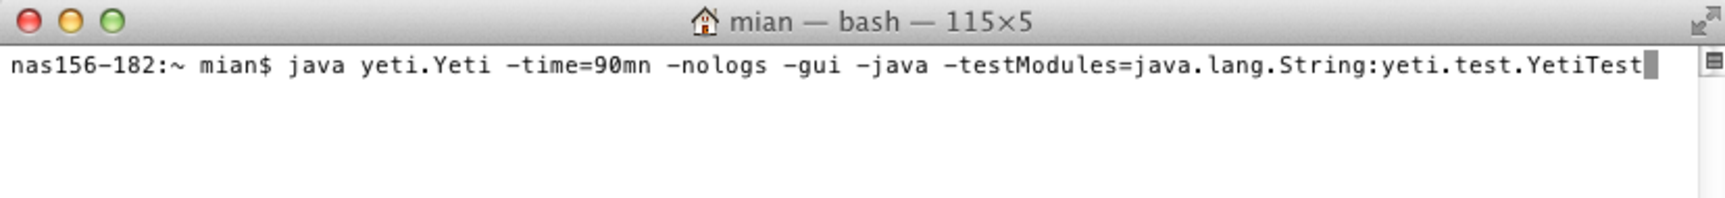
\includegraphics[width= 14cm, height = 1.8cm]{Literature/yetiCommandCLI.pdf}}
	\caption{Command to launch YETI from CLI}
\end{figure}

Alternately, runnable jar file by the name YetiLauncher is also available to launch YETI from GUI. However, till the writing of this thesis, the GUI version of YETI only supports the basic options of YETI. Figure xxx??? shows the equivalent of above command in GUI mode.

\begin{figure}[h]
	\centering
	\frame{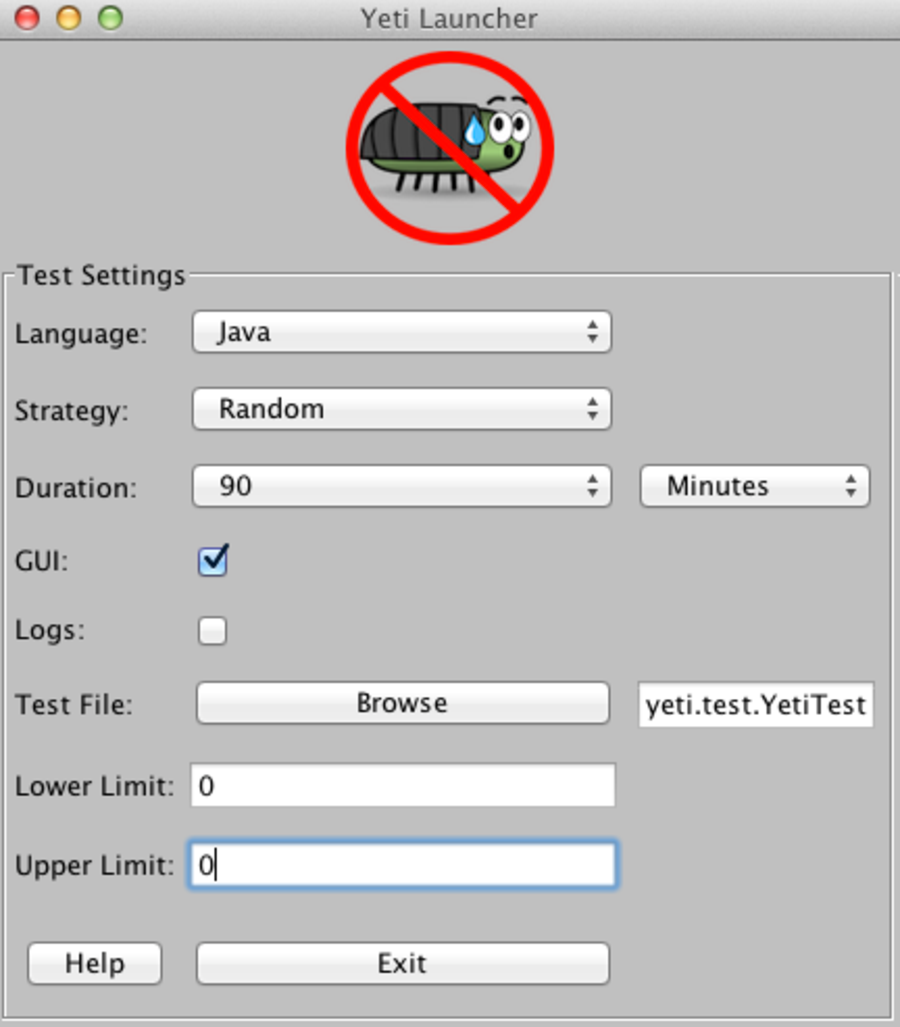
\includegraphics[width= 7cm, height = 8cm]{Literature/yetiCommandGUI.pdf}}
	\caption{Command to launch YETI from GUI}
\end{figure}


As a result of both the above commands YETI launch its own GUI window and start testing the assigned programs. 




\subsection{YETI Report}



\subsection{Tools for Automated Random Testing}
From the literature we can find a number of open source and commercial testing tools that automatically generate unit tests. Each tool utilize different generation technique but the one we are interested in is random technique. We present the most well known tools.

\begin{figure}[h]
	\centering
	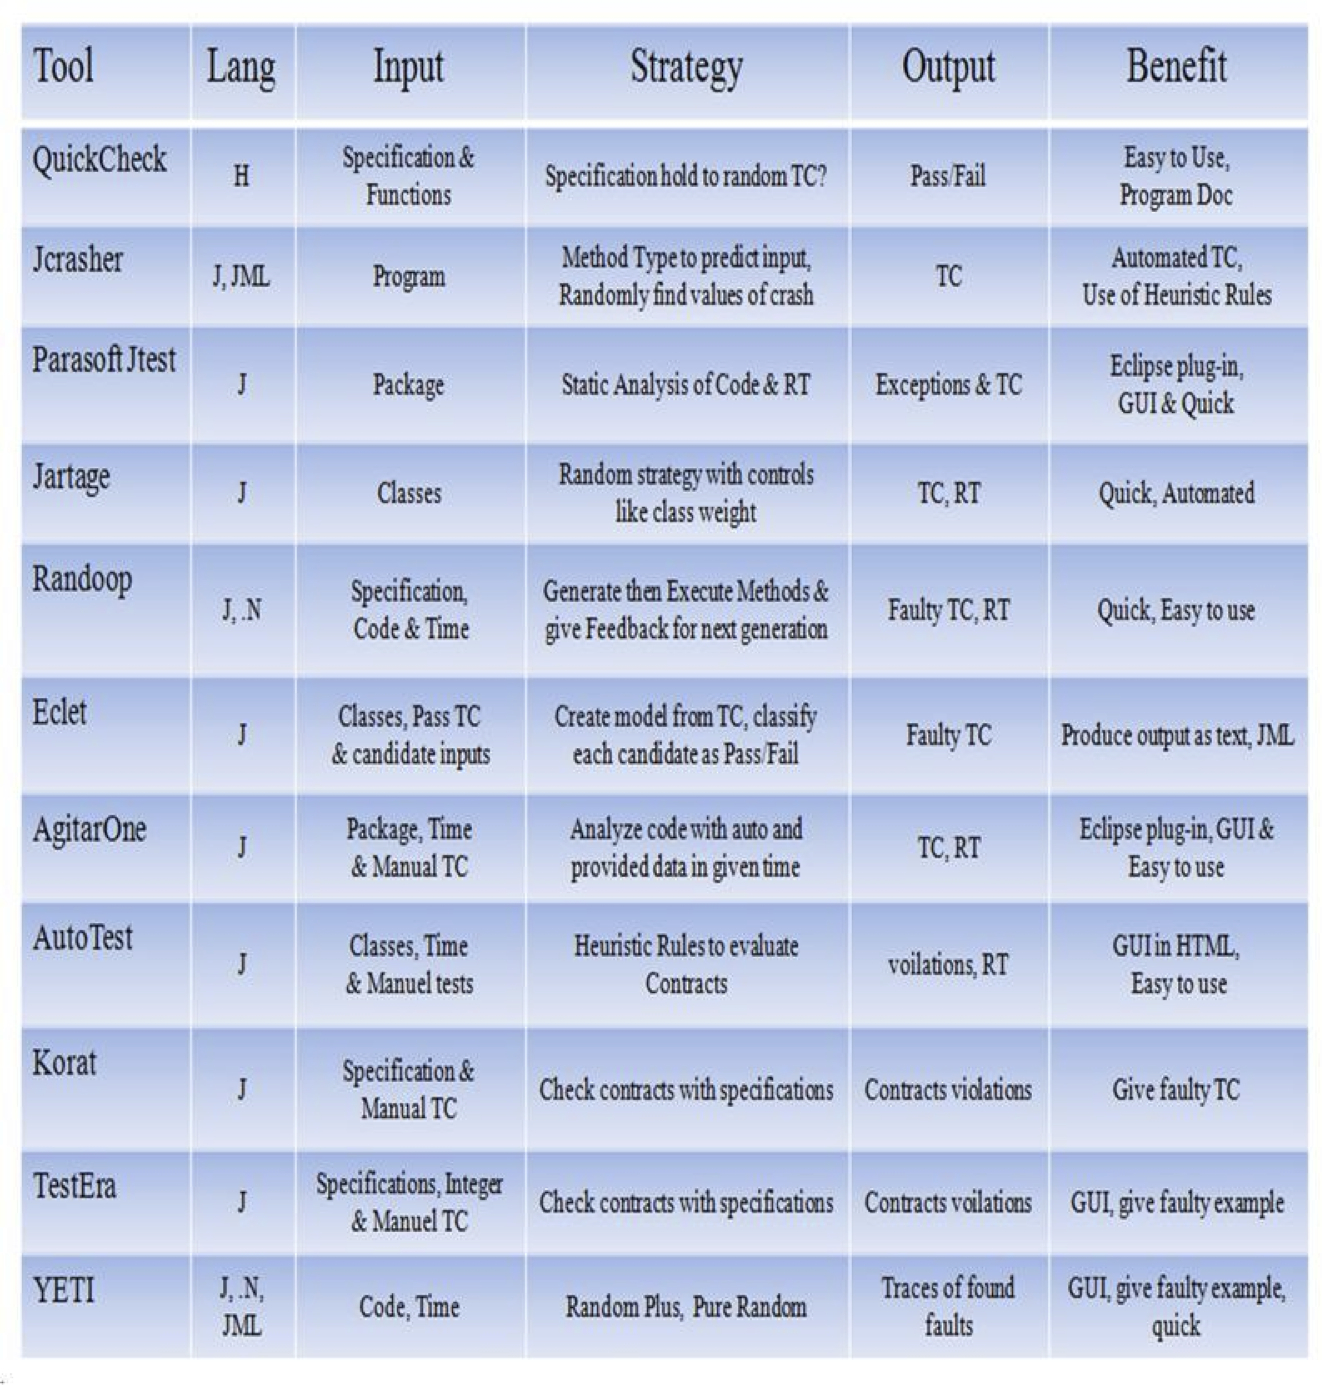
\includegraphics[scale=0.6]{Literature/tools}
	\caption{Summary of automated testing tools}
\end{figure}


\section{Conclusion}


% ------------------------------------------------------------------------


%%% Local Variables:
%%% mode: latex
%%% TeX-master: "../thesis"
%%% End:

%\chapter{Dirt Spot Sweeping Random Strategy}
\label{chap:DSSR}
%\ifpdf
%    \graphicspath{{Dssr/DssrFigs/PNG/}{Dssr/DssrFigs/PDF/}{Dssr/DssrFigs/}}
%\else
 %   \graphicspath{{Dssr/DssrFigs/EPS/}{Dssr/DssrFigs/}}
%\fi

%%%%%%%%%%%%%%%%%    INTRODUCTION   %%%%%%%%%%%%%%%%%%%%
\section{Introduction}\label{sec:intro3}
The success of a software testing technique is mainly based on the number of faults it discovers in the Software Under Test (SUT). An efficient testing process discovers the maximum number of faults in a minimum possible time. Exhaustive testing, where software is tested against all possible inputs, is mostly not feasible because of the large size of the input domain, limited resources and strict time constraints. Therefore, strategies in automated software testing tools are developed with the aim to select more fault-finding test input from input domain for a given SUT. Producing such targeted test input is difficult because each system has its own requirements and functionality.

Chan et al.~\cite{Chan1996} discovered that there are patterns of failure-causing inputs across the input domain. They divided the patterns into point, block and strip patterns on the basis of their occurrence across the input domain. Chen et al.~\cite{Chen2008} found that the performance of random testing can be increased by slightly altering the technique of test case selection. In adaptive random testing, they found that the performance of random testing increases by up to 50\% when test input is selected evenly across the whole input domain. This was mainly attributed to the better distribution of input which increased the chance of selecting inputs from failure patterns. Similarly Restricted Random Testing \cite{Chan2002}, Feedback directed Random Test Generation \cite{Pacheco2007a}, Mirror Adaptive Random Testing \cite{Chen2003} and Quasi Random Testing \cite{Chen2005} stress the need for test case selection covering the whole input domain to get better results.

In this paper we take the assumption that for a significant number of classes failure domains are contiguous or are very close by. From this assumption, we devised the Dirt Spot Sweeping\footnote{The name refers to the cleaning robots strategy which insists on places where dirt has been found in large amount.} Random (DSSR) strategy  which starts as a random+ strategy --- a random strategy focusing more on boundary values. When a new failure is found, it increases the chances of finding more faults using neighbouring values. As in previous studies~\cite{oriol2012law} we approximate faults with unique failures. Since this strategy is an extension of random testing strategy, it has the full potential to find all unique failures in the program, but additionally we expect it to be faster at finding unique failures, for classes in which failure domains are contiguous, as compared with random (R) and random+ (R+) strategies.

We implemented the DSSR strategy in the random testing tool YETI\footnote{\url{http://www.yetitest.org}}. To evaluate our approach, we tested 30 times each one of the 60 classes of 32 different projects from the Qualitas Corpus\footnote{\url{http://www.qualitascorpus.com}} with each of the three strategies R, R+ and DSSR. We observed that for 53\% of the classes all three strategies find the same unique failures, for remaining 47\% DSSR strategy perform up to 33\% better than random strategy and up to 17\% better than random+ strategy.
We also validated the approach by comparing the significance of these results using t-tests and found out that for 7 classes DSSR was significantly better than both R+ and R, for 8 classes DSSR performed similarly to R+ and significantly better than R, while in 2 cases DSSR performed similarly to R and significantly better than R+. In all other cases, DSSR, R+ and R do not seem to perform significantly differently.
Numerically, the DSSR strategy found 43 more unique failures than R and 12 more unique failures than R+ strategy. 

The rest of this paper is organised as follows: \\ Section~\ref{sec:dssr} describes the DSSR strategy. Section~\ref{sec:imp} presents implementation of the DSSR strategy. Section~\ref{sec:eval} explains the experimental setup. Section~\ref{sec:res} shows results of the experiments. Section~\ref{sec:discussion3} discusses the results. Section~\ref{sec:rw} presents related work and Section~\ref{sec:conc}, concludes the study.




%%%%%%%%%%%%%%%%%    DIRT SPOT SWEEPING STRATEGY  %%%%%%%%%%%%%%%

\section{Dirt Spot Sweeping Random Strategy}\label{sec:dssr}
The new software testing technique named, Dirt Spot Sweeping Random (DSSR) strategy combines the random+ strategy with a dirt spot sweeping functionality. It is based on two intuitions. First, boundaries have interesting values and using these values in isolation can provide high impact on test results. Second, faults and unique failures reside in contiguous block and strip pattern. If this is true, DSS increase the performance of the test strategy. Before presenting the details of the DSSR strategy, it is pertinent to review briefly the Random and the Random+ strategy.

\subsection{Random Strategy (R)}
The random strategy is a black-box testing technique in which the SUT is executed using randomly selected test data. Test results obtained are compared to the defined oracle, using SUT specifications in the form of contracts or assertions. In the absence of contracts and assertions the exceptions defined by the programming language are used as test oracles. Because of its black-box testing nature, this strategy is particularly effective in testing softwares where the developers want to keep the source code secret~\cite{Chen2010}. The generation of random test data is comparatively cheap and does not require too much intellectual and computational efforts~\cite{Ciupa2009, Ciupa2008}. It is mainly for this reason that various researchers have recommended random strategy for automated testing tools \cite{Ciupa2008a}. YETI \cite{Oriol2010a, Oriol2010}, AutoTest \cite{Leitner2007, Ciupa2007}, QuickCheck \cite{Claessen2000}, Randoop \cite{Pacheco2007}, JArtege \cite{Oriat2004} are some of the most common automated testing tools based on random strategy.

\indent Efficiency of random testing was made suspicious with the intuitive statement of Myers \cite{Myers2004} who termed random testing as one of the poorest methods for software testing. However, experiments performed by various researchers, cite{Ciupa2007, Duran1981, Duran1984, hamlet1994, Ntafos2001} have proved experimentally that random testing is simple to implement, cost effective, efficient and free from human bias as compared to its rival techniques.

Programs tested at random typically fail a large number of times (there are a large number of calls), therefore, it is necessary to cluster failures that likely represent the same fault. The traditional way of doing it is to compare the full stack traces and error types and use this as an equivalence class~\cite{Ciupa2007,Oriol2012} called a unique failure. This way of grouping failures is also used for random+ and DSSR.

\subsection{Random Plus Strategy (R+)}
The random+ strategy~\cite{Leitner2007} is an extension of the random strategy. It uses some special pre-defined values which can be simple boundary values or values that have high tendency of finding faults in the SUT. Boundary values~\cite{Beizer1990} are the values on the start and end of a particular type. For instance, such values for \verb+int+ could be \verb+MAX_INT+, \verb+MAX_INT-1+, \verb+MAX_INT-2+; \verb+MIN_INT+, \verb-MIN_INT+1-, \verb-MIN_INT+2-. Similarly, the tester might also add some other special values that he considers effective in finding faults for the SUT. For example, if a program under test has a loop from -50 to 50 then the tester can add -55 to -45, -5 to 5 and 45 to 55 to the pre-defined list of special values. This static list of interesting values is manually updated before the start of the test and has slightly high priority than selection of random values because of more relevance and high chances of finding faults for the given SUT. These special values have high impact on the results, particularly for detecting problems in specifications~\cite{Ciupa2008}.


\subsection{Dirt Spot Sweeping (DSS)}
Chan et al.~\cite{Chan1996} found that there are patterns of failure-causing inputs across the input domain. Figure \ref{fig:patterns3} shows these patterns for two dimensional input domain. They divided these patterns into three types called points, block and strip patterns. The black area (points, block and strip) inside the box show the input which causes the system to fail while white area inside the box represent the genuine input. Boundary of the box (black solid line) surrounds the complete input domain and represents the boundary values. They argue that a strategy has more chances of hitting these fault patterns if test cases far away from each other are selected. Other researchers~\cite{Chan2002, Chen2003, Chen2005}, also tried to generate test cases further away from one another targeting these patterns and achieved better performance. Such increase in performance indicate that faults more often occur contiguous across the input domain. In Dirt Spot Sweeping we propose that if a value reveals fault from the block or strip pattern then for the selection of the next test value, DSS may not look farthest away from the known value and rather pick the closest test value to find another fault from the same region.

\begin{figure}[ht]                                    
\centering
\includegraphics[width= 8cm,height=2.5cm]{DSSR/ART_Patterns.png}
\caption{Failure patterns across input domain~\cite{Chen2008}}
\label{fig:patterns3}
\end{figure}

Dirt spot sweeping is the part of DSSR strategy that comes into action when a failure is found in the system. On finding a failure, it immediately adds the value causing the failure and its neighbouring values to the existing list of interesting values. For example, in a program when the \verb+int+ type value of 50 causes a failure in the system then spot sweeping will add values from 47 to 53 to the list of interesting values. If the failure lies in the block or strip pattern, then adding it's neighbouring values will explore other failures present in the block or strip. As against random plus where the list of interesting values remain static, in DSSR strategy the list of interesting values is dynamic and changes during the test execution of each program.

\begin{figure}[ht]
\centering
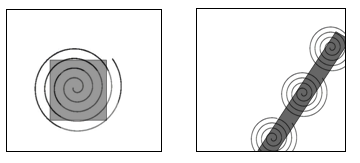
\includegraphics[width=8cm,height=2.2cm]{DSSR/block2.png}
\caption{DSSR covering block and strip pattern}
\label{fig:block2}
\end{figure}

Figure \ref{fig:block2} shows how DSS explores the failures residing in the block and strip patterns of a program. The coverage of block and strip pattern is shown in spiral form because first failure leads to second, second to third and so on till the end. In case the failure is positioned on the point pattern then the added values may not be effective because point pattern is only an arbitrary failure point in the whole input domain.

\subsection{Structure of the Dirt Spot Sweeping Random Strategy}

The DSSR strategy continuously tracks the number of failures during the execution of the test. This tracking is done in a very effective way with zero or minimum overhead to keep the overhead up to bare minimum~\cite{Leitner2009}. The test execution is started by R+ strategy and continues till a failure is found in the SUT after which the program copies the values leading to the failure as well as the surrounding values to the variable list of interesting values. 

\begin{figure}[ht]
\centering
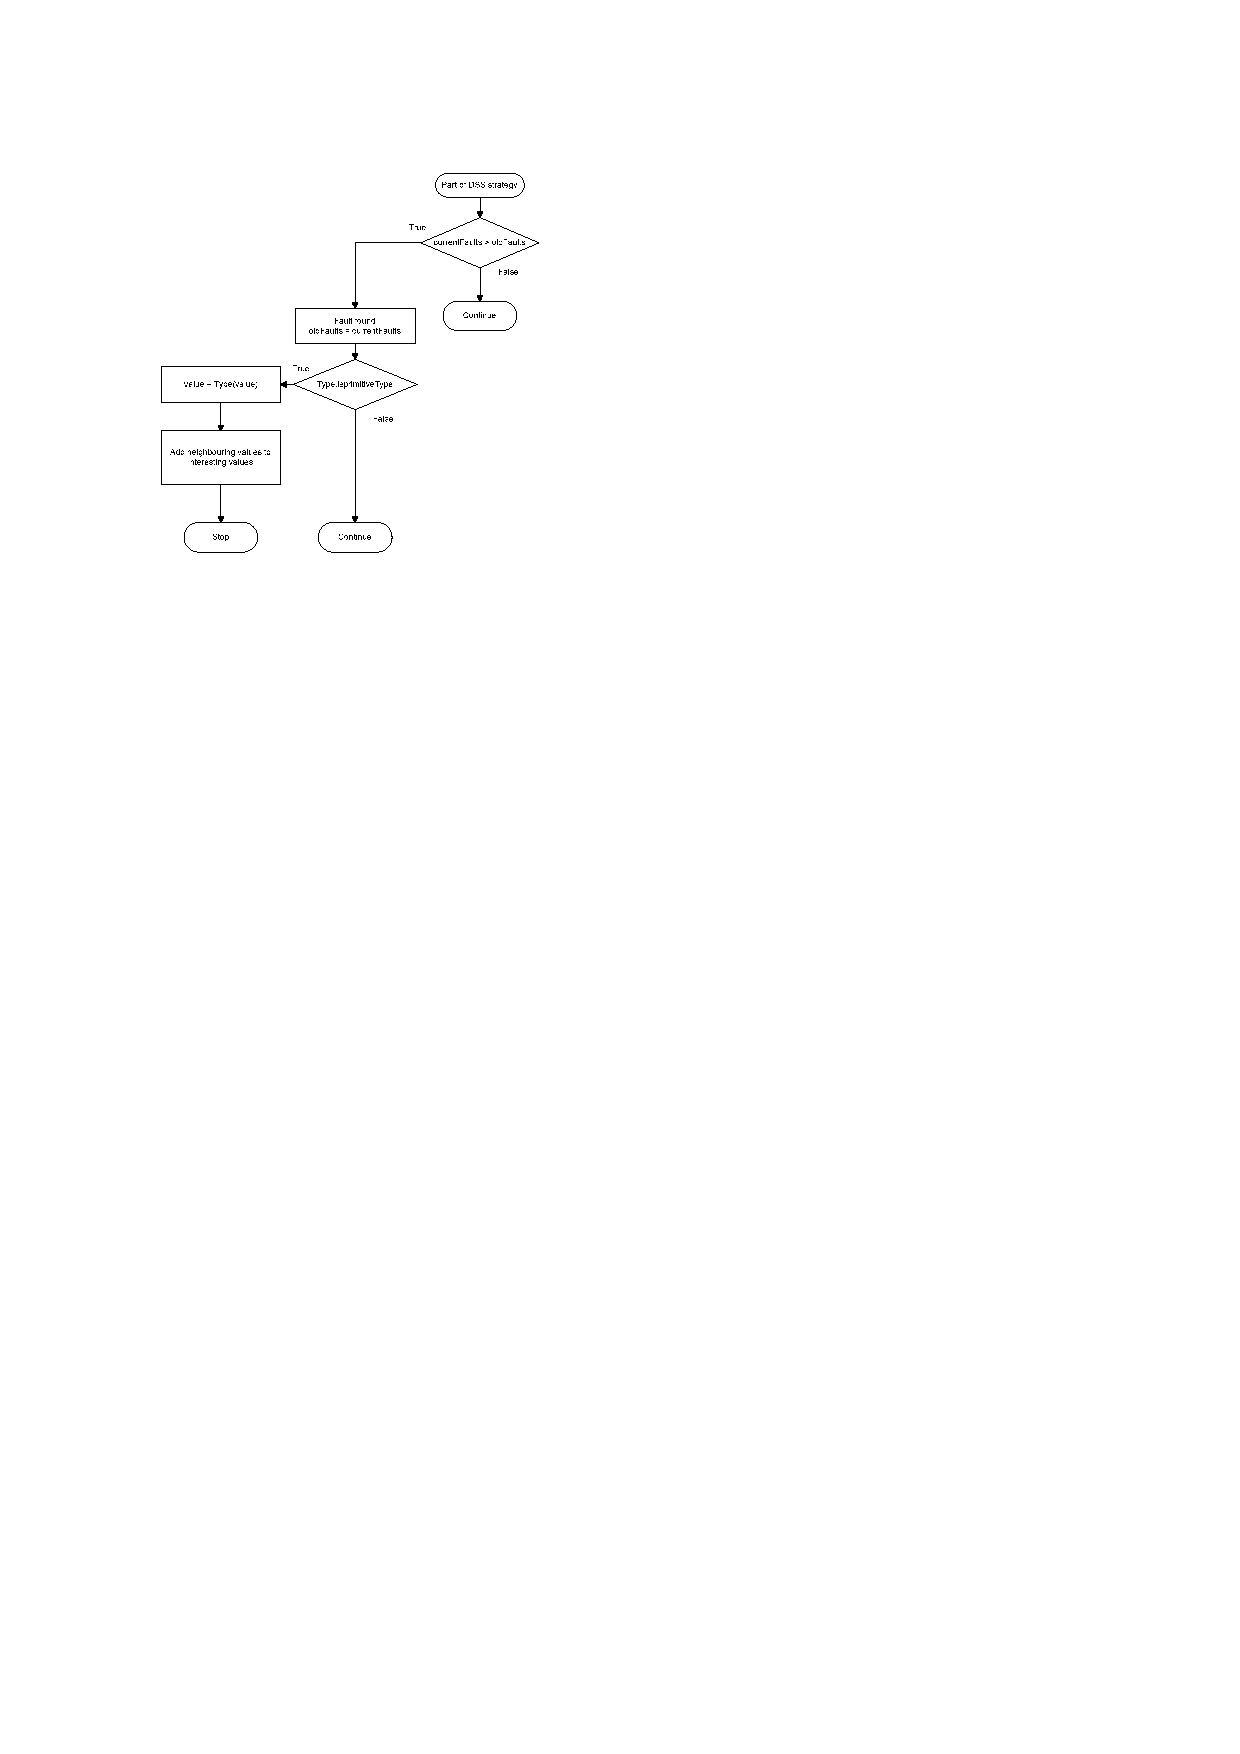
\includegraphics[width=10cm, height=12cm]{DSSR/flowchart1.pdf}
\caption{Working mechanism of DSSR Strategy}
\label{fig:Working_DSSS}
\end{figure}

The flowchart presented in Figure~\ref{fig:Working_DSSS} depicts that, when the failure finding value is of primitive type, the DSSR strategy identifies its type and add values only of that particular type to the list of interesting values. The resultant list of interesting values provide relevant test data for the remaining test session and the generated test cases are more targeted towards finding new failures around the existing failures in the given SUT.

Boundary and other special values that have a high tendency of finding faults in the SUT are added to the list of interesting values by random+ strategy prior to the start of test session where as in DSSR strategy the fault-finding and its surrounding values are added at runtime when a failure is found. 

Table \ref{table:addvalues2} presents the values are added to the list of interesting values when a failure is found. In the table the test value is represented by X where X can be int, double, float, long, byte, short, char and String. All values are converted to their respective types before adding them to the list of interesting values.

\begin{table}[ht]
%\scriptsize
\caption{Neighbouring values for primitive types and String} % title of Table
\smallskip
\centering % used for centering table
\begin{tabular}{| l | l |} % centered columns (4 columns)
\hline\hline %inserts double horizontal lines
Type & Values to be added\\ [0.5ex] % inserts table
%heading
\hline % inserts single horizontal line
\multirow{1}{*}{X is int, double, float, } & ~ X,  X+1, X+2, X-1, X-2 \\ % inserting body of the
\multirow{1}{*}{long, byte, short \& char} &  \\ 

\hline
\multirow{8}{*}{X is String} & ~ X\\ % inserting body of the table

& ~ X + ``  "\\ % inserting body of the table
& ~ ``  " + X \\ % inserting body of the table
& ~ X.toUpperCase() \\
& ~ X.toLowerCase() \\
& ~ X.trim() \\
& ~ X.substring(2) \\
& ~ X.substring(1, X.length()-1) \\[1ex]
\hline
\hline %inserts single line
\end{tabular}
\bigskip
\label{table:addvalues2} % is used to refer this table in the text
\end{table}





%%%%%%%%%%%%%%%%%%%%%%%%%%%%% EXPLANATION OF DSSR STRATEGY %%%%%%%%%%%%%%%%%%%%%%%%%%


\subsection{Explanation of DSSR strategy on a concrete example}
The DSSR strategy is explained through a simple program seeded with three faults. The first fault is a division by zero exception denoted by 1 while the second and third faults are failing assertion denoted by 2 and 3 in the given program below followed by description of how the strategy perform execution.

\begin{lstlisting}
/** 
* Calculate square of given number 
* and verify results. 
* The code contain 3 faults.
* @author (Mian and Manuel)
*/
public class Math1 {
 public void calc (int num1) {
  // Square num1 and store result. 
  int result1 = num1 * num1;
  int result2 = result1 / num1; // 1
  assert Math.sqrt(result1) == num1; // 2
  assert result1 >= num1; // 3
 } 
}
\end{lstlisting}

In the above code, one primitive variable of type \verb+int+ is used, therefore, the input domain for DSSR strategy is from \verb+-2,147,483,648 to 2,147,483,647+. The strategy further select values (\verb+0, Integer.MIN_VALUE+ \& \verb+Integer.MAX_VALUE+) as interesting values which are prioritised for selection as inputs. 
As the test starts, three faults are quickly discovered by DSSR strategy in the following order.

\indent \textbf{Fault 1:} The strategy select value \verb+0+ for variable \verb+num1+  in the first test case because \verb+0+ is available in the list of interesting values and therefore its priority is higher than other values. This will cause Java to generate division by zero exception (1).

\indent \textbf{Fault 2:} After discovering the first fault, the strategy adds it and its surrounding values to the list of interesting values i.e. \verb+0, 1, 2, 3 and -1, -2, -3+ in this case. In the second test case the strategy may pick \verb+-3+ as a test value which may lead to the second fault where assertion (2) fails because the square root of \verb+9+ is \verb+3+ instead of the input value -3.

\indent \textbf{Fault 3:} After a few tests the strategy may select \\ \verb+Integer.MAX_VALUE+ for variable \verb+num1+  from the list of interesting values leading to discovery of the 3rd fault because int variable \verb+result1+ will not be able to store the square of \\ \verb+Integer.MAX_VALUE+. Instead of the actual square value Java assigns a negative value (Java language rule) to variable result1 that will lead to the violation of the next assertion (3).

The above process explains that including the border, fault-finding and surrounding values to the list of interesting values in DSSR strategy lead to the available faults quickly and in fewer tests as compared to random and random+ strategy. R and R+ takes more number of tests and time to discover the second and third faults because in these strategies the search for new unique failures starts again randomly in spite of the fact that the remaining faults are very close to the first one.


%%%%%%%%%%%%%%%%%    IMPLEMENTATION OF DSSR STRATEGY   %%%%%%%%%%%%


\section{Implementation of the DSSR strategy}\label{sec:imp}

Implementation of the DSSR strategy is made in the YETI open-source automated random testing tool. YETI, coded in Java language, is capable of testing systems developed in procedural, functional and object-oriented languages. Its language-agnostic meta model enables it to test programs written in multiple languages including Java, C\#, JML and .Net. The core features of YETI include easy extensibility for future growth, high speed ( up to one million calls per minute on java code), real time logging, real time GUI support, capability to test programs with multiple strategies and auto generation of test report at the end of test session. For large-scale testing there is a cloud-enabled version of YETI, capable of executing parallel test sessions in Cloud~\cite{Oriol2010}. A number of hitherto faults have successfully been found by YETI in various production softwares~\cite{Oriol2011, Oriol2012}.

YETI can be divided into three decoupled main parts: the core infrastructure, language-specific bindings and strategies. The core infrastructure contains representation for routines, a group of types and a pool of specific type objects. The language specific bindings contain the code to make the call and process the results. The strategies define the procedure of selecting the modules (classes), the routines (methods) and generation of values for instances involved in the routines. By default, YETI uses the random strategy if no particular strategy is defined during test initialisation. It also enables the user to control the probability of using null values and the percentage of newly created objects for each test session. YETI provides an interactive Graphical User Interface (GUI) in which users can see the progress of the current test in real time. In addition to GUI, YETI also provides extensive logs of the test session for more in-depth analysis.

The DSSR strategy is an extension of YetiRandomPlusStrategy, an extended form of the YetiRandomStrategy. The class hierarchy is shown in Figure \ref{fig:hierarchyofDSSR}.

\begin{figure}[h]
\centering
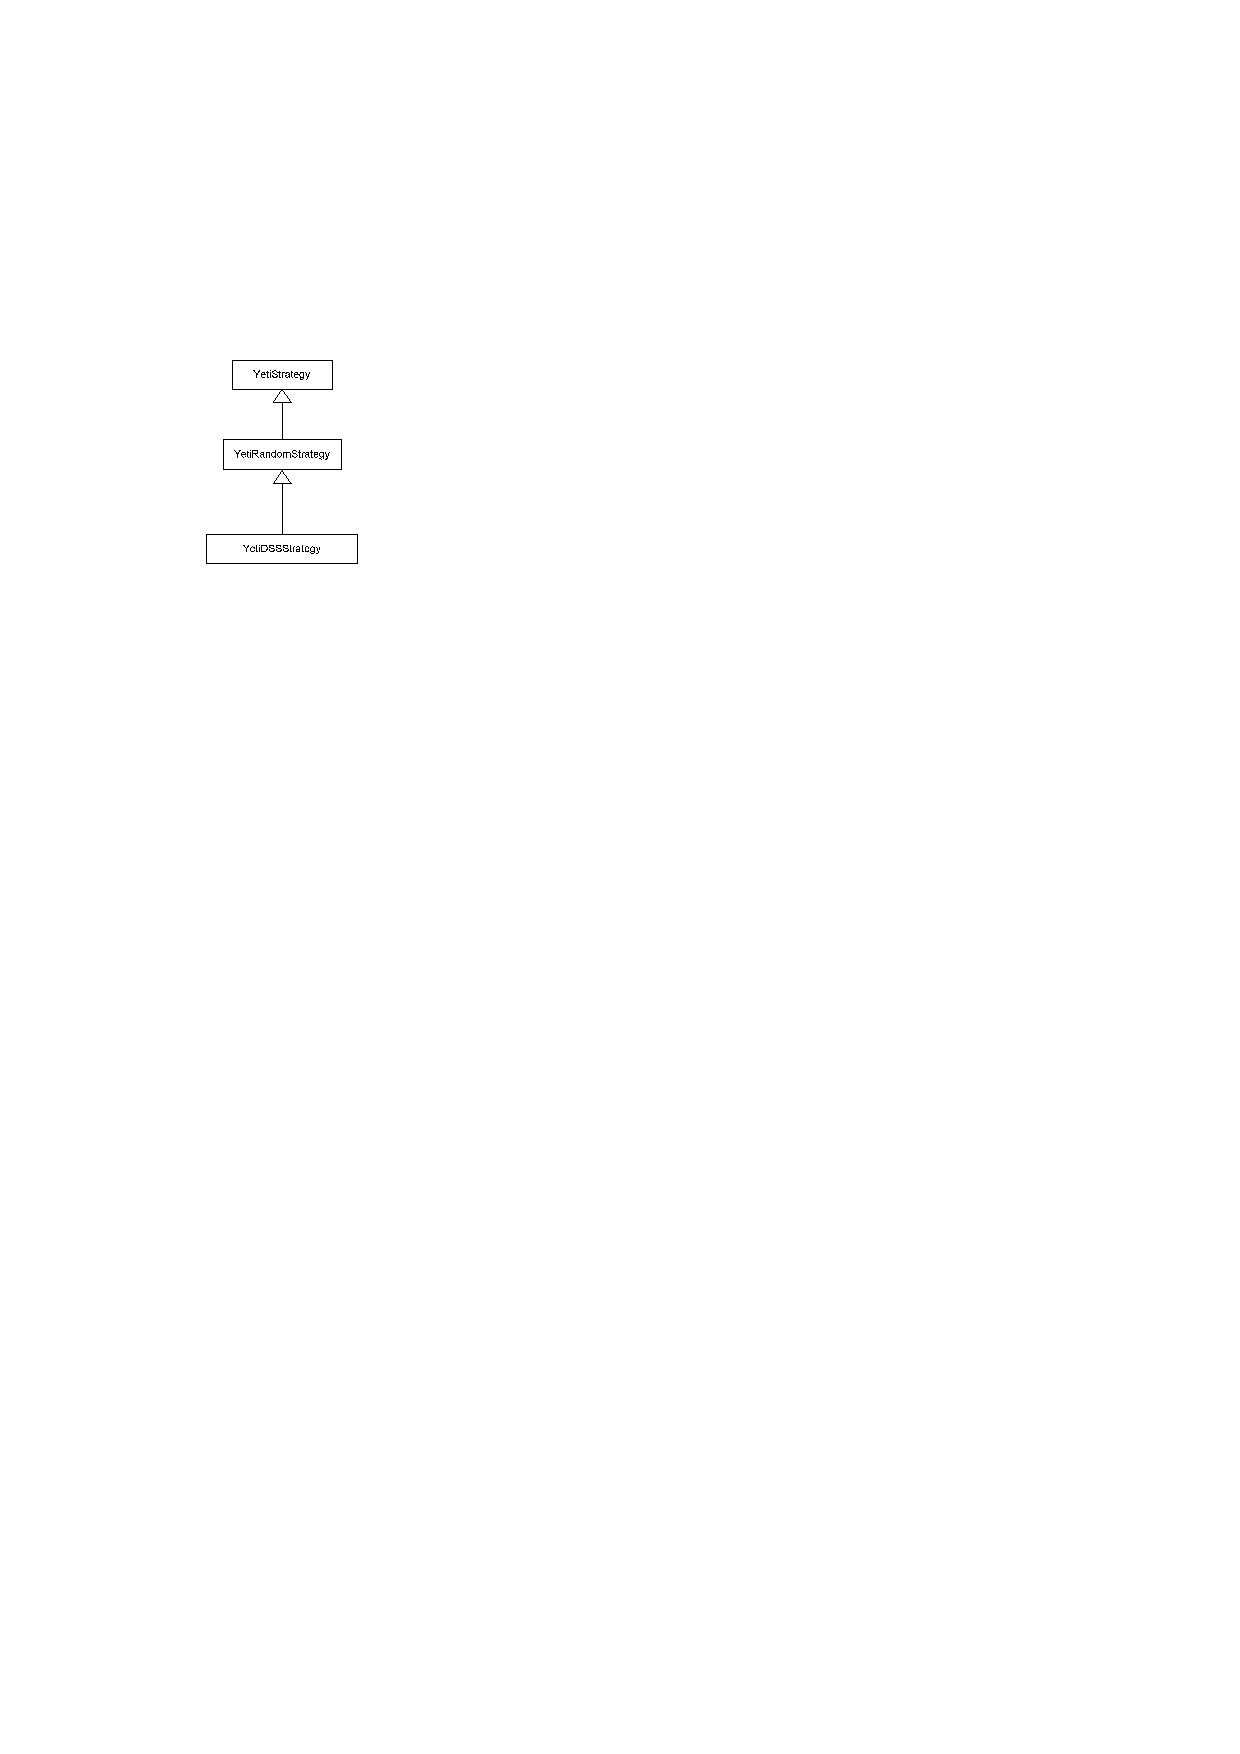
\includegraphics[width=4cm,height=5cm]{DSSR/hierarchy.pdf}
\caption{Class Hierarchy of DSSR in YETI}
\label{fig:hierarchyofDSSR}
\end{figure}





%%%%%%%%%%%%%%%%%    EVALUATION   %%%%%%%%%%%%%%%%%%%%


\section{Evaluation}\label{sec:eval}

The DSSR strategy is experimentally evaluated by comparing its performance with that of random and random+ strategy ~\cite{Leitner2007}. General factors such as system software and hardware, YETI specific factors like percentage of null values, percentage of newly created objects and interesting value injection probability have been kept constant in the experiments.

\subsection{Research questions}
For evaluating the DSSR strategy, the following research questions have been addressed in this study:
\begin{enumerate}
\item Is there an absolute best among R, R+ and DSSR strategies?
\item Are there classes for which any of the three strategies provide better results?
\item Can we pick the best default strategy between R, R+ and DSSR?
\end{enumerate}



\subsection{Experiments}

To evaluate the performance of DSSR we performed extensive testing of programs from the Qualitas Corpus~\cite{Tempero2010a}. The Qualitas Corpus is a curated collection of open source java projects built with the aim of helping empirical research on  software engineering. These projects have been collected in an organised form containing the source and binary forms. Version 20101126, which contains 106 open source java projects is used in the current evaluation. In our experiments we selected 60 random classes from 32 random projects. All the selected classes produced at least one fault and did not time out with maximum testing session of 10 minutes. Every class is tested thirty times by each strategy (R, R+, DSSR). Name, version and size of the projects to which the classes belong are given in table~\ref{table:projects} while test details of the classes is presented in table~\ref{table:Results}. Line of Code (LOC) tested per class and its total is shown in column 3 of table~\ref{table:Results}. 

Every class is evaluated through $10^5$ calls in each test session.\footnote{The total number of tests is thus $60\times 30\times 3 \times 10^5 = 540\times 10^6~tests$.} 
Because of the absence of the contracts and assertions in the code under test, Similar approach as used in previous studies ~\cite{Oriol2012} is followed using undeclared exceptions to compute unique failures.


\begin{table}[htp]
\caption{Name and versions of 32 Projects randomly selected from the Qualitas Corpus for the experiments}
\centering
\begin{tabular}{|r|l|r|r|}
\hline
S. No& 	Project Name	& 	Version		&	Size (MB)\\
\hline
1	&	apache-ant	&	1.8.1			&	59\\
2	&	antlr			&	3.2			&	13\\
3	&	aoi			&	2.8.1			&	35\\
4	&	argouml		&	0.30.2		&	112\\
5	&	artofillusion	&	281			&	5.4\\
6	&	aspectj		&	1.6.9			&	109.6\\
7	&	axion		&	1.0-M2		&	13.3\\
8	&	azureus		&	1			&	99.3\\
9	&	castor		&	1.3.1			&	63.2\\
10	&	cayenne		&	3.0.1			&	4.1\\
11	&	cobertura		&	1.9.4.1		&	26.5\\
12	&	colt			&	1.2.0			&	40\\
13	&	emma		&	2.0.5312		&	7.4\\
14	&	freecs		&	1.3.20100406	&	11.4\\
15	&	hibernate		&	3.6.0			&	733\\
16	&	hsqldb		&	2.0.0			&	53.9\\
17	&	itext			&	5.0.3			&	16.2\\
18	&	jasml		&	0.10			&	7.5 \\
19	&	jmoney		&	0.4.4			&	5.3\\
20	&	jruby			&	1.5.2			&	140.7\\
21	&	jsXe			&	04\_beta		&	19.9\\
22	&	quartz		&	1.8.3			&	20.4\\
23	&	sandmark		&	3.4			&	18.8\\
24	&	squirrel-sql	&	3.1.2			&	61.5\\
25	&	tapestry		&	5.1.0.5		&	69.2\\
26	&	tomcat		&	7.0.2			&	24.1\\
27	&	trove			&	2.1.0			&	18.2\\
28	&	velocity		&	1.6.4			&	27.1\\
29	&	weka		&	3.7.2			&	107\\
30	&	xalan		&	2.7.1			&	85.4\\
31	&	xerces		&	2.10.0		&	43.4\\
32	&	xmojo		&	5.0.0			&	15\\
\hline
\end{tabular}
\bigskip
\label{table:projects}
\end{table}



All tests are performed with a 64-bit Mac OS X Lion Version 10.7.4 running on 2 x 2.66 GHz 6-Core Intel Xeon processor with 6 GB (1333 MHz DDR3) of RAM. YETI runs on top of the Java\texttrademark  SE Runtime Environment [version 1.6.0\_35]. The machine took approximately 100 hours to process the experiments.


\subsection{Performance measurement criteria}
Various measures including the E-measure (expected number of failures detected), P-measure (probability of detecting at least one failure) and F-measure (number of test cases used to find the first fault) have been used by researchers to find the effectiveness of the random test strategy. The E-measure and P-measure have been heavily criticised~\cite{Chen2008} and are not considered effective measuring techniques while the F-measure has been often used by various researchers~\cite{Chen1996, Chen2004}. In our initial experiments the F-measure is used to evaluate the efficiency. However it was realised that this is not the right choice. In some experiments a strategy found the first fault quickly than the other but on completion of test session that very strategy found lower number of total faults than the rival strategy. The preference given to a strategy by F-measure because it finds the first fault quickly without giving due consideration to the total number of faults is not fair~\cite{Liu2012}.


  
The literature review revealed that the F-measure is used where testing stops after identification of the first fault and the system is given back to the developers to remove the fault. Currently automated testing tools test the whole system and print all discovered faults in one go therefore, F-measure is not the favourable choice. In our experiments, performance of the strategy is measured by the maximum number of faults detected in SUT by a particular number of test calls \cite{Pacheco2007a, Ciupa2007, Ciupa2008b}. This measurement is effective because it considers the performance of the strategy when all other factors are kept constant.

%%%%%%%%%%%%%%%%%    RESULTS   %%%%%%%%%%%%%%%%%%%%
\begin{figure*}[ht]
\centering
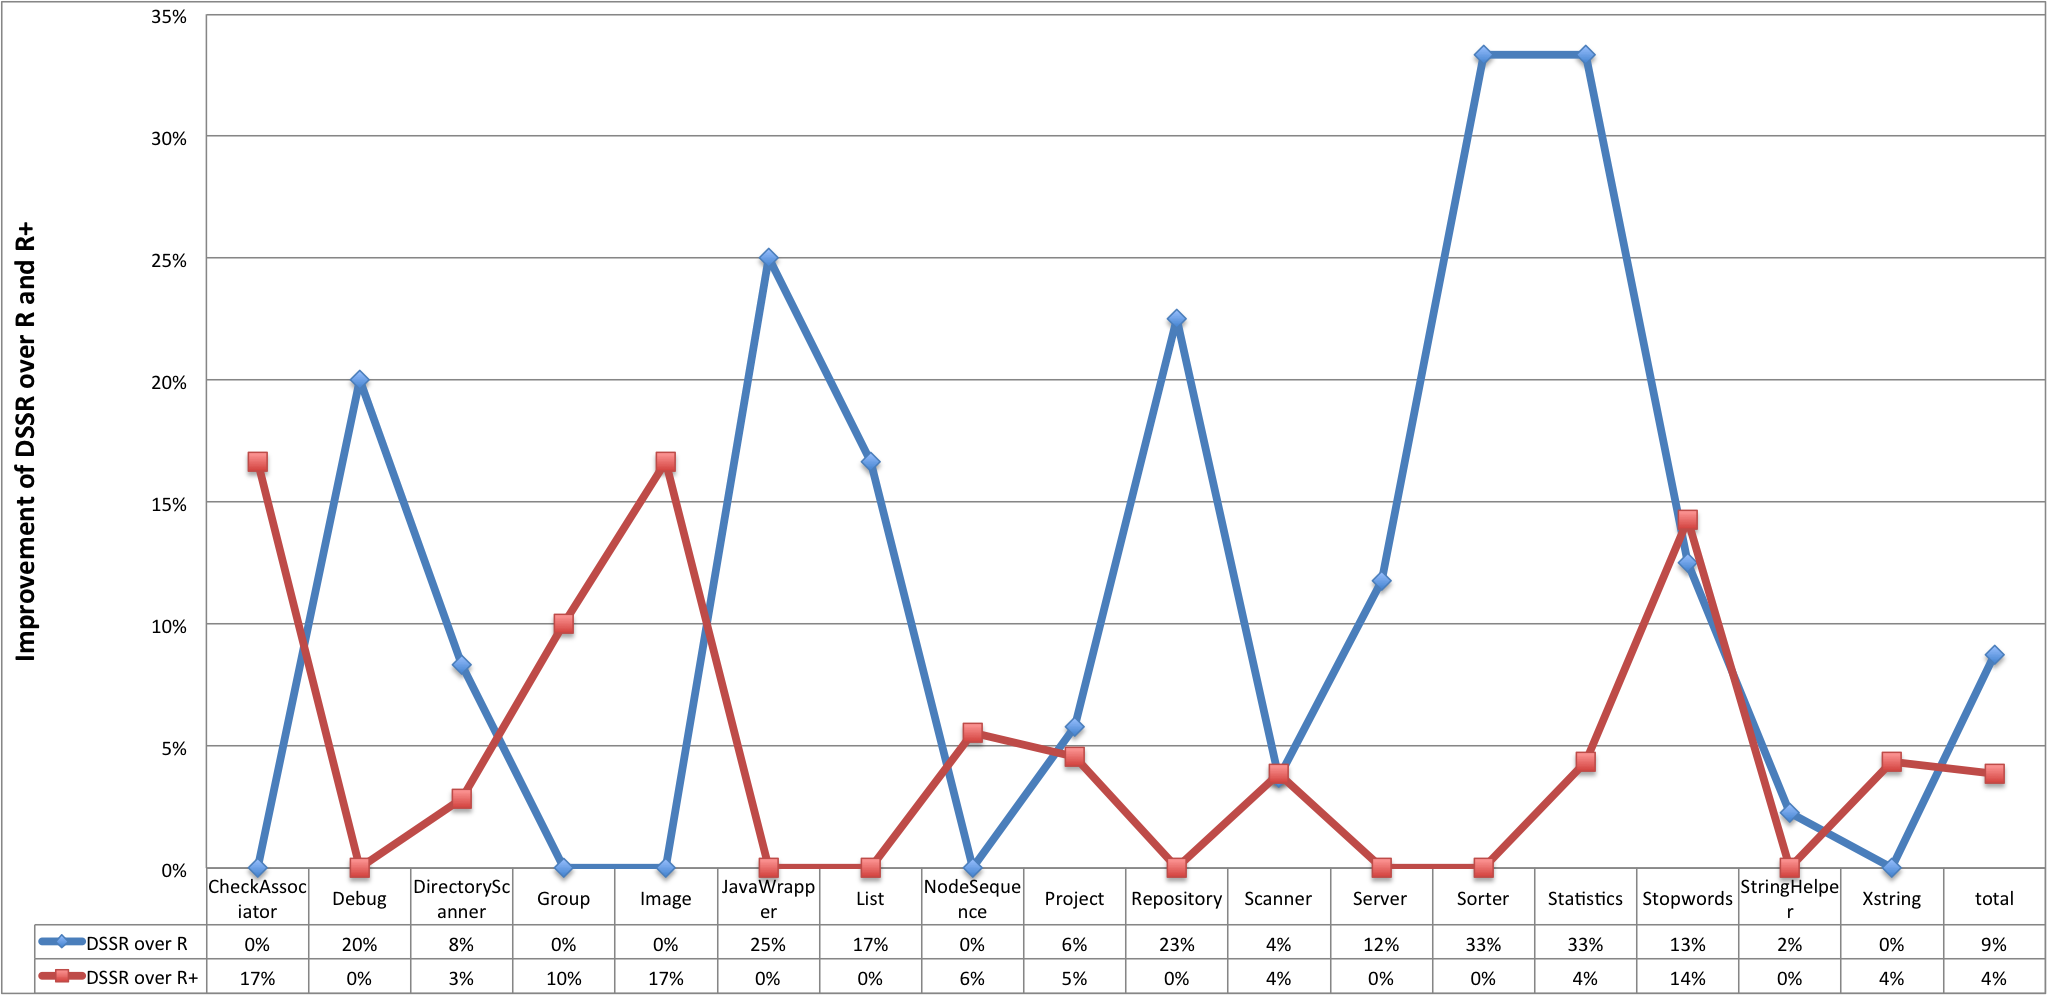
\includegraphics[width=14cm]{DSSR/DssrImprove.png}
\caption{Improvement of DSSR strategy over Random and Random+ strategy.}
\label{fig:LineChart}
\end{figure*}

%%%%%%%%%%%%%%%%%%%%%%%%%%%%%%%%%%%%%%%%%%%%



\begin{table*} [htp!]
  \scriptsize
 \caption{Experiments result presenting Serial Number (S.No), Class Name, Line of Code (LOC), mean, maximum and minimum number of faults and relative standard deviation for each Random (R), Random+ (R+) and Dirt Spot Sweeping Random (DSSR) strategies.}
	%\begin{minipage}[h]{\pagewidth}\centering
	\hspace{-2cm}
	\noindent\makebox[\textwidth]{
 	\begin{tabularx}{1 \textwidth}{r l r r r r r r r r r r r r r}
      %\aline

      \multirow{2}{*}{S. No}		& \multirow{2}{*}{Class Name}		& \multirow{2}{*}{LOC}	& \multicolumn{4}{c}{R}							&	\multicolumn{4}{c}{R+}							&	\multicolumn{4}{c}{DSSR}	\\
      %\cline{3-14} 
      						&						&			& Mean 	& Max	& Min 	& 	R-STD				& Mean 	& Max 	& Min 	&	 R-STD 			& Mean 		& Max 		& Min		& R-STD \\


1						& ActionTranslator			&709		& 96		&	96	&	96	& 	0					& 96		& 96 		& 96		& 		0			& 96			& 96			& 96			&	0\\     
2						& AjTypeImpl				&1180		& 80		&	83	&	79	& 	0.02					& 80		& 83 		& 79		& 		0.02			& 80			& 83			& 79			&	0.01\\      
\textbf{3}					& \textbf{Apriori}			&\textbf{292}	& \textbf{3}&	\textbf{4}	&\textbf{3}	& \textbf{0.10}			& \textbf{3}& \textbf{4} 		& \textbf{3}& \textbf{0.13}	& \textbf{3}	& \textbf{4}	& \textbf{3}	&\textbf{0.14}\\      
4						& BitSet					&575		& 9		&	9	&	9	& 	0					& 9		& 9 		& 9		& 		0			& 9			& 9			& 9			&	0\\       
5						& CatalogManager			&538		& 7		&	7	&	7	& 	0					& 7		& 7 		& 7		& 		0			& 7			& 7			& 7			&	0\\    
\textbf{6}					& \textbf{CheckAssociator}	&\textbf{351}	& \textbf{7}	&	\textbf{8}	&	\textbf{2}	& 	\textbf{0.16}					& \textbf{6}		& \textbf{9} 		& \textbf{2}		& 		\textbf{0.18}			& \textbf{7}			& \textbf{9}			& \textbf{6}			&	\textbf{0.73}\\    
\textbf{7}						& \textbf{Debug}					&\textbf{836}		& \textbf{4}		&	\textbf{6}	&	\textbf{4}	& 	\textbf{0.13}					& \textbf{5}		& \textbf{6} 		& \textbf{4}		& 		\textbf{0.12}			& \textbf{5}			& \textbf{8}			& \textbf{4}			&	\textbf{0.19}\\       
\textbf{8}						& \textbf{DirectoryScanner}			&\textbf{1714}		& \textbf{33}		&	\textbf{39}	&	\textbf{20}	& 	\textbf{0.10}					& \textbf{35}		& \textbf{38} 		& \textbf{31}		& 		\textbf{0.05}			& \textbf{36}			& \textbf{39}			& \textbf{32}			&	\textbf{0.04}\\      
9						& DiskIO					&220		& 4		&	4	&	4	& 	0					& 4		& 4 		& 4		& 		0			& 4			& 4			& 4			&	0\\      
10						& DOMParser				&92			& 7		&	7	&	3	& 	0.19					& 7		& 7 		& 3		& 		0.11			& 7			& 7			& 7			&	0\\      
11						& Entities					&328		& 3		&	3	&	3	& 	0					& 3		& 3 		& 3		& 		0			& 3			& 3			& 3			&	0\\      
12						& EntryDecoder			&675		& 8		&	9	&	7	& 	0.10					& 8		& 9 		& 7		& 		0.10			& 8			& 9			& 7			&	0.08\\   
13						& EntryComparator			&163		& 13		&	13	&	13	& 	0					& 13		& 13 		& 13		& 		0			& 13			& 13			& 13			&	0\\      
14						& Entry					&37			& 6		&	6	&	6	& 	0					& 6		& 6 		& 6		& 		0			& 6			& 6			& 6			&	0\\   
15						& Facade					&3301		& 3		&	3	&	3	& 	0					& 3		& 3 		& 3		& 		0			& 3			& 3			& 3			&	0\\   
16						& FileUtil					&83			& 1		&	1	&	1	& 	0					& 1		& 1 		& 1		& 		0			& 1			& 1			& 1			&	0\\      
17						& Font					&184		&12		&	12	&	11	& 	0.03					& 12		& 12 		& 11		& 		0.03			& 12			& 12			& 11			&	0.02\\        
18						& FPGrowth				&435		& 5		&	5	&	5	& 	0					& 5		&  5		& 5		& 		0			& 5			& 5			& 5			&	0	\\       
19						& Generator				&218		& 17		&	17	&	17	& 	0					& 17		& 17 		& 17		& 		0			& 17			& 17			& 17			&	0	\\      
\textbf{20}						& \textbf{Group}					&\textbf{88}			& \textbf{11}		&	\textbf{11}	&	\textbf{10}	& 	\textbf{0.02}					& \textbf{10}		& \textbf{4} 		& \textbf{11}		& 		\textbf{0.15}			& \textbf{11}			& \textbf{11}			& \textbf{11}			&	\textbf{0}	\\      
21						& HttpAuth				&221		& 2		&	2	&	2	& 	0					& 2		& 2 		& 2		& 		0			& 2			& 2			& 2			&	0	\\         
\textbf{22}						& \textbf{Image}					&\textbf{2146}		& \textbf{13}		&	\textbf{17}	&	\textbf{7}	& 	\textbf{0.15}					& \textbf{12}		& \textbf{14} 		& \textbf{4}	& 		\textbf{0.15}			& \textbf{14}			& \textbf{16}			& \textbf{11}			&	\textbf{0.07}\\        
23						& InstrumentTask			&71			& 2		&	2	&	1	& 	0.13					& 2		& 2 		& 1		& 		0.09			& 2			& 2			& 2			&	0	\\    
24						& IntStack					&313		& 4		&	4	&	4	& 	0					& 4		& 4 		& 4		& 		0			& 4			& 4			& 4			&	0	\\      
25						& ItemSet					&234		& 4		&	4	&	4	& 	0					& 4		& 4 		& 4		& 		0			& 4			& 4			& 4			&	0	\\       
26						& Itextpdf					&245		& 8		&	8	&	8	& 	0					& 8		&  8		& 8		& 		0			& 8			& 8			& 8			&	0\\      
\textbf{27}						& \textbf{JavaWrapper}				&\textbf{513}		&\textbf{3}		&	\textbf{2}	&	\textbf{2}	& 	\textbf{0.23}					& \textbf{4}		& \textbf{4} 		& \textbf{3}		& 		\textbf{0.06}			& \textbf{4}			& \textbf{4}			& \textbf{3}			&	\textbf{0.05}\\      
28						& JmxUtilities				&645		& 8		&	8	&	6	& 	0.07					& 8		& 8 		& 7		& 		0.04			& 8			& 8			& 7			&	0.04\\      
\textbf{29}						& \textbf{List}					&\textbf{1718}		& \textbf{5}		&	\textbf{6}	&	\textbf{4}	& 	\textbf{0.11}					& \textbf{6}		& \textbf{6} 		& \textbf{4}		& 		\textbf{0.10}			&\textbf{6}			& \textbf{6}			& \textbf{5}			&	\textbf{0.09}\\      
30						& NameEntry				&172		& 4		&	4	&	4	& 	0					& 4		& 4 		& 4		& 		0			& 4			& 4			& 4			&	0	\\  
\textbf{31}						& \textbf{NodeSequence}			&\textbf{68}			& \textbf{38}		&	\textbf{46}	&	\textbf{30}	& 	\textbf{0.10}					& \textbf{36}		& \textbf{45} 		& \textbf{30}		& 		\textbf{0.12}			& \textbf{38}			& \textbf{45}			& \textbf{30}			&	\textbf{0.08}	\\     
32						& NodeSet				&208		& 28		&	29	&	26	& 	0.03					& 28		& 29 		& 26		& 		0.04			& 28			& 29			& 26			&	0.03	\\  
33						& PersistentBag			&571		& 68		&	68	&	68	& 	0					& 68		&  68		& 68		& 		0			& 68			& 68			& 68			&	0	\\         
34						& PersistentList				&602		& 65		&	65	&	65	& 	0					& 65		&  65		& 65		& 		0			& 65			& 65			& 65			&	0	\\    
35						& PersistentSet				&162		& 36		&	36	&	36	& 	0					& 36		&  36		& 36		& 		0			& 36			& 36			& 36 			&	0	\\        
\textbf{36}						& \textbf{Project}					&\textbf{470}		& \textbf{65}		&	\textbf{71}	&	\textbf{60}	& 	\textbf{0.04}					& \textbf{66}		&  \textbf{78}		& \textbf{62}		& 		\textbf{0.04}			& \textbf{69}			& \textbf{78}			& \textbf{64}			&	\textbf{0.05}	\\        
\textbf{37}						& \textbf{Repository}				&\textbf{63}			& \textbf{31}		&	\textbf{31}	&	\textbf{31}	& 	\textbf{0}					& \textbf{40}		&  \textbf{40}		& \textbf{40}		& 		\textbf{0}			& \textbf{40}			& \textbf{40}			& \textbf{40}			&	\textbf{0}	\\         
38						& Routine					&1069		& 7		&	7	&	7	& 	0					& 7		&  7		& 7		& 		0			& 7			& 7			& 7			&	0	\\
39						& RubyBigDecimal			&1564		& 4 		&	4	&	4	& 	0					& 4		& 4 		& 4		& 		0			& 4			& 4			& 4			&	0\\      
40						& Scanner				&94			& 3		&	5	&	2	& 	0.20					& 3		& 5 		& 2		& 		0.27			& 3			& 5			& 2			&	0.25\\      
\textbf{41}						& \textbf{Scene}					&\textbf{1603}		& \textbf{26}		&	\textbf{27}	&	\textbf{26}	& 	\textbf{0.02}					& \textbf{26}		& \textbf{27} 		& \textbf{26}		& 		\textbf{0.02}			& \textbf{27}			& \textbf{27}			& \textbf{26}			&	\textbf{0.01}\\      
42						& SelectionManager			&431		& 3		&	3	&	3	& 	0					& 3		& 3 		& 3		& 		0			& 3			& 3			& 3			&	0\\      
\textbf{43}						& \textbf{Server}					&\textbf{279}		&\textbf{15}		&	\textbf{21}	&	\textbf{11}	& 	\textbf{0.20}					& \textbf{17}		& \textbf{21} 		& \textbf{12}		& 		\textbf{0.16}			& \textbf{17}			& \textbf{21}			& \textbf{12}			&	\textbf{0.14}\\      
\textbf{44}						& \textbf{Sorter}					&\textbf{47}			& \textbf{2}		&	\textbf{2}	&	\textbf{1}	& 	\textbf{0.09}					& \textbf{3}		& \textbf{3} 		& \textbf{2}		& 		\textbf{0.06}			&\textbf{3}			& \textbf{3}			& \textbf{3}			&	\textbf{0}\\      
45						& Sorting					&762		& 3		&	3	&	3	& 	0					& 3		& 3 		& 3		& 		0			& 3			& 3			& 3			&	0\\      
\textbf{46}						& \textbf{Statistics}				&\textbf{491}		& \textbf{16}		&	\textbf{17}	&	\textbf{12}	&	\textbf{0.08}					& \textbf{23}		& \textbf{25} 		& \textbf{22}		& 		\textbf{0.03}			& \textbf{24}			& \textbf{25}			& \textbf{22}			&	\textbf{0.04}\\      
47						& Status					&32			& 53		&	53	&	53	& 	0					& 53		& 53 		& 53		& 		0			& 53			& 53			& 53			&	0\\      
\textbf{48}						& \textbf{Stopwords}				&\textbf{332}		& \textbf{7}		&	\textbf{8}	&	\textbf{7}	& 	\textbf{0.03}					& \textbf{7}		&  \textbf{8}		& \textbf{6}		& 		\textbf{0.08}			& \textbf{8}			& \textbf{8}			& \textbf{7}			&	\textbf{0.06}\\      
\textbf{49}						& \textbf{StringHelper}				&\textbf{178}		& \textbf{43}	 	& 	\textbf{45}	&	\textbf{40}	& 	\textbf{0.02}					& \textbf{44}		&  \textbf{46}		& \textbf{42}		& 		\textbf{0.02}			& \textbf{44}			& \textbf{45}			& \textbf{42}			&	\textbf{0.02}\\      
50						& StringUtils				&119		& 19 		&	19	&	19	& 	0					& 19		& 19 		& 19		& 		0			& 19			& 19			& 19			&	0\\      
51						& TouchCollector			&222		& 3		&	3	&	3	& 	0					& 3		&  3		& 3		& 		0			& 3			& 3			& 3			&	0\\      
52						& Trie					&460		& 21		&	22	&	21	& 	0.02					& 21		&  22		& 21		& 		0.01			& 21			& 22			& 21			&	0.01\\      
53						& URI					&3970		& 5 		&	5	&	5	& 	0					& 5		&  5		& 5		& 		0			& 5			& 5			& 5			&	0\\      
54						& WebMacro				&311		& 5		&	5	&	5	& 	0					& 5		&  6		& 5		& 		0.14			& 5			& 7			& 5			&	0.28\\      
55						& XMLAttributesImpl			&277		& 8		&	8	&	8	& 	0					& 8		&  8		& 8		& 		0			& 8			& 8			& 8			&	0\\      
56						& XMLChar				&1031		& 13		&	13	&	13	& 	0					& 13		&  13		& 13		& 		0			& 13			& 13			& 13			&	0\\      
57						& XMLEntityManger			&763		& 17		&	18	&	17	& 	0.01					& 17		&  17		& 16		& 		0.01			& 17			& 17			& 17			&	0\\      
58						& XMLEntityScanner			&445		& 12		&	12	&	12	& 	0					& 12		&  12		& 12		& 		0			& 12			& 12			& 12			&	0\\      
59						& XObject					&318		& 19		&	19	&	19	& 	0					& 19		&  19		& 19		& 		0			& 19			& 19			& 19			&	0\\      
\textbf{60}						& \textbf{XString}					&\textbf{546}		& \textbf{23}		&	\textbf{24}	&	\textbf{21}	& 	\textbf{0.04}					& \textbf{23}		&  \textbf{24}		& \textbf{23}		& 		\textbf{0.02}			& \textbf{24}			& \textbf{24}			& \textbf{23}			&	\textbf{0.02}\\      

    						\multicolumn{2}{c}{\textbf{Total}}	&35,785	&1040	&	1075	&    973	&	2.42				& 1061	&1106	&1009	&		2.35		& 1075		& 1118		& 1032		& 	1.82\\
   %\hline
     \end{tabularx} }
 	%\end{minipage}
    \bigskip
    \label{table:Results}
\end{table*}

\section{Results}\label{sec:res}
Results of the experiments including class name, Line of Code (LOC), mean value, maximum and minimum number of unique failures and relative standard deviation for each of the 60 classes tested using R, R+ and DSSR strategy are presented in Table~\ref{table:Results}. Each strategy found an equal number of faults in 31 classes while in the remaining 29 classes the three strategies performed differently from one another. The total of mean values of unique failures in DSSR (1075) is higher than for R (1040) or R+ (1061) strategies. 
%Results given in Table~\ref{table:ttest} can be split into three different categories as shown in Table~\ref{table:categories}. 
DSSR also finds a higher number of maximum unique failures (1118) than both R (1075), and R+ (1106). DSSR strategy finds 43 and 12 more unique faults compared to R and R+ respectively. The minimum number of unique faults found by DSSR (1032) is also higher than for R (973) and R+ (1009) which attributes to higher efficiency of DSSR strategy over R and R+ strategies. 

% How to write relative standard deviation.
% Eventually, the standard deviations are all of the order of magnitude of .1\% for all strategies.

\subsection{Is there an absolute best among R, R+ and DSSR strategies?}
Based on our findings DSSR is at least as good as R and R+ in almost all cases, it is also significantly better than both R and R+ in 12\% of the classes. Figure~\ref{fig:LineChart} presents the average improvements of DSSR strategy over R and R+ strategy over the 17 classes for which there is a significant difference between DSSR and R or R+. The blue line with diamond symbol shows performance of DSSR over R and the red line with square symbols depicts the improvement of DSSR over R+ strategy. The classes where blue line with diamond symbols show the improvement of DSSR over R and red line with square symbols show the improvement of DSSR over R+. 

The improvement of DSSR over R and R+ strategy is calculated by applying the formula (1) and (2) respectively.

\begin{equation} \frac{Averagefaults_{(DSSR)} - Averagefaults_{(R)}}{Averagefaults_{(R)}} * 100  \end{equation}

\begin{equation} \frac{Averagefaults_{(DSSR)} - Averagefaults_{(R+)}}{Averagefaults_{(R+)}}  * 100 \end{equation}

The findings show that DSSR strategy perform up to 33\% better than R and up to 17\% better than R+ strategy. In some cases DSSR perform equally well with R and R+ but in no case DSSR performed lower than R and R+. Based on the results it can be stated that DSSR strategy is a better choice than R and R+ strategy. 

\begin{table*}[htp]
\small
\caption{T-test results of the classes}
\smallskip
\centering
\begin{tabular}{rlrrrl}
\hline
 \multirow{2}{*} {S. No}	& \multirow{2}{*}{Class Name}	&  \multicolumn{3}{c}{T-test Results} & \multirow{2}{*}{Interpretation} \\

		&					& 	DSSR, R			& DSSR, R+	&  R, R+ 		& 		\\
\hline
1		&	AjTypeImpl		&	1 				& 1 			& 1			& 		\\	
2		&	Apriori			&	\textbf{0.03}	 	& 0.49		& 0.16		&		\\	
3		&	CheckAssociator	&	\textbf{0.04}	 	& \textbf{0.05}	& 0.44		& DSSR better		\\	
4		&	Debug			&	\textbf{0.03}	 	& 0.14		& 0.56		&		\\	
5		&	DirectoryScanner	&	\textbf{0.04}	 	& \textbf{0.01}	& 0.43		& DSSR better		\\
6		&	DomParser		&	\textbf{0.05}	 	& 0.23		& 0.13		&				\\
7		&	EntityDecoder		&	\textbf{0.04}	 	& 0.28		& 0.3			&		\\			
8		&	Font				&	0.18	 			& 0.18		& 1			&		\\
9		&	Group			&	0.33	 			& \textbf{0.03}	& \textbf{0.04}	& DSSR = R \textgreater R+	\\
10		&	Image			&	\textbf{0.03}		& \textbf{0.01}	& 0.61		& DSSR better \\		
11		&	InstrumentTask		&	0.16				& 0.33		& 0.57		& \\
12		&	JavaWrapper		&	\textbf{0.001}		& 0.57		& 0.004		& DSSR = R+ \textgreater R \\
13		& 	JmxUtilities		&	0.13				& 0.71		& 0.08		&	\\
14		&	List				& 	\textbf{0.01}		&0.25		&\textbf{0}		& DSSR = R+ \textgreater R \\
15		&	NodeSequence	&	0.97				&\textbf{0.04}	&\textbf{0.06}	& DSSR = R \textgreater R+ \\
16		&	NodeSet			&	\textbf{0.03}		&0.42		&0.26		& 	\\
17		&	Project			&	\textbf{0.001}		&0.57		&\textbf{0.004}	& DSSR better \\		
18		&	Repository		&	\textbf{0}			&1			&\textbf{0}		& DSSR = R+ \textgreater R \\
19		&	Scanner			&	1				&\textbf{0.03}	&\textbf{0.01}	& DSSR better \\
20		&	Scene			&	\textbf{0}			&\textbf{0}		& 1			& DSSR better \\
21		&	Server			&	\textbf{0.03}		& 0.88		&\textbf{0.03} 	& DSSR = R+ \textgreater R \\
22		&	Sorter			& 	\textbf{0}			& 0.33		&\textbf{0}		& DSSR = R+ \textgreater R \\
23		&	Statistics			&	\textbf{0}			& 0.43		&\textbf{0}		& DSSR = R+ \textgreater R\\
24		&	Stopwords		&	\textbf{0}			& 0.23		&\textbf{0}		& DSSR = R+ \textgreater R \\
25		&	StringHelper		&	\textbf{0.03}		& 0.44		&0.44		& DSSR = R+ \textgreater R\\
26		& 	Trie				&	0.1				& 0.33		&0.47		& DSSR better \\
27		&	WebMacro		&	0.33				& 1			&0.16		& \\
28		&	XMLEntityManager	&	0.33				& 0.33		&0.16		& \\
29 		&	XString			&	0.14				&\textbf{0.03}	&0.86		& \\


\end{tabular}
\bigskip
\label{table:ttest}
\end{table*}

\subsection{Are there classes for which any of the three strategies provide better results?}


T-tests applied to the data given in Table~\ref{table:ttest} show that DSSR is significantly better in 7 classes from R and R+ strategy, in 8 classes DSSR performed similarly to R+  but significantly higher than R, and in 2 classes DSSR performed similarly to R but significantly higher than R+. There is no case R and R+ strategy performed significantly better than DSSR strategy. Expressed in percentage: 72\%  of the classes do not show significantly different behaviours whereas in 28\% of hte classes, the DSSR strategy performs significantly better than at least one of R and R+. It is interesting to note that in no single case R and R+ strategies performed better than DSSR strategy. We attribute this to DSSR possessing the qualities of R and R+ whereas containing the spot sweeping feature.


%Results of the 60 classes tested in the study are divided in to 11 different categories as presented in ~\ref{table:categories}. 
\begin{comment}
\begin{table}[h]
\caption{Results of the 60 classes are divided into 11 categories}
\centering
\begin{tabular}{|r|l|r|}
\hline
S. No	& 	Category			& 	Result\\
\hline
1		&	DSSR > R			&	12 \\	
2		&	DSSR > R+		&	10 \\	
3		&	DSSR = R			&	5 \\	
4		&	DSSR = R+		&	7 \\	
5		&	R+ > R 			&	10 \\	
6		&	R+ < R			&	5 \\	
7		&	R+ = R			&	2 \\	
8		&	R > R+			&	4 \\
9		&	DSSR < R			&	0 \\	
10		&	DSSR < R+		&	0 \\
11		&	DSSR = R = R+	&	43 \\			
\hline
\end{tabular}
\bigskip
\label{table:categories}
\end{table}

% pie chart is removed because the length of the paper is exceeding 10 pages and also it don't make much sense i believe.
%\begin{figure}[h]
%\centering
%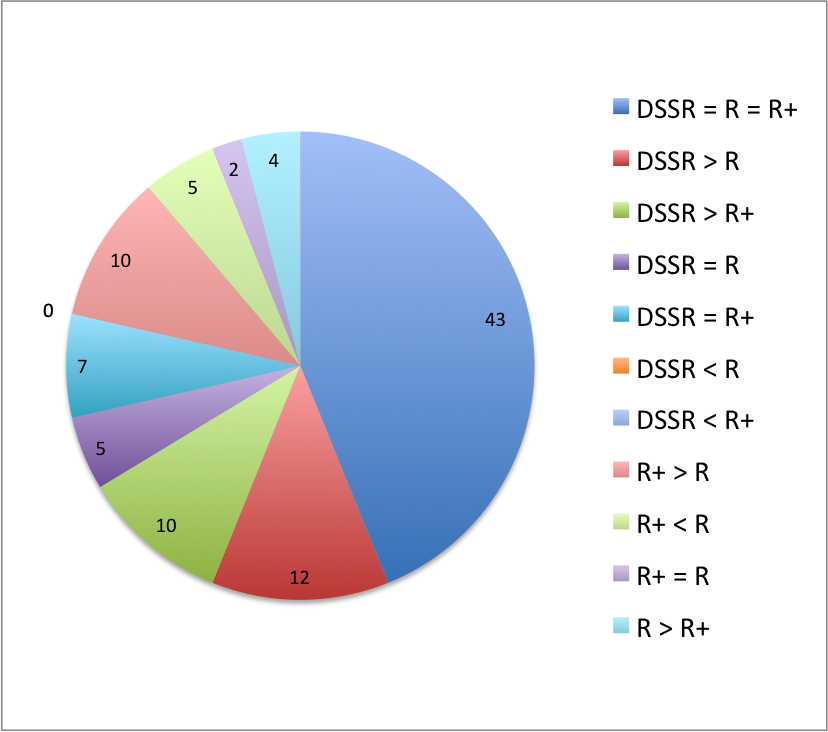
\includegraphics[width=8cm,height=7cm]{pie5.png}
%\caption{Division of result in to categories}
%\label{fig:pie}
%\end{figure}






The first category contain 12 classes where DSSR strategy performs better than R. 
The second category contain 10 classes where DSSR strategy performs better than R+. 
The third category contain 5 classes where DSSR strategy and R performs equally well.
The fourth category contain 7 classes where DSSR and R+ performs equally well. 
The fifth category contain 10 classes where R+ performs better than R.
The sixth category contain 5 classes where R performs better than R+.
The seventh category contain 2 classes where R and R+ performs equally well.
The eighth category contain 4 classes where R performs better than R+.
Category 9 and 10 shows that neither R nor R+ performed better than DSSR strategy.
The last category shows each strategy performing equally well for 43 classes. Expressing in percentage, 72\% classes do not show different behaviours whereas in 28\% of classes, the DSSR strategy performs better than R and R+ strategy. It is interesting to note that in no single case R and R+ strategies performed better than DSSR strategy. This is attributed to the fact that DSSR strategy possess the qualities of R and R+ and has the additional advantage of spot sweeping.

\end{comment}

\subsection{Can we pick the best default strategy between R, R+ and DSSR?}

Analysis of the experimental data reveal that DSSR strategy has an edge over R and R+. This is because of the additional feature of Spot Sweeping in DSSR strategy.

In spite of the better performance of DSSR strategy compared to R and R+ strategies the present study does not provide ample evidence to pick it as the best default strategy because of the overhead induced by this strategy (see next section). Further study might give conclusive evidence. 




%%%%%%%%%%%%%%%%%    DISCUSSION   %%%%%%%%%%%%%%%%%%%%

\section{Discussion}\label{sec:discussion3}
In this section we discuss various factors such as the time taken, effect of test duration, number of tests, number of faults in the different strategies and the effect of finding first fault in the DSSR strategy.
\textbf{Time taken to execute an equal number of test cases:}
The DSSR strategy takes slightly more time (up to 5\%) than both pure random and random plus which may be due to maintaining sets of interesting values during the execution. We do not believe that the overhead can be reduced. 

\textbf{Effect of test duration and number of tests on the results:}
All three techniques have the same potential for finding failures. If testing is continued for a long duration then all three strategies will find the same number of unique failures and the results will converge. We suspect however that some of the unique failures will take an extremely long time to be found by using random or random+ only. Further experiments should confirm this point.


\textbf{Effect of number of faults on results:} 
We found that the DSSR strategy performs better when the number of faults is higher in the code. The reason seems to be that when there are more faults, their domains are more connected and DSSR strategy works better. Further studies might use historical data to pick the best strategy.

\textbf{Dependence of DSSR strategy to find the first unique failure early enough:}
During the experiments we noticed that if a unique failure is not found  quickly enough, there is no value added to the list of interesting values and then the test becomes equivalent to random+ testing. This means that better ways of populating failure-inducing values are needed for sufficient leverage to DSSR strategy. As an example, the following piece of code would be unlikely to fail under the current setting:

\begin{lstlisting}
public void test(float value){
 if(value == 34.4445)   10/0;
}
\end{lstlisting}

In this case, we could add constant literals from the SUT to the list of interesting values in a dynamic fashion. These literals can be obtained from the constant pool in the class files of the SUT.

In the example above the value 34.4445 and its surrounding values would  be added to the list of interesting values before the test starts and the DSSR strategy would find the unique failure right away.

\textbf{DSSR strategy and coverage:} Random strategies typically achieve high level of coverage~\cite{Oriol2010}. It might also be interesting to compare R, R+ and DSSR with respect to the achieved coverage or even to use a DSSR variant that adds a new interesting value and its neighbours when a new branch is reached.


\textbf{Threats to validity:} As usual with such empirical studies, the present work might suffer from a non-representative selection of classes.
The selection in the current study is however made through random process and objective criteria, therefore, it seems likely that it would be representative.

The parameters of the study might also have prompted incorrect results. But this is unlikely due to previous results on random testing~\cite{Oriol2012}.



%%%%%%%%%%%%%%%%%    RW   %%%%%%%%%%%%%%%%%%%%

\section{Related Work}\label{sec:rw}

Random testing is a popular technique with simple algorithm but proven to find subtle faults in complex programs and Java libraries~\cite{Pacheco2005, Csallner2004, Claessen2000}. Its simplicity, ease of implementation and efficiency in generating test cases make it the best choice for test automation~\cite{hamlet1994}. Some of the well known automated tools based on random strategy includes Jartege~\cite{Oriat2004}, Eclat~\cite{Pacheco2005}, JCrasher~\cite{Csallner2004}, AutoTest \cite{Ciupa2007, Ciupa2008a} and YETI~\cite{Oriol2010, Oriol2012}.

In pursuit of better test results and lower overhead, many variations of random strategy have been proposed~\cite{Chen2010, Chen2005, Chan2002, Chen2004a, Chen2003}. Adaptive random testing (ART), Quasi-random testing (QRT) and Restricted Random testing (RRT) achieved better results by selecting test inputs randomly but evenly spread across the input domain. Mirror ART and ART through dynamic partitioning increased the performance by reducing the overhead of ART. The main reason behind better performance of the strategies is that even spread of test input increases the chance of exploring the fault patterns present in the input domain.

A more recent research study \cite{Yoo2012} stresses on the effectiveness of data regeneration in close vicinity of the existing test data. Their findings showed up to two orders of magnitude more efficient test data generation than the existing techniques. Two major limitations of their study are the requirement of existing test cases to regenerate new test cases, and increased overhead due to ``meta heuristics search'' based on hill climbing algorithm to regenerate new data. In DSSR no pre-existing test cases are required because it utilises the border values from R+ and regenerate the data very cheaply in a dynamic fashion different for each class under test without any prior test data and with comparatively lower overhead. 
  
The random+ (R+) strategy is an extension of the random strategy in which interesting values, beside pure random values, are added to the list of test inputs~\cite{Leitner2007}. These interesting values includes border values which have high tendency of finding faults in the given SUT~\cite{Beizer1990}. Results obtained with R+ strategy show significant improvement over random strategy~\cite{Leitner2007}. DSSR strategy is an extension of R+ strategy which starts testing as R+ until a fault is found then it switches to spot sweeping.

%It is interesting that numerous efforts have been made to discover the fault patterns~\cite{Chen2010, Chen2005, Chan2002, Chen2004a, Chen2003}, etc. but in our knowledge, none has been published on covering/sweeping all the faults lying in a specific pattern once it has been discovered.


A common practice to evaluate performance of an extended strategy is to compare the results obtained by applying the new and existing strategy to identical programs~\cite{Gutjahr1999, Duran1984, hamlet1990}. Arcuri et al. \cite{Arcuri2012}, stress on the use of random testing as a baseline for comparison with other test strategies. We followed the procedure and evaluated DSSR strategy against R and R+ strategies under identical conditions.

In our experiments we selected projects from the Qualitas Corpus~\cite{Tempero2010} which is a collection of open source java programs maintained for independent empirical research. The projects in Qualitas Corpus are carefully selected that spans across the whole set of java applications~\cite{Oriol2012, Tempero2010a, Tempero2008}.


%%%%%%%%%%%%%%%%%    CONCLUSIONS   %%%%%%%%%%%%%%%%%%%%


\section{Conclusions}\label{sec:conc}
The main goal of the present study was to develop a new random strategy which could find more faults in lower number of test cases. We developed a new strategy named. ``DSSR strategy'' as an extension of R+, based on the assumption that in a significant number of classes, failure domains are contiguous or located closely. The DSS strategy, a strategy which adds neighbouring values of the failure finding value to a list of interesting values, was implemented in the random testing tool YETI to test 60 classes, 30 times each, from Qualitas Corpus with each of the 3 strategies R, R+ and DSSR. The newly developed DSSR strategy uncovers more unique failures than both random and random+ strategies with a 5\% overhead. We found out that for 7 (12\%) classes DSSR was significantly better than both R+ and R, for 8 (13\%) classes DSSR performed similarly to R+ and significantly better than R, while in 2 (3\%) cases DSSR performed similarly to R and significantly better than R+. In all other cases, DSSR, R+ and R do not seem to perform significantly differently. Overall, DSSR yields encouraging results and advocates to develop the technique further for settings in which it is significantly better than both R and R+ strategies.



%\chapter{Automated Disovery of Failure Domain}
%\ifpdf
%    \graphicspath{{Adfd/AdfdFigs/PNG/}{Adfd/AdfdFigs/PDF/}{Adfd/AdfdFigs/}}
%\else
 %   \graphicspath{{Adfd/AdfdFigs/EPS/}{Adfd/AdfdFigs/}}
%\fi

\section{Introduction}\label{sec:intro}

Testing is fundamental requirement to assess the quality of any software. Manual testing is labour-intensive and error-prone; therefore emphasis is to use automated testing that significantly reduces the cost of software development process and its maintenance \cite{beizer1995black}. Most of the modern black-box testing techniques execute the System Under Test (SUT) with specific input and compare the obtained results against the test oracle. A report is generated at the end of each test session containing any discovered faults and the input values which triggers the faults. Debuggers fix the discovered faults in the SUT with the help of these reports. The revised version of the system is given back to the testers to find more faults and this process continues till the desired level of quality, set in test plan, is achieved.

The fact that exhaustive testing for any non-trivial program is impossible, compels the testers to come up with some strategy of input selection from the whole input domain. Pure random is one of the possible strategies widely used in automated tools. It is intuitively simple and easy to implement \cite{Ciupa2008},  \cite{Forrester2000}. It involves minimum or no overhead in input selection and lacks human bias \cite{hamlet1994},  \cite{Linger1993}. While pure random testing has many benefits, there are some limitations as well, including low code coverage \cite{Offutt1996} and discovery of lower number of faults \cite{Chen1994}. To overcome these limitations while keeping its benefits intact many researchers successfully refined pure random testing. Adaptive Random Testing (ART) is the most significant refinements of random testing. Experiments performed using ART showed up to 50\% better results compared to the traditional/pure random testing  \cite{Chen2008}.  Similarly Restricted Random Testing (RRT) \cite{Chan2002}, Mirror Adaptive Random Testing (MART)  \cite{Chen2004}, Adaptive Random Testing for Object Oriented Programs (ARTOO) \cite{Ciupa2008}, Directed Adaptive Random Testing (DART)  \cite{Godefroid2005}, Lattice-based Adaptive Random Testing (LART) \cite{Mayer2005} and Feedback-directed Random Testing (FRT) \cite{Pacheco2007} are some of the variations of random testing aiming to increase the overall performance of pure random testing.

All the above-mentioned variations in random testing are based on the observation of Chan et. al.,  \cite{Chan1996} that failure causing inputs across the whole input domain form certain kinds of domains. They classified these domains into point, block and strip fault domain. In Figure \ref{fig:patterns} the square box represents the whole input domain. The black point, block and strip area inside the box represent the faulty values while white area inside the box represent legitimate values for a specific system. They further suggested that the fault finding ability of testing could be improved by taking into consideration these failure domains.

\begin{figure}[h]
 \centering
\includegraphics[width=8cm,height=2cm]{ADFD/ART_Patterns.png}
\caption{Failure domains across input domain \cite{Chan1996}}
\label{fig:patterns}
\end{figure}


% It is important to note that these techniques only identify a single instance of failure and do not  focus on the failure domain. 

%2.	It is also noticed that further analysis of fault lead to new faults which the testing process may not have identified.
%3. 	Experiments can be performed to analyse the frequency of existence of point, block and strip domain across the input domain. 

%Random testing is a black-box testing technique in which parts (methods/modules) of SUT are selected randomly and then executed against randomly generated test data from the whole input domain. Results obtained from the execution are either compared to the specifications of the SUT or language exceptions which served as a test oracle. Any test output that fail to meet the oracle either because of failing to comply the specification or trigger the exceptions are considered as potential faults. In this paper we present a new tool, called Automated Discovery of Failure Domain (ADFD), based on a random testing tool called York Extensible Testing Infrastructure (YETI), for not only finding fault but also its domain. ADFD utilise YETI to discover the fault in the given SUT and then generate a dynamic code for finding its domain. The found domain -- point, block or strip are presented on the graph at the end of each test session


%ADFD has been designed to decrease the time of system testing. Knowing the domain of the fault the debuggers This research can decrease the overall testing time by reducing the number of code exchanges between testers and debugger. It is achieved by tracking the failure domain and not only a single instance failure. Tracking failure domain provide more information about the behaviour of the fault.

%that also served as regression testing. None of the testing techniques evaluate the nature of the fault and the pattern in which the fault reside. 


%The aim of this research study is to find not only find the values for which the system fails but also the domains of failure causing inputs which will help in automated generation of fault targeted test cases for any black-box testing technique.\\


%Over the past few years there is a tremendous growth in development of hardware whose main focus is to increase the computer processing power. The computers that served as a mini and mainframe computers few years ago are turned into personal computer in todays modern age. To utilise this processing power various software development companies started to develop more sophisticated and processing hungry softwares. These softwares provide simple and easy to use Graphical User Interface (GUI) but on the back end they are equally complex and consist of thousands of instructions. This increase in size of the software also increases the difficulty of preserving high quality, reliability, portability, maintainability and efficiency of the software. These problems are mainly cater by software testing. The increase of complexity and size of softwares also forced the researchers to find new ways of software testing that are more efficient, reliable and speedy to cope with the ever increasing hardware and software industry.\\

%Mirror Adaptive Random Testing (MART)  \cite{Chen2003}, Feedback-directed Random Testing (FDRT) \cite{Pacheco2007}, Restricted Random Testing (RRT) \cite{Chan2002} and Quasi Random Testing  (QRT) \cite{Chen2005} are the strategies based on the same principle that found better results compared to ordinary random testing.

It is interesting that where many random strategies are based on the principle of contiguous fault domains inside the input domain, no specific strategy is developed to evaluate these fault domains. This paper describes a new test strategy called Automated Discovery of Failure Domain (ADFD), which not only finds the pass and fail input values but also finds their domains. The idea of identification of pass and fail domain is attractive as it provides an insight of the domains in the given SUT. Some important aspects of ADFD strategy presented in the paper include:

\begin{itemize}
\item Implementation of the new ADFD strategy in York Extensible Testing Infrastructure (YETI) tool.
\item Evaluation to assess ADFD strategy by testing classes with different fault domains.
\item Decrease in overall test duration by identification of all the fault domains instead of a single instance of fault.
\item Increase in test efficiency by helping debugger to keep in view all the fault occurrences when debugging. 
\end{itemize}


% Additionally, ADFD test strategy can also be used to identify frequency of point, block and strip fault domain across the production softwares.



%The main objective behind ADFD is to get an automated frame work that find the existence of fault and fault domain across the input domain, decrease debugging time and to discover any more faults missed by the testing system. Significant research has been done to utilise the failure domains but their existence, nature and boundaries need further attention. Having fault domain information prior to testing enables the tester to guide testing according to the failure domain of the SUT, for example pure random testing is more effective for point domain than block and strip domains where as ART, MART, FDRT, RRT and QRT are more effective for block and strip fault domains than point fault domain.

%In our previous research we extended the same idea of the existence of different domains of failure across the whole input domain proposed by Chen et al, \cite{Chen2008} and accepted by various other researchers to develop a new strategy called Dirt Spot Sweeping Strategy [X]. However the experimental results showed not very considerable improvement then what we predicted. We performed 500 experiments in which we carried out 10000 tests but the results showed only 5\% improvement contrary to our prediction of 30\%. All the experiments were performed from a pool of open-source projects bundled in a repository called Qualitas Corpus \cite{Tempero2010}. Corpus contains more than 100 open-source java projects and maintained only for the purpose of unbiased research experiments. Therefore one of the conclusions derived from our experiments was that the patterns of failure may not exist in most of the software’s due to which our strategy which focus on these patterns didn’t produce much efficiency.\\
%It was therefore very interesting for us to do further research to find about the existence and nature of these failure patterns. Our main focus in this research paper is to discover whether there exist failure patterns across the input domain or not and if they exist then how frequent and what pattern they follow.\\

The rest of this paper is organized as follows: \\ Section~\ref{sec:adfd} describes the ADFD strategy. Section~\ref{sec:implementation} presents implementation of the ADFD strategy. Section~\ref{sec:experimentalResults} explains the experimental results. Section~\ref{sec:discussion} discusses the results. Section~\ref{sec:validity} presents the threats to validity. Section~\ref{sec:relatedWork} presents related work and Section~\ref{sec:conclusion}, concludes the study.

%In Section II, we describe the automated discovery of failure domain test strategy and explain its structure and function with the help of a flowchart and motivating example. Section III presents its implementation in automated random testing tool called York Extensible Testing Infrastructure (YETI). Section IV and V report the experiments performed using the proposed technique and evaluate \& discuss the obtained results. Section VI and VII discuss any threats to validity and related discussion. Finally we conclude in Section VIII. 

%The rest of this paper is organized as follows. The sections, II to X, describe automated strategy, Implementation, Experimental setup and analysis, Evaluation, Experimental results, discussion, conclusion and future work respectively.\\

%X\section{Problems and Solutions}\label{sec:probl_and_sol}
%This paper address five. main problems in random testing. These are (1) Finding the whole domain of fault instead of only failing values, (2) Representation of fault values, (3) automation of the evaluation process, (4) Identification of fault domain for multi arguments methods and its representation, (5) Generation and classification of test values for Strings and complex (non scaler) arguments. This section elaborate each of the above mention problem and describe our proposed solution (if any) to them.

%\subsection{Finding the whole domain of fault instead of only failing values}
%Most of the testing tools take into account only the fault finding values with out giving due consideration to the domain in which the values exist. \subsection{Representation of fault values and fault domains}
%points: instead of dumping logs and more complex reports we describe the fault domains with the help of charts. 
%\subsection{Automation of the testing process}
%We developed an automated system to test the system, generate the fault domain finding files, compile and execute them to find the fault domains if any. points: automation is achieved by combining the test tool and evaluation system e.g. yeti and ADFD.   
%\subsection{Identification and representation of multi arguments data}
%I think it is beyond the scope of this study to identify and represent more then 3 arguments method because at the moment we can show only three diminutional charts.
%\subsection{Generation and classification of test values for string and complex (non scaler) arguments}
%It is difficult to find the domain for strings and complex (non scaler) data therefore they can be exempted from this study.


\section{Automated Discovery of Failure Domain}\label{sec:adfd}

Automated Discovery of Failure Domain (ADFD) strategy is proposed as improvement on R+ strategy with capability of finding faults as well as the fault domains. The output produced at the end of test session is a chart showing the passing value or range of values in green and failing value or range of values in red. The complete workflow of ADFD strategy is given in Figure \ref{fig:ADFD}.

The process is divided into five major steps given below and each step is briefly explained in the following paras.

\begin{enumerate}
\item GUI front-end for providing input
\item Automated finding of fault
\item Automated generation of modules
\item Automated compilation and execution of modules to discover domains
\item Automated generation of graph showing domains
\end{enumerate}

\begin{figure}[ht]
\centering
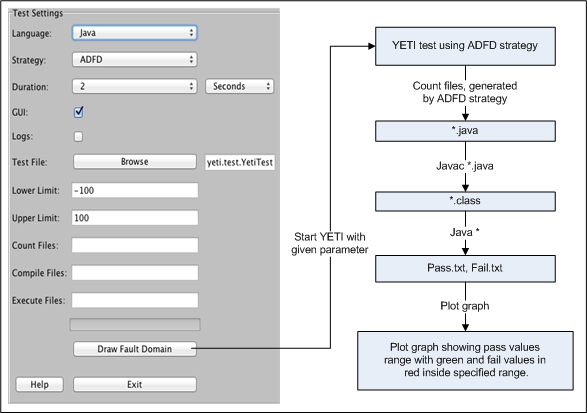
\includegraphics[width=8.2cm,height=6cm]{ADFD/ADFD-Diagram1.png}
\caption{Work flow of ADFD strategy}
\label{fig:ADFD}
\end{figure}

\begin{figure}[htp]
\begin{center}
%\centring
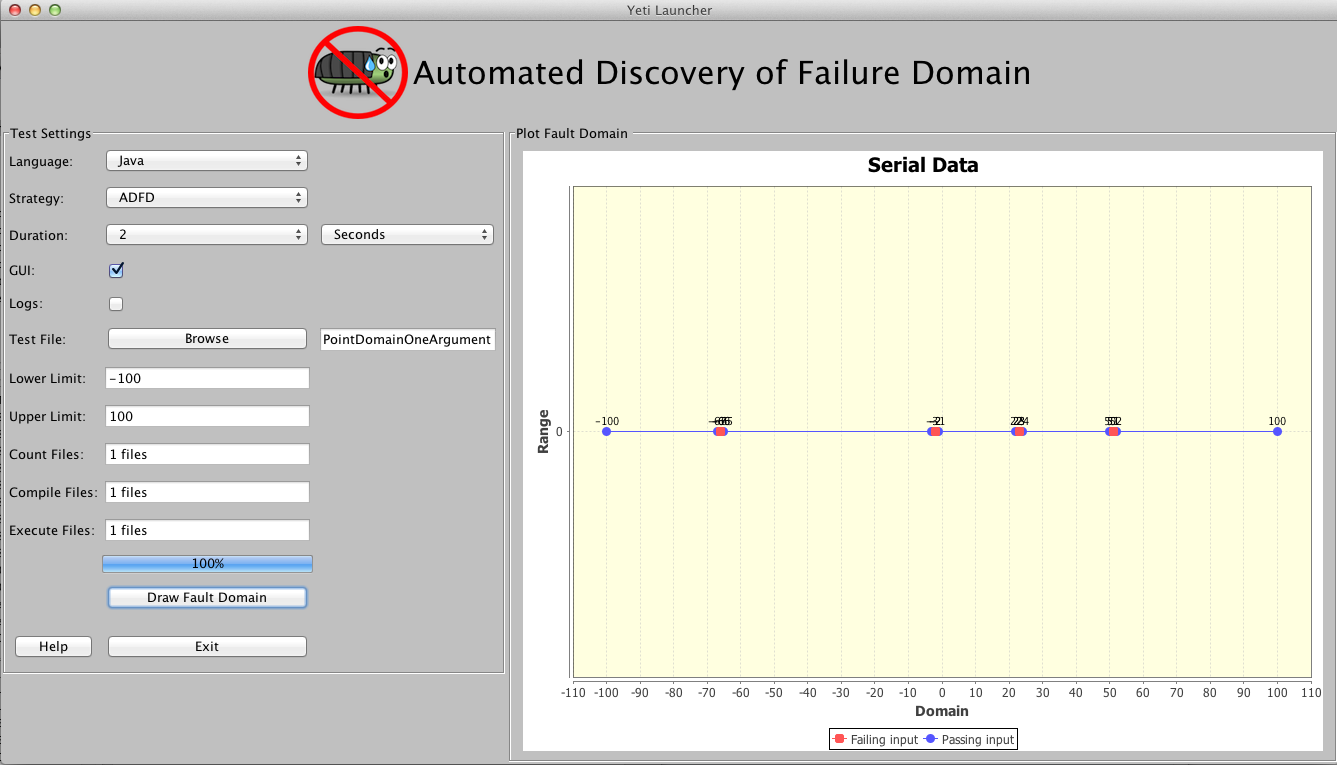
\includegraphics[width=12cm,height=6.6cm]{ADFD/ADFD-front-end.png}
\caption{Front-end of ADFD strategy}
\label{fig:ADFD}
\end{center}
\end{figure}

\noindent \textbf{GUI front-end for providing input:}\\*
\indent ADFD strategy is provided with an easy to use GUI front-end to get input from the user. It takes YETI specific input including language of the program, strategy, duration, enable or disable YETI GUI, logs and a program to test in the form of java byte code. In addition it also takes minimum and maximum values to search for fault domain in the specified range. Default range for minimum and maximum is Integer.MIN\_INT and Integer.MAX\_INT respectively.\\

\noindent \textbf{Automated finding of fault:}\\*
\indent To find the failure domain for a specific fault, the first requirement is to identify that fault in the system. ADFD strategy extends R+ strategy and rely on R+ strategy to find the first fault. Random+ (R+) is an improvement over random strategy with preference to the boundary values to provide better fault finding ability. ADFD strategy is implemented in YETI tool which is famous for its simplicity, high speed and proven ability of finding potentially hazardous faults in many systems \cite{Oriol2011},  \cite{Oriol2012}. YETI is quick and can call up to one million instructions in one second on Java code. It is also capable of testing VB.Net, C, JML and CoFoJa beside Java. \\

\noindent \textbf{Automated generation of modules:}\\*
\indent  After a fault is found in the SUT, ADFD strategy generate complete new Java program to search for fault domains in the given SUT.  These programs with ``.java" extensions are generated through dynamic compiler API included in Java 6 under javax.tools package. The number of programs generated can be one or more, depending on the number of arguments in the test module i.e. for module with one argument one program is generated, for two argument two programs and so on. To track fault domain the program keeps one or more than one argument constant and only one argument variable in the generated program.\\

\noindent \textbf{Automated compilation and execution of modules to discover domains:}\\*
\indent  The java modules generated in previous step are compiled using ``javac *" command to get their binary ``.class" files. The ``java *" command is applied to execute the compiled programs. During execution the constant arguments of the module remain the same but the variable argument receive all the values in range, from minimum to maximum, specified in the beginning of the test. After execution is completed we get two text files of ``Pass.txt" and ``Fail.txt". Pass file contains all the values for which the modules behave correctly while fail file contains all the values for which the modules fail.\\

\noindent \textbf{Automated generation of graph showing domains:}\\*
\indent The values from the pass and fail files are used to plot (x, y) chart using JFreeChart. JFreeChart is a free open-source java library that helps developers to display complex charts and graphs in their applications \cite{Gilbert2008}. Green colour lines with circle represents pass values while red colour line with squares represents the fail values. Resultant graph clearly depicts both the pass and fail domain across the specified input domain. The graph shows red points in case the program fails for only one value, blocks when the program fails for multiple values and strips when a program fails for a long range of values.%\subsection{Flow Chart of the process}

%The following flow chart clearly identify the workflow of the whole process and the various steps involved in the process.

%\begin{figure}[p]
%\centering
%\includegraphics[width=8cm,height=12cm]{automatedFail.png}
%\caption{Automated discovery of Failure Domain}
%\label{fig:autofail}
%\end{figure}




%We found that it is better for the developer to see the range because the fault can be found once but it can generate errors at multiple locations.like point pattern in the first graph only generate fault at location 0 but if the same zero is assigned to second argument then the whole domain values can fail.\\


%\begin{figure}[htp]
%\centering
%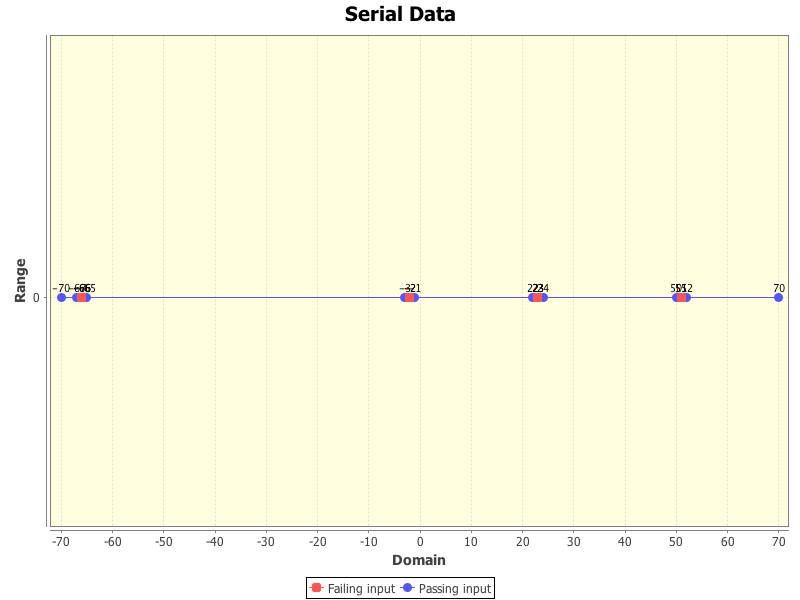
\includegraphics[width=8.5cm,height=6cm]{oneArgumentPointDomain.png}
%\caption{Point pattern failure domain}
%\label{fig:patterns}
%\end{figure}


%Figure \ref{fig:point} shows the example of point pattern. In sub figure \ref{fig1:a} test only fails for 0 out of the whole integer range where as in sub figure \ref{fig1:b} all test fails when static variable is assigned with 0 value.


%\begin{figure}[htp]
%\centering
%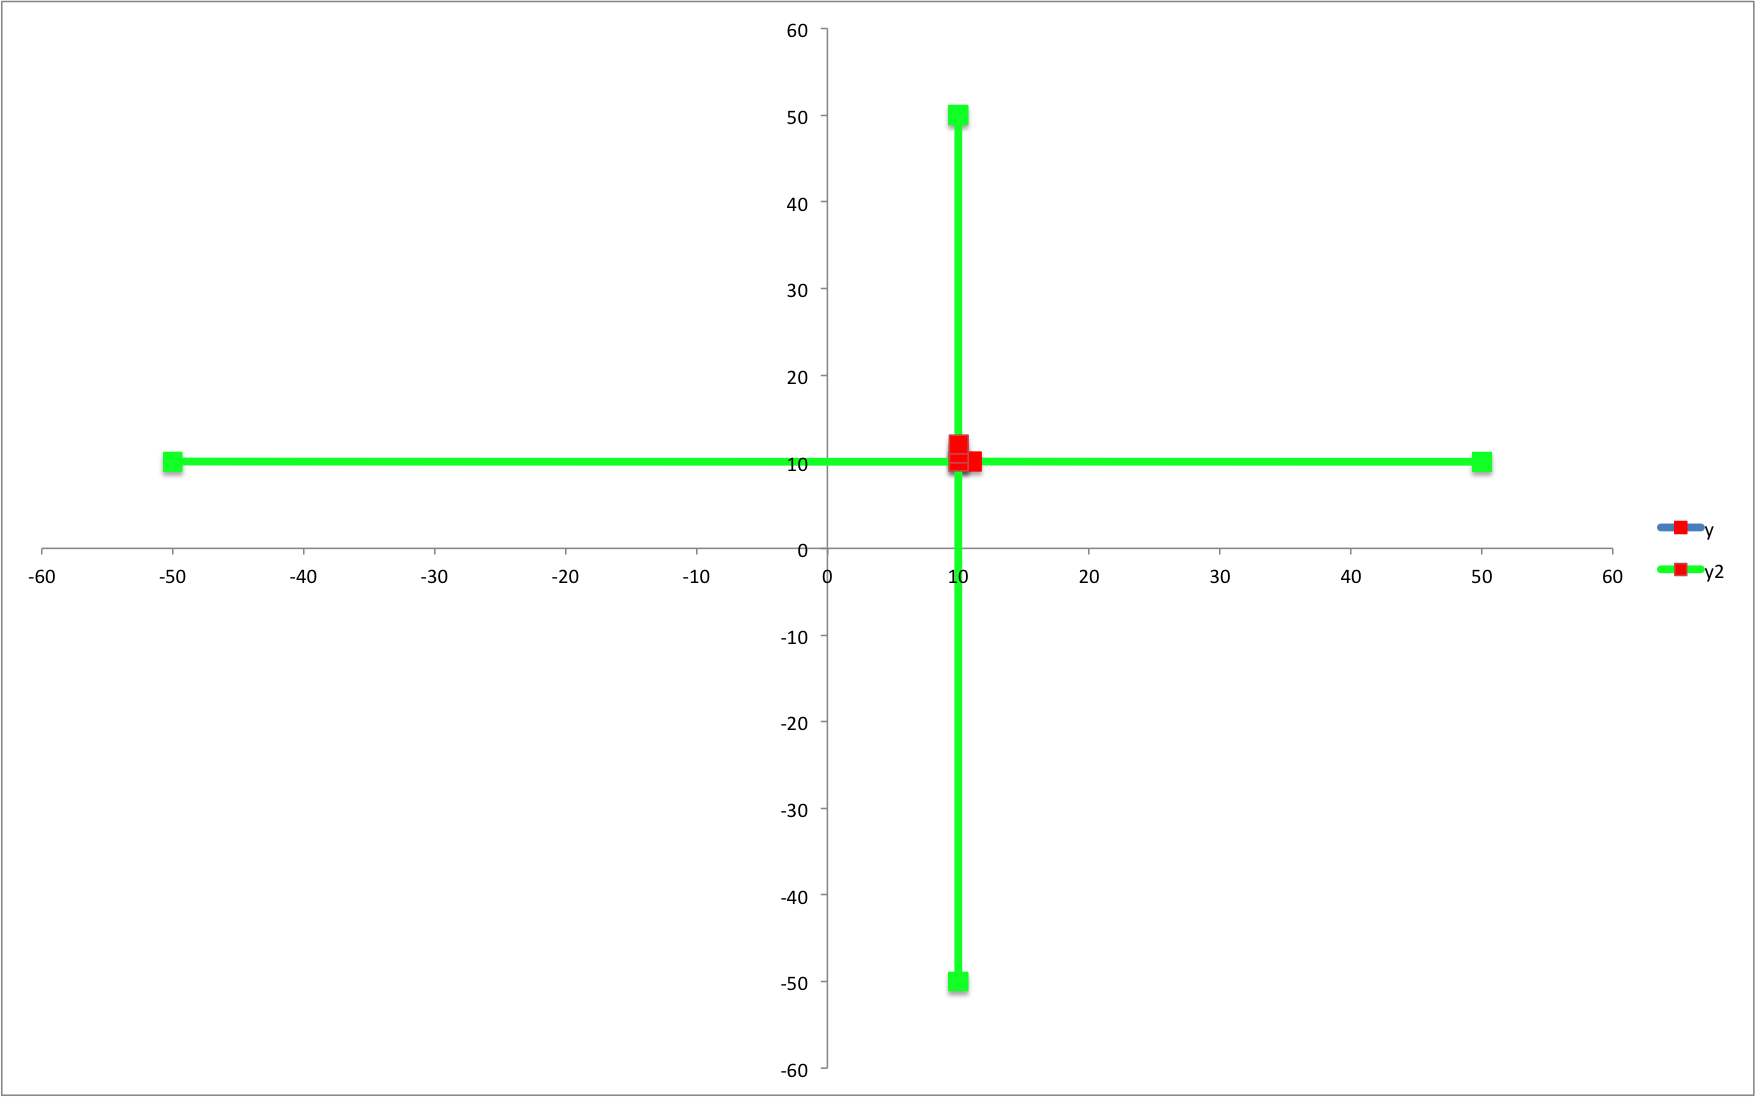
\includegraphics[width=4cm,height=4cm]{block_pattern.png}
%\caption{Block pattern failure domain}
%\label{fig:patterns}
%\end{figure}


%Figure \ref{fig:block} shows the example of block pattern. Both sub figure \ref{fig1:a} and \ref{fig1:b} shows the block pattern of failure. The failure values are given in table \ref{tb:failtable}.

%\begin{figure}[htp]
%\centering
%\begin{center}
%  % Maximum length
 %\subfloat[Test 1 A]{\label{fig1:a}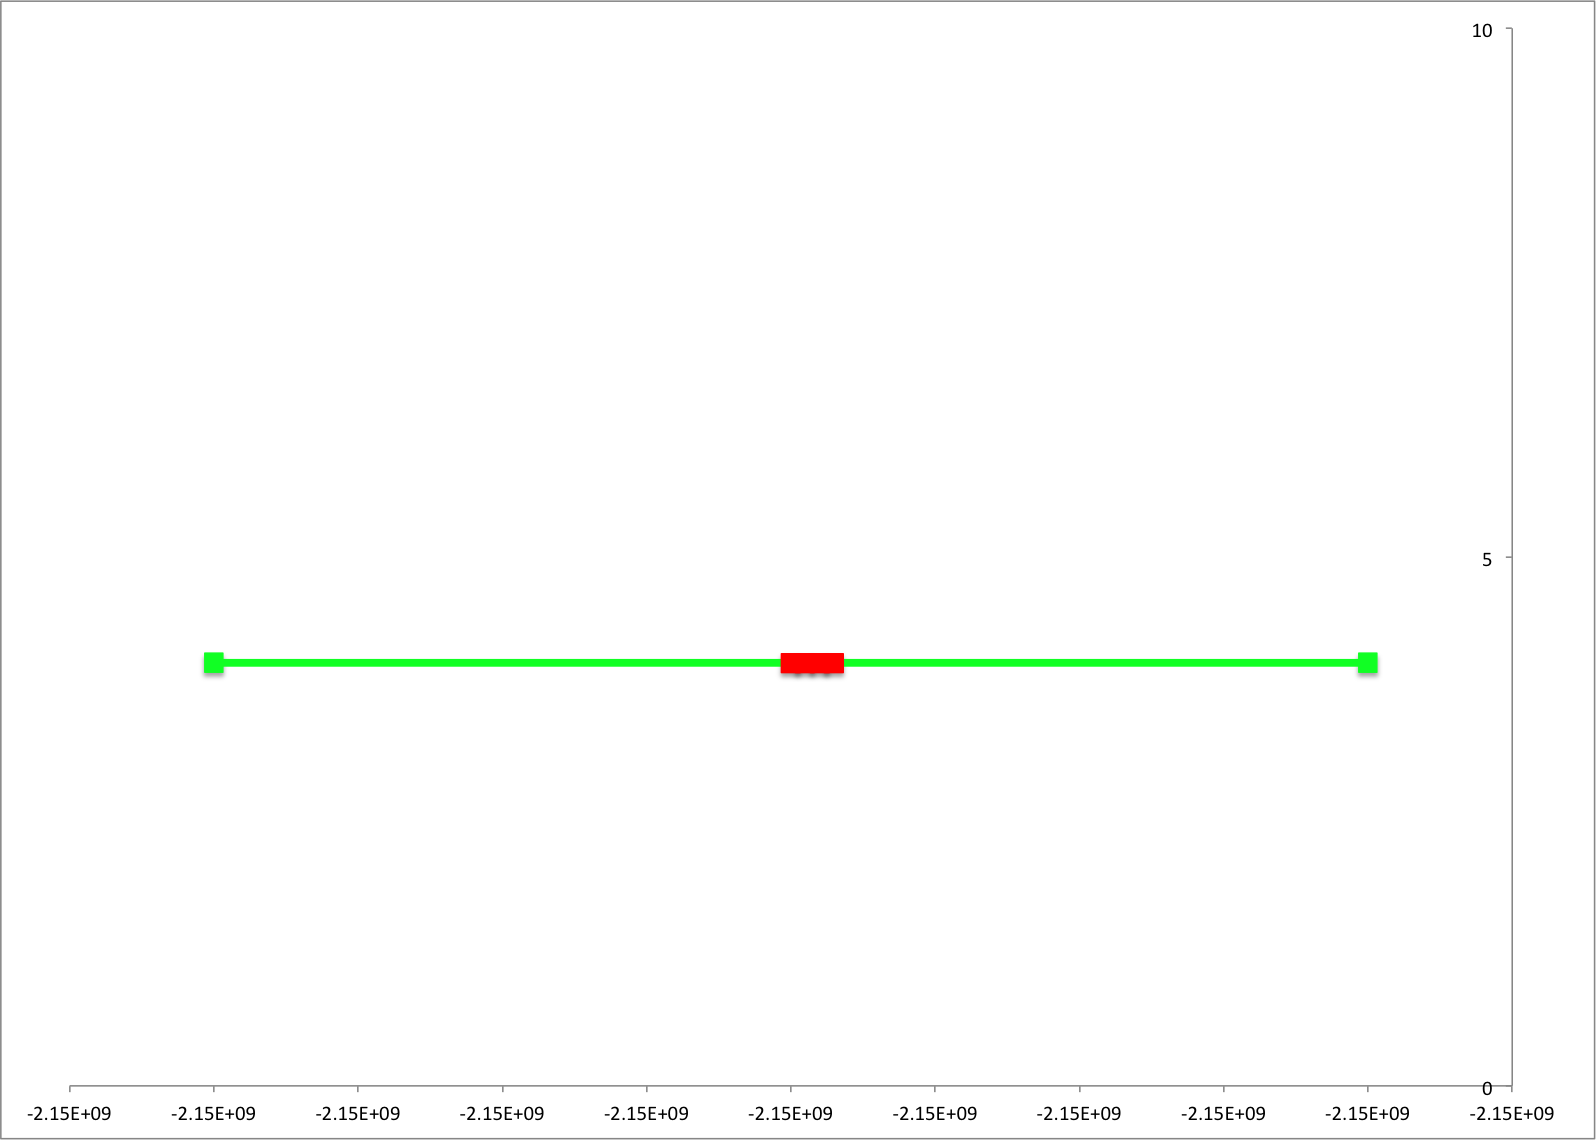
\includegraphics[width=0.49\linewidth]{excel_png/strip_pattern_B.png}}\hfill
 %\subfloat[Test 1 B]{\label{fig1:b}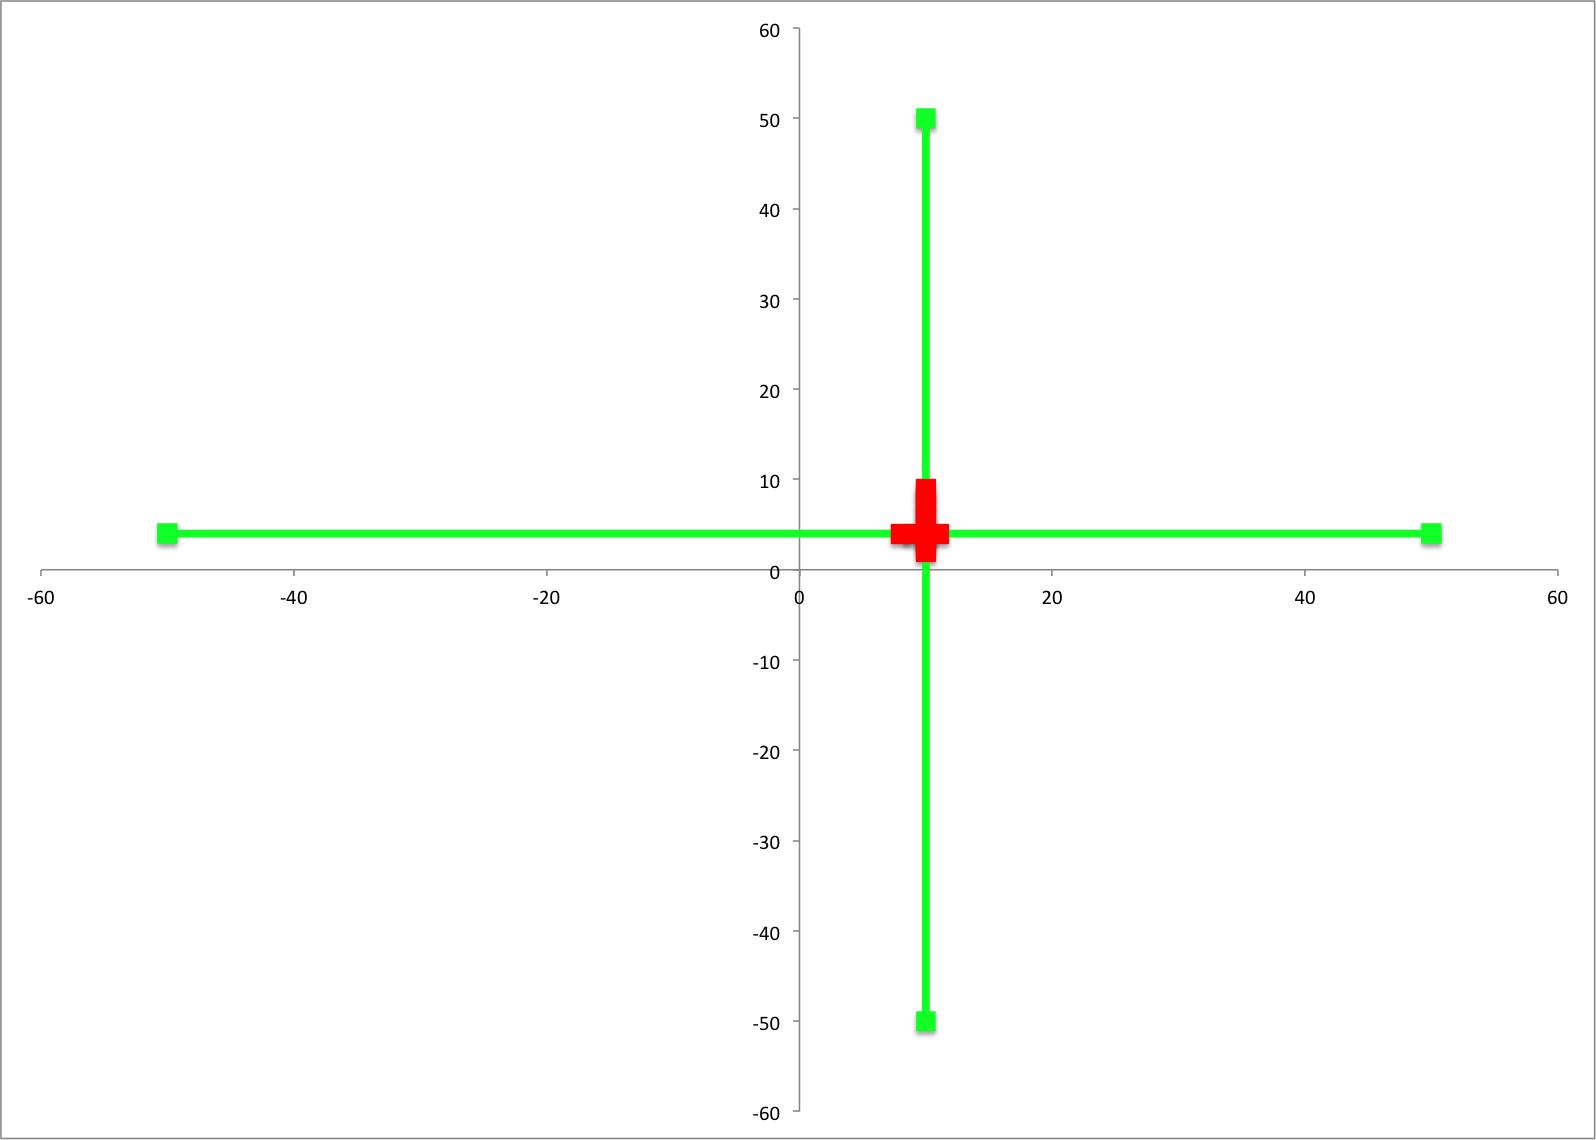
\includegraphics[width=0.49\linewidth]{excel_png/strip_pattern_A.png}}
%  end{center}
%\caption{Strip pattern failure domain}
%%  \label{fig:strip}
%\end{figure}

%Figure shows the example of strip pattern. Here we have two strip failure pattern for test 1 shown in \ref{fig1:a} and \ref{fig1:b} while 1 other for test 2 given in . The failure values are given in table .\\

\section{Implementation}\label{sec:implementation}
The ADFD strategy is implemented in a tool called York Extensible Testing Infrastructure (YETI). YETI is available in open-source at \url{http://code.google.com/p/yeti-test/}. In this section a brief overview of YETI is given with the focus on the parts relevant to the implementation of ADFD strategy. For integration of ADFD strategy in YETI, a program is used as an example to illustrate the working of ADFD strategy. Please refer to  \cite{Oriol2011},  \cite{Oriol2012}, \cite{Oriol2010}, \cite{Oriol2010b} for more details on YETI tool.

 \subsection{York Extensible Testing Infrastructure}
YETI is a testing tool developed in Java that test programs using random strategies in an automated fashion. YETI meta-model is language-agnostic which enables it to test programs written in functional, procedural and object-oriented languages.

YETI consists of three main parts including core infrastructure for extendibility through specialisation, strategies section for adjustment of multiple strategies and languages section for supporting multiple languages. Both the languages and strategies sections have a pluggable architecture to easily incorporate new strategies and languages making YETI a favourable choice to implement ADFD strategy. YETI is also capable of generating test cases to reproduce the faults found during the test session.
 
 \subsection{ADFD strategy in YETI}
The strategies section in YETI contains all the strategies including random, random+ and DSSR to be selected for testing according to the specific needs. The default test strategy for testing is random. On top of the hierarchy in strategies, is an abstract class YetiStrategy, which is extended by YetiRandomPlusStrategy and it is further extended to get ADFD strategy.
% as shown in figure \ref{fig:hierarchy}. 
 
%\begin{figure}[h]
%\centering
%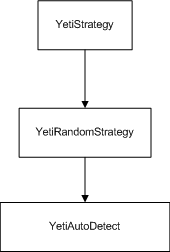
\includegraphics[width=3cm,height=3.5cm]{Hierarchy1.png}
%\caption{Class Hierarchy of automated discovery of failure domains in YETI}
%\label{fig:hierarchy}
%\end{figure}

\subsection{Example}\label{sec:example}
For a concrete example to show how ADFD strategy in YETI proceeds, we suppose YETI tests the following class with ADFD strategy selected for testing. Note that for more clear visibility of the output graph generated by ADFD strategy at the end of test session, we fix the values of lower and upper range by 70 from Integer.MIN\_INT and Integer.MAX\_INT. 

\begin{lstlisting}
/**
 * Point Fault Domain example for one argument
 * @author (Mian and Manuel)
 */
public class PointDomainOneArgument{
	public static void pointErrors (int x){
     		if (x == -66)
       			abort();
     
     		if (x == -2)
     			abort();
      				
     		if (x == 51)
     			abort();
     
     		if (x == 23)
     			abort();
	}
}
\end{lstlisting}

%Published programs from literature \cite{Chen2003}\cite{Chan1996}\cite{Chen2004} of point, block and strip failure patterns are tested to explain the working of ADFD . These programs were translated in to java language for this experiment (See appendix 1 for more details). 

\begin{figure}[H]
\centering
\includegraphics[width=8.2cm,height=3.5cm]{ADFD/pointDomainOneArgument.png}
\caption{ADFD strategy plotting pass and fault domain of the given class}
\label{fig:ADFD-example}
\end{figure}

As soon as any one of the above four faults are discovered the ADFD strategy generate a dynamic program given in Appendix \ref{sec:appendix1} (1). This program is automatically compiled to get binary file and then executed to find the pass and fail domains inside the specified range. The identified domains are plotted on two-dimensional graph. It is evident from the output presented in Figure \ref{fig:ADFD-example} that ADFD strategy not only finds all the faults but also the pass and fail domains.


\begin{comment}
%%%%%% They are commented in this format to decrease the text, for two column format uncomment them.

ADFD can be activated by typing the command java -jar ADFD.jar. After the GUI of ADFD is launched we need to specify yeti specific values that include language of the program under test, strategy for the current test session, duration of test session (minutes or milli-second), display YETI GUI or not and display real time logs or not. Next we browse to select the file for testing and the run button starts testing the file with YETI tool. 

\begin{figure}[ht]
\centering
\includegraphics[width=8.2cm,height=5cm]{pointDomainOneArgument.png}
\caption{ADFD strategy plotting pass and fault domain of the given class}
\label{fig:ADFD-example}
\end{figure}

In 5 second YETI found one fault out of the above 4 faults. The ADFD strategy in YETI generate a source file (C*.java) at the end of the test session. This file contain the code that searches for fault domains. The count button count the number of files. ADFD create the number of files on the basis of the number of arguments in the method under test. For one argument one method is created and for two argument two methods are created. 

The next button is compile which compile the generated files and generate the byte code (.class files). The execute button execute the byte code and test the method under test for all the values between upper and lower bound. At the end of execution it generates two files (pass.txt and fail.txt). Pass file contain all the values for which the method performed correctly while fail file contain all the values for which the method under test fail.

The draw fault domain button reads the pass and fail files and plot them on the x, y graph where red line with squares show the failing values while the blue line with square shapes show the passing values.
\end{comment}

%%%%%%%%%%%%%%%%%%%%%%%%%%%%%%%%%%%%%%%%%%%%%%%%%%%%%%%%

\section{Experimental Results} \label{sec:experimentalResults}
This section includes the experimental setup and results obtained after using ADFD strategy. Six numerical programs of one and two-dimension were selected. These programs were error-seeded in such a way to get all the three forms of fault domains including point, block and strip fault domains. Each selected program contained various combinations of one or more fault domains. 

All experiments were performed on a 64-bit Mac OS X Lion Version 10.7.5 running on 2 x 2.66 GHz 6-Core Intel Xeon with 6.00 GB (1333 MHz DDR3) of RAM. YETI runs on top of the Java\texttrademark  SE Runtime Environment [version 1.6.0\_35]. 

To elucidate the results, six programs were developed so as to have separate program for one and two-dimension point, block and strip fault domains. The code of selected programs is given in Appendix \ref{sec:appendix1} (2-7). The experimental results are presented in table \ref{sec:fail table} and described under the following three headings.
%\begin{center}

%\end{center}

\begin{table}[h]
%\renewcommand{\arraystretch}{2}
\centering
\scriptsize
%\normalsize

\begin{tabular}{|c|c|c|l|l|l|}

\hline 


\multirow{2}{*}{S. No}	& \multirow{2}{*}{Fault }	 				& \multirow{2}{*}{Module } 		& \multirow{2}{*}{Specific Fault}	 		& \multirow{2}{*}{Pass Domain} 					& \multirow{2}{*}{Fail Domain} 			\\  
					& Domain								&  Dimension					&									&											&								\\ \hline 
\multirow{6}{*}{1} 	&	\multirow{6}{*}{Point}				& 	\multirow{3}{*}{One}			&	\multirow{3}{*}{PFDOneA(i)}	&	-100 to -67, -65 to -3, 		  		& -66, -2, 23, 51			 	\\  
				&									&							&							&	-1 to 50, 2 to 22, 					&							\\  
				&									&							&							&	24 to 50, 52 to 100					&							\\ \cline{3-6}
				&									&	\multirow{3}{*}{Two}			&	\multirow{2}{*}{PFDTwoA(2, i)}	&	(2, 100) to (2, 1),	 				&  (2, 0)						\\  
				&									&							&							&	(2, -1) to (2, -100)					&							\\ \cline{4-6}
				&									& 							&	PFDTwoA(i, 0)				&	Nil								& (-100, 0) to (100, 0)				\\  \hline



\multirow{5}{*}{2} 	&	\multirow{5}{*}{Block}				& 	\multirow{2}{*}{One}			&	\multirow{2}{*}{BFDOneA(i)}	&	-100 to -30, -25 to -2, 					& 	-1 to 1, -29 to -24,		 	\\ 
				&									&							&							&	2 to 50, 55 to 100						&	51 to 54,				\\   \cline{3-6}
				&									&	\multirow{3}{*}{Two}			&	\multirow{2}{*}{BFDTwoA(-2, i)}	&	(-2, 100) to (-2, 20), 					& 	(-2 , 1) to ( -2, 19), 		\\ 
				&									&							&							&      (-2, -1) to (-2, -100)					&	(-2, 0)				\\ \cline{4-6}
				&									& 							&	BFDTwoA(i, 0)				&	Nil								& 	(-100, 0) to (100, 0)		\\  \hline
				
				



\multirow{5}{*}{3} 	&	\multirow{5}{*}{Strip}					& 	\multirow{2}{*}{One}			&	\multirow{2}{*}{SFDOneA(i)}	&	\multirow{2}{*}{-100 to -5, 35 to 100}		& 	\multirow{2}{*}{-4, 34	}\\ 
				&									&							&							&									&				\\  \cline{3-6}
				&									&	\multirow{3}{*}{Two}			&	\multirow{2}{*}{SFDTwoA(-5, i)}	&	(-5, 100) to (-5, 40),					&  (-5, 39) to (-5, 1), 			\\ 
				&									&							&							&	 (-5, 0) to (-5, -100)					&	(-5, 0)				\\ \cline{4-6}
				&									& 							&	SFDTwoA(i, 0)				&	Nil								&  (-100, 0) to (100, 0)			\\  \hline
				
				
\end{tabular}
\bigskip
\caption{Pass and Fail domain with respect to one and two dimensional program}
\label{tab:failtable}
\end{table}




\noindent \textbf{Point Fault Domain:}  Two separate Java programs Pro2 and Pro3 given in Appendix \ref{sec:appendix1} (2, 3) were tested with ADFD strategy in YETI to get the findings for point fault domain in one and two-dimension program. Figure \ref{fig:PFDOne} present range of pass and fail values for point fault domain in one-dimension whereas Figure \ref{fig:PFDTwo} present range of pass and fail values for point fault domain in two-dimension program. The range of pass and fail values for each program in point fault domain are given in (Table \ref{tab:failtable}, Serial No. 1).
%%%%%%%%%%%%%%%%Point Domain%%%%%%%%%%%%%%%%%%%%%%%%%%%%%

\begin{figure} [H]

\subfigure[One dimension module]{
\includegraphics[width=6cm,height=4cm]{ADFD/PFDOne.png}
\label{fig:PFDOne}
}
\subfigure[Two dimension module]{
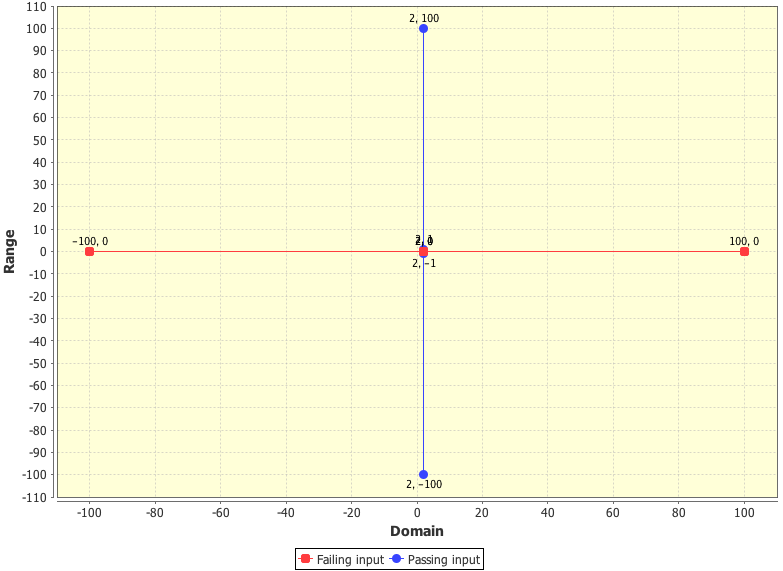
\includegraphics[width=6cm,height=4cm]{ADFD/PFDTwo.png}
\label{fig:PFDTwo}
}


\caption{Chart generated by ADFD strategy presenting point fault domain}
\end{figure}

%\begin{figure}[H]
%\centering
%\includegraphics[width=8.2cm,height=5cm]{PFDOne.png}
%\caption{Chart generated by ADFD strategy presenting point fault domain in one dimension module}
%\label{fig:PFDOne}
%\end{figure}

%\begin{figure}[H]
%\centering
%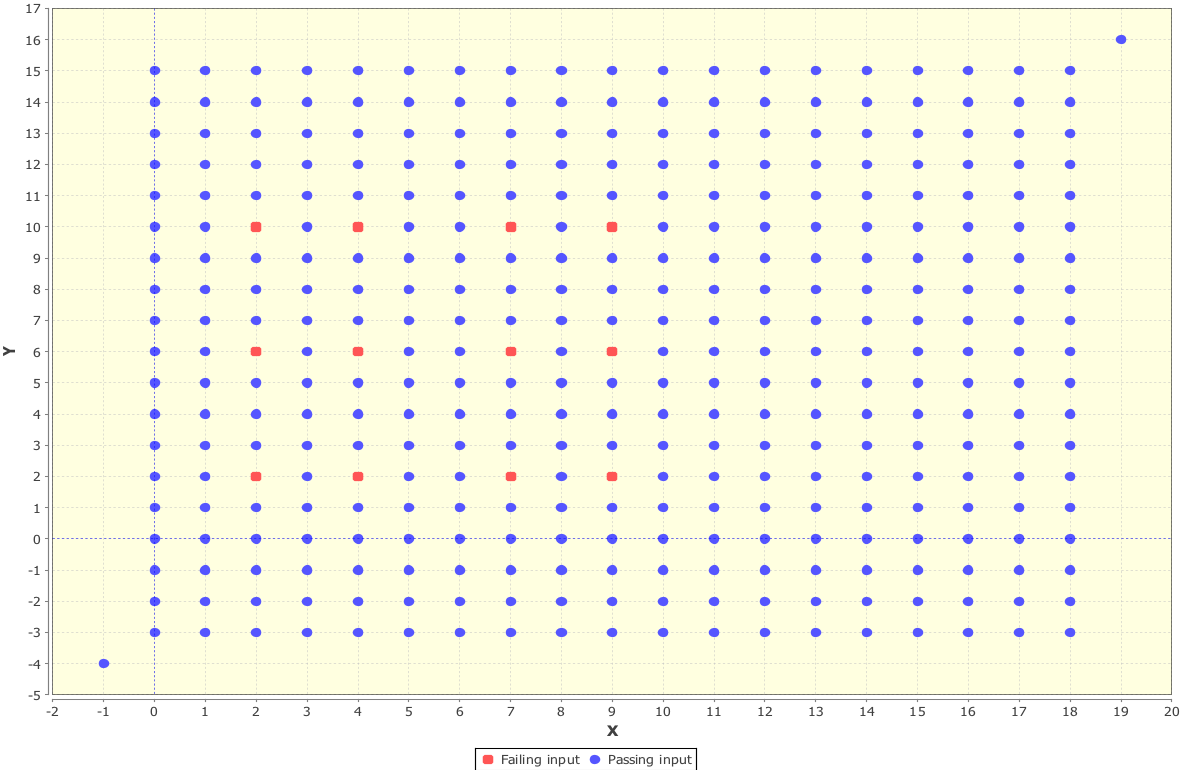
\includegraphics[width=8.2cm,height=5cm]{PFDTwo.png}
%\caption{Chart generated by ADFD strategy presenting point fault domain in two dimension module}
%\label{fig:PFDTwo}
%\end{figure}


\noindent \textbf{Block Fault Domain:}  Two separate Java programs Pro4 and Pro5 given in Appendix \ref{sec:appendix1} (4, 5) were tested with ADFD strategy in YETI to get the findings for block fault domain in one and two-dimension program. Figure \ref{fig:BFDOne} present range of pass and fail values for block fault domain in one-dimension whereas Figure \ref{fig:BFDTwo} present range of pass and fail values for block fault domain in two-dimension program. The range of pass and fail values for each program in block fault domain are given in (Table \ref{tab:failtable}, Serial No. 2).
%%%%%%%%%%%%%%%Block domain %%%%%%%%%%%%%%%%%%%%%%%%%%%%%%
%%%





\begin{figure} [H]

\subfigure[One dimension module]{
\includegraphics[width=6cm,height=4cm]{ADFD/BFDOne.png}
\label{fig:BFDOne}
}
\subfigure[Two dimension module]{
\includegraphics[width=6cm,height=4cm]{ADFD/BFDTwo.png}
\label{fig:BFDTwo}
}


\caption{Chart generated by ADFD strategy presenting block fault domain}
\end{figure}


%\begin{figure}[H]
%\centering
%\includegraphics[width=8.2cm,height=5cm]{BFDOne.png}
%\caption{Chart generated by ADFD strategy presenting block fault domain in one dimension module}
%\label{fig:BFDOne}
%\end{figure}


%\begin{figure}[H]
%\centering
%\includegraphics[width=8.2cm,height=5cm]{BFDTwo.png}
%\caption{Chart generated by ADFD strategy presenting block fault domain in two dimension module}
%\label{fig:BFDTwo}
%\end{figure}



\noindent \textbf{Strip Fault Domain:} Two separate Java programs Pro6 and Pro7 given in Appendix \ref{sec:appendix1} (6, 7) were tested with ADFD strategy in YETI to get the findings for strip fault domain in one and two-dimension program. Figure \ref{fig:SFDOne} present range of pass and fail values for strip fault domain in one-dimension whereas Figure \ref{fig:SFDTwo} present range of pass and fail values for strip fault domain in two-dimension program. The range of pass and fail values for each program in strip fault domain are given in (Table \ref{tab:failtable}, Serial No. 3).


%
%%%%%%%%%%%%%%%%%%%%%%Strip domain %%%%%%%%%%%%%%%%%%%%%%%
\begin{figure} [H]

\subfigure[One dimension module]{
\includegraphics[width=6cm,height=4cm]{ADFD/SFDOne.png}
\label{fig:SFDOne}
}
\subfigure[Two dimension module]{
\includegraphics[width=6cm,height=4cm]{ADFD/SFDTwo.png}
\label{fig:SFDTwo}
}


\caption{Chart generated by ADFD strategy presenting Strip fault domain}
\end{figure}






%\begin{figure}[H]
%\centering
%\includegraphics[width=8.2cm,height=5cm]{SFDOne.png}
%\caption{Chart generated by ADFD strategy presenting strip fault domain in one dimension module}
%\label{fig:SFDOne}
%\end{figure}

%\begin{figure}[H]
%\centering
%\includegraphics[width=8.2cm,height=5cm]{SFDTwo.png}
%\caption{Chart generated by ADFD strategy presenting strip fault domain in two dimension module}
%\label{fig:SFDTwo}
%\end{figure}



\section{Discussion} \label{sec:discussion}

ADFD strategy with a simple graphical user interface is a fully automated process to identify and plot the pass and fault domains on the chart. Since the default settings are all set to optimum the user needs only to specify the module to be tested and click ``Draw fault domain" button to start test execution. All the steps including Identification of fault, generation of dynamic java program to find domain of the identified fault, saving the program to a permanent media, compiling the program to get its binary, execution of binaries to get pass and fail domain and plotting these values on the graph are done completely automated without any human intervention.

In the experiments (section \ref{sec:experimentalResults}), the ADFD strategy effectively identified faults and faults domain in a program. Identification of fault domain is simple for one and two dimension numerical program but the difficulty increases as the program dimension increases beyond two. Similarly no clear boundaries are defined for non-numerical data therefore it is not possible to plot domains for non-numerical data unless some boundary criteria is defined.

ADFD strategy initiate testing with random+ strategy to find the fault and later switch to brute-force strategy to apply all the values between upper and lower bound for finding pass and fault domain. 
It is found that faults at boundary of the input domain can pass unnoticed through ordinary random test strategy but not from ADFD strategy as it scan all the values between lower and upper range.


The overhead in terms of execution time associated with ADFD strategy is dependent mainly on the lower and upper bound. If the lower and upper bound is set to maximum range (i.e. minimum for int is Integer.MIN\_INT and maximum Integer.MAX\_INT) then the test duration is maximum. It is rightly so because for identification of fault domain the program is executed for every input available in the specified range. Similarly increasing the range also shrinks the produced graph making it difficult to identify clearly point, block and strip domain unless they are of considerable size. Beside range factor, test duration is also influenced by the identification of the fault and the complexity of module under test.

ADFD strategy can help the debuggers in two ways. First, it reduces the to and from movement of the project between the testers and debuggers as it identity all the faults in one go. Second, it identifies locations of all fault domains across the input domain in a user-friendly way helping debugger to fix the fault keeping in view its all occurrences.


\section{Threats to Validity} \label{sec:validity}
The major external threat to the use of ADFD strategy on commercial scale is the selection of small set of error-seeded programs of only primitive types such as integer used in the experiments. However, the present study will serve as foundation for future work to expand it to general-purpose real world production application containing scalar and non-scalar data types.

Another issue is the easy plotting of numerical data in the form of distinctive units, because it is difficult to split the composite objects containing many fields into units for plotting. Some work has been done to quantify composite objects into units on the basis of multiple features\cite{Ciupa2006},to facilitate easy plotting. Plotting composite objects is beyond the scope of the present study. However, further studies are required to look in to the matter in depth. 

Another threat to validity includes evaluating program with complex and more than two input arguments. ADFD strategy has so far only considered scalar data of one and two-dimensions. However, plotting domain of programs with complex non-scalar and more than two dimension argument is much more complicated and needs to be taken up in future studies.

Finally, plotting the range of pass or fail values for a large input domain (Integer.MIN\_INT to Integer.MAX\_INT) is difficult to adjust and does not give a clearly understandable view on the chart. Therefore zoom feature is added to the strategy to zoom into the areas of interest on the chart.



\section{Related Works} \label{sec:relatedWork}
Traditional random testing is quick, easy to implement and free from any bias. In spite of these benefits, the lower fault finding ability of traditional random testing is often criticised \cite{Offutt1996}, \cite{Myers2011}. To overcome the performance issues without compromising on its benefits, various researchers have altered its algorithm as explained in section 1. Most of the alterations are based on the existence of faults and fault domains across the input domain \cite{Chan1996}. 

Identification, classification of pass and fail domains and visualisation of domains have not received due attention of the researchers. Podgurski et. al., \cite{Podgurski2003} proposed a semi-automated procedure to classify similar faults and plot them by using a Hierarchical Multi Dimension Scaling (HMDS) algorithm. A tool named Xslice \cite{Agrawal1995} visually differentiates the execution slices of passing and failing part of a test. Another tool called Tarantula uses colour coding to track the statements of a program during and after the execution of the test suite \cite{Jones2002}. A serious limitation of the above mentioned tools is that they are not fully automated and require human interaction during execution. Moreover these tools are based on the already existing test cases where as ADFD strategy generate test cases, discover faults, identify pass and fault domains and visualise them in a fully automated manner. 


\section{Conclusion} \label{sec:conclusion}

Results of the experiments (section 4), based on applying ADFD strategy to error-seeded numerical programs provide, evidence that the strategy is highly effective in identifying the faults and plotting pass and fail domains of a given SUT. It further suggests that the strategy may prove effective for large programs. However, it must be confirmed with programs of more than two-dimension and different non-scalar argument types. ADFD strategy can find boundary faults quickly as against the traditional random testing, which is either, unable or takes comparatively long time to discover the faults.

The use of ADFD strategy is highly effective in testing and debugging. It provides an easy to understand test report visualising pass and fail domains. It reduces the number of switches of SUT between testers and debuggers because all the faults are identified after a single execution. It improves debugging efficiency as the debuggers keep all the instances of a fault under consideration when debugging the fault.






% ------------------------------------------------------------------------


%%% Local Variables: 
%%% mode: latex
%%% TeX-master: "../thesis"
%%% End: 

%\chapter{Sample Title}

Lorem ipsum dolor sit amet, consectetur adipiscing elit, sed do eiusmod tempor incididunt ut labore et dolore magna aliqua. Ut enim ad minim veniam, quis nostrud exercitation ullamco laboris nisi ut aliquip ex ea commodo consequat. Duis aute irure dolor in reprehenderit in voluptate velit esse cillum dolore eu fugiat nulla pariatur. Excepteur sint occaecat cupidatat non proident, sunt in culpa qui officia deserunt mollit anim id est laborum.

\backmatter % book mode only
\appendix
\chapter{  }
\label{chap:appendix1}
\section{Sample code to identify failure domains}
\label{sec:appendix1}
\scriptsize

\section{Error-seeded code to evaluate the performance of ADFD and ADFD+}
%%%%%%%%%%%%%%%%%%%%%%%%%%%%%%%%%%%%%%%%%%%%%%%%%%%%%%%%%%%%%%%%%%%%%%%%%%%%%%%%%%%%%%%%%%%%%%
\textbf{Program 1} Point domain with One argument
\begin{lstlisting} 
/**
 * Point Fault Domain example for one argument
 * @author (Mian and Manuel)
 */
public class PointDomainOneArgument{

	public static void pointErrors (int x){
		if (x == -66 )
			x = 5/0;

		if (x == -2 )
			x = 5/0;

		if (x == 51 )
			x = 5/0;

		if (x == 23 )
			x = 5/0;
	}
}
\end{lstlisting}
%%%%%%%%%%%%%%%%%%%%%%%%%%%%%%%%%%%%%%%%%%%%%%%%%%%%%%%%%%%%%%%%%%%%%%%%%%%%%%%%%%%%%%%%%%%%%%
\textbf{Program 2} Point domain with two argument
\begin{lstlisting}
/**
 * Point Fault Domain example for two arguments
 * @author (Mian and Manuel)
 */
public class PointDomainOneArgument{

	public static void pointErrors (int x, int y){
		int z = x/y;
	}

}
\end{lstlisting}

%%%%%%%%%%%%%%%%%%%%%%%%%%%%%%%%%%%%%%%%%%%%%%%%%%%%%%%%%%%%%%%%%%%%%%%%%%%%%%%%%%%%%%%%%%%%%%
\textbf{Program 3} Block domain with one argument
\begin{lstlisting}
/**
 * Block Fault Domain example for one arguments
 * @author (Mian and Manuel)
 */

public class BlockDomainOneArgument{

public static void blockErrors (int x){
	
	if((x > -2) \&\& (x < 2))
		x = 5/0;
	
	if((x > -30) \&\& (x < -25))
		x = 5/0;
	
	if((x > 50) \&\& (x < 55))
		x = 5/0;

   }
}

\end{lstlisting}
%%%%%%%%%%%%%%%%%%%%%%%%%%%%%%%%%%%%%%%%%%%%%%%%%%%%%%%%%%%%%%%%%%%%%%%%%%%%%%%%%%%%%%%%%%%%%%
\textbf{Program 4} Block domain with two argument
\begin{lstlisting}
/**
 * Block Fault Domain example for two arguments
 * @author (Mian and Manuel)
 */
public class BlockDomainTwoArgument{

	public static void pointErrors (int x, int y){

		if(((x > 0)&&(x < 20)) || ((y > 0) && (y < 20))){
		x = 5/0;
		}
  	
	}

}
\end{lstlisting}
%%%%%%%%%%%%%%%%%%%%%%%%%%%%%%%%%%%%%%%%%%%%%%%%%%%%%%%%%%%%%%%%%%%%%%%%%%%%%%%%%%%%%%%%%%%%%%

\textbf{Program 5} Strip domain with One argument
\begin{lstlisting}
/**
 * Strip Fault Domain example for one argument
 * @author (Mian and Manuel)
 */

public class StripDomainOneArgument{

	public static void stripErrors (int x){
	
		if((x > -5) && (x < 35))
			x = 5/0;
  	 }
}
\end{lstlisting}
%%%%%%%%%%%%%%%%%%%%%%%%%%%%%%%%%%%%%%%%%%%%%%%%%%%%%%%%%%%%%%%%%%%%%%%%%%%%%%%%%%%%%%%%%%%%%%
\textbf{Program 6} Strip domain with two argument
\begin{lstlisting}
/**
 * Strip Fault Domain example for two arguments
 * @author (Mian and Manuel)
 */
public class StripDomainTwoArgument{

	public static void pointErrors (int x, int y){

		if(((x > 0)&&(x < 40)) || ((y > 0) && (y < 40))){
		x = 5/0;
		}
  	
	}

}

\end{lstlisting}
%%%%%%%%%%%%%%%%%%%%%%%%%%%%%%%%%%%%%%%%%%%%%%%%%%%%%%%%%%%%%%%%%%%%%%%%%%%%%%%%%%%%%%%%%%%%%%

Program generated by ADFD on finding fault in SUT
\begin{lstlisting}
/**
 * Dynamically generated code by ADFD strategy 
 * after a fault is found in the SUT.
 * @author (Mian and Manuel)
 */
import java.io.*;
import java.util.*;

public class C0 
{
	public static ArrayList<Integer> pass = new ArrayList<Integer>();
	public static ArrayList<Integer> fail = new ArrayList<Integer>();
	public static boolean startedByFailing = false;
	public static boolean isCurrentlyFailing = false;
	public static int start = -80; 
	public static int stop = 80;

	public static void main(String []argv){
		checkStartAndStopValue(start);
		for (int i=start+1;i<stop;i++){
			try{
				PointDomainOneArgument.pointErrors(i);
				if (isCurrentlyFailing) 
				{
					fail.add(i-1);
					fail.add(0);
					pass.add(i);
					pass.add(0);
					isCurrentlyFailing=false; 
				} 
			} 
			catch(Throwable t) { 
				if (!isCurrentlyFailing) 
				{
					pass.add(i-1);
					pass.add(0);
					fail.add(i);
					fail.add(0);
					isCurrentlyFailing = true;
				}  
			} 
		} 
		checkStartAndStopValue(stop); 
		printRangeFail(); 
		printRangePass();  
	}

	public static void printRangeFail() { 
		try { 
			File fw = new File("Fail.txt"); 
			if (fw.exists() == false) { 
				fw.createNewFile(); 
			}
			PrintWriter pw = new PrintWriter(new FileWriter (fw, true));   
			for (Integer i1 : fail) { 
				pw.append(i1+"\n"); 
			} 
			pw.close(); 
		} 
		catch(Exception e) { 
			System.err.println(" Error : e.getMessage() "); 
		} 
	} 
	public static void printRangePass() { 
		try { 
			File fw1 = new File("Pass.txt"); 
			if (fw1.exists() == false) { 
				fw1.createNewFile(); 
			}
			PrintWriter pw1 = new PrintWriter(new FileWriter (fw1, true));   
			for (Integer i2 : pass) { 
				pw1.append(i2+"\n");
			} 
			pw1.close(); 
		} 
		catch(Exception e) { 
			System.err.println(" Error : e.getMessage() "); 
		} 
	} 
	public static void checkStartAndStopValue(int i) { 
		try { 
			PointDomainOneArgument.pointErrors(i);
			pass.add(i); 
			pass.add(0);
		} 
		catch (Throwable t) { 
			startedByFailing = true; 
			isCurrentlyFailing = true; 
			fail.add(i); 
			fail.add(0);
		} 
	} 
}

\end{lstlisting}
\chapter{Sample Title}

Lorem ipsum dolor sit amet, consectetur adipiscing elit, sed do eiusmod tempor incididunt ut labore et dolore magna aliqua. Ut enim ad minim veniam, quis nostrud exercitation ullamco laboris nisi ut aliquip ex ea commodo consequat. Duis aute irure dolor in reprehenderit in voluptate velit esse cillum dolore eu fugiat nulla pariatur. Excepteur sint occaecat cupidatat non proident, sunt in culpa qui officia deserunt mollit anim id est laborum.

\bibliographystyle{plain}
%\bibliographystyle{Classes/CUEDbiblio}
%\bibliographystyle{Classes/jmb}
%\bibliographystyle{Classes/jmb} % bibliography style
\renewcommand{\bibname}{References} % changes default name Bibliography to References
\bibliography{References/references} % References file

\end{document}
